\documentclass[11pt,reqno]{amsart}
\usepackage[T1]{fontenc}
\usepackage{lmodern}
\usepackage{amsmath,amssymb,amsthm,mathtools}
\usepackage[kerning=true]{microtype}
\usepackage{enumitem,booktabs,graphicx,xcolor}
\usepackage[margin=1.12in]{geometry}
\usepackage{xurl}
\usepackage[colorlinks=true,linkcolor=blue!55!black,citecolor=blue!55!black,
urlcolor=blue!55!black]{hyperref}
\hypersetup{pdftitle={Subexponential Weighted Counting and Exact Optimisation},pdfauthor={Deep Bhattacharjee}}
\emergencystretch=2em
\numberwithin{equation}{section}
\raggedbottom
\theoremstyle{plain}
\newtheorem{theorem}{Theorem}[section]
\newtheorem{lemma}[theorem]{Lemma}
\newtheorem{proposition}[theorem]{Proposition}
\newtheorem{corollary}[theorem]{Corollary}
\theoremstyle{definition}
\newtheorem{definition}[theorem]{Definition}
\theoremstyle{remark}
\newtheorem{remark}[theorem]{Remark}
\newtheorem{example}[theorem]{Example}
\DeclareMathOperator{\Bin}{Bin}
\DeclareMathOperator{\poly}{poly}
\DeclareMathOperator{\rank}{rank}
\DeclareMathOperator{\diag}{diag}
\DeclareMathOperator{\cut}{cut}
\DeclareMathOperator{\sat}{sat}
\DeclareMathOperator{\SE}{SE}
\DeclareMathOperator{\SNP}{SNP}
\newcommand{\A}{\mathcal{A}}
\newcommand{\F}{\mathcal{F}}
\newcommand{\B}{\mathcal{B}}
\newcommand{\Q}{\mathbb{Q}}
\newcommand{\Z}{\mathbb{Z}}
\newcommand{\N}{\mathbb{N}}
\newcommand{\R}{\mathbb{R}}
\newcommand{\Ftwo}{\mathbb{F}_2}
\newcommand{\e}{\mathbf{e}}
\newcommand{\PP}{\vec{P}}
\newcommand{\rhon}{\rho}
\newcommand{\ip}[2]{\langle #1,#2\rangle}
\newcommand{\oai}{OpenAI}
\newcommand{\releaseline}{, release v1.1.0, archived at \href{https://doi.org/10.5281/zenodo.23695835}{doi:10.5281/zenodo.23695835}}
\newcommand{\archiveline}{, release v1.1.0 (2026). \href{https://doi.org/10.5281/zenodo.23695835}{doi:10.5281/zenodo.23695835}}

\title[Subexponential weighted counting]{Subexponential Weighted Counting and Exact Optimisation}
\author{Deep Bhattacharjee}
\address{Formerly, Electro-Gravitational Space Propulsion Laboratory (EGSPL),
Bhubaneswar, Odisha 751030, India}
\address{Formerly, University of Calcutta (Heramba Chandra College), 23/49 Gariahat Road,
Golpark, Kolkata 700029, West Bengal, India}
\email{d.bhattacharjee@erl-forschung.de}
\email{itsdeep@live.com}
\email{egspl@proton.me}
\urladdr{https://orcid.org/0000-0003-0466-750X}
\subjclass[2020]{Primary 68Q25; Secondary 68Q17, 68W40, 05C31, 05C85, 82B20}
\keywords{exponential time hypothesis, weighted counting, independence polynomial, vertex cover}
\date{27 October 2026}

\begin{document}

\begin{abstract}
\emph{The deterministic algorithm of \oai{} that counts the satisfying assignments of a
$k$-CNF in time $2^{o(n)}$ is reproduced in full and extended from counting to
sums of local weights with values in any commutative $\Q$-algebra. The extension gives
deterministic $2^{o(n)}$ algorithms for exact Max-Cut and Max-$k$-SAT on sparse instances,
for the independence polynomial and the maximum independent set of every graph, for Vertex
Cover in time $2^{o(k)}+\poly(n)$, for the density of states of Ising and Potts models on
bounded-degree graphs, for the Tutte polynomial on the hyperbolas $(x-1)(y-1)=q$, for the
minimum distance and the maximum-likelihood decoding of codes with sparse parity checks,
for Max-Cut at average degree up to $\sqrt{\log n}/(\log\log n)^3$, and for every problem in $\SNP$.}
\end{abstract}

\maketitle

%%==================================================================
\section{Introduction}\label{sec:intro}
%%==================================================================

\subsection{The theorem of \oai{}}
On 25 October 2026 \oai{} released a preprint \cite{OAI26} with a deterministic
algorithm that, for every fixed $k\ge 2$, counts the satisfying assignments of a
$k$-CNF formula with $n$ variables and $m$ clauses in time
\begin{equation}\label{eq:oaitime}
  (n+m)^{O_k(1)}\, 2^{O_k(n\log\log n/\sqrt{\log n})}
\end{equation}
and polynomial space. Since $2^{O(n\log\log n/\sqrt{\log n})}=2^{o(n)}$, the
exponential time hypothesis of Impagliazzo and Paturi \cite{IP01}, which asserted
that $3$-SAT needs time $2^{\Omega(n)}$, is false, and with it the strong
hypothesis \cite{IPZ01}, the counting hypothesis $\#$ETH \cite{DHMTW14}, and the
gap and nondeterministic variants. The algorithm is algebraic. It writes the
count as a sum over the Boolean cube of a product of local polynomials, replaces
every variable occurrence by a linear form in a parameter $T$ chosen so that at
each of $Q$ sample points the factors separate into $r$ groups after a short
list of integer measurements of the assignment has been fixed, recovers the
Taylor coefficients of the resulting univariate polynomial at the sample points
from Boolean substitutions, and interpolates back to $T=0$. The present paper
owes its existence to that preprint, and every step of the algorithm that is used
below is \oai{}'s.\footnote{The preprint is unrefereed. For this reason the
algorithm and its analysis are reproduced here in full, in Sections
\ref{sec:routine} and \ref{sec:design}, so that no statement of this paper
depends on a text outside it. The reproduction follows the preprint closely, with
the notation of this paper, and the reader will find the corresponding statements
of \cite{OAI26} named in footnotes. The preprint also contains a Lean~4
formalisation of its main theorem; it is not used here.}

\subsection{What this paper adds}
The counting routine of \cite{OAI26} is stated there for factors with rational
coefficients, with the remark that it works over any commutative $\Q$-algebra.
We take that remark seriously and run the algorithm over truncated polynomial
rings $\Q[W]/(W^{N})$. A factor may then be $W^{\,w(x)}$ for an integer weight
function $w$ of a few variables, and the sum over the cube becomes a generating
polynomial: its coefficient of $W^{j}$ counts the assignments of total weight
$j$. One number has turned into a profile, and the profile contains an optimum.
The cost of the change is nil in the exponent, and polynomial in $N$ elsewhere.

The technical statement is Theorem~\ref{thm:weighted}: for fixed $k$ and $c$, a
system of at most $cn$ factors, each depending on at most $k$ of the $n$ Boolean
variables and taking values in a commutative $\Q$-algebra $\A$, is summed over
$\{0,1\}^n$ in
\begin{equation}\label{eq:rho}
  2^{O_{k,c}(\rhon(n))}\poly(n) \quad\text{operations in $\A$},\qquad
  \rhon(n)=\frac{n(\log\log n)^2}{\sqrt{\log n}} .
\end{equation}
The exponent is the one \oai{} obtain in their Sections 3--6 before the
refinement that removes one logarithmic factor; we do not reproduce that
refinement, because none of the consequences below needs it.

From Theorem~\ref{thm:weighted} we deduce, with complete proofs:
\begin{enumerate}[label=(\roman*),leftmargin=2.2em]
\item\label{it:profile} for every fixed $k$ and $c$, the \emph{profile} of a
constraint satisfaction instance with $n$ Boolean variables and at most $cn$
constraints of arity at most $k$, that is the number of assignments satisfying
exactly $j$ constraints for every $j$, in time $2^{O_{k,c}(\rhon(n))}$
(Theorem~\ref{thm:profile}); in particular the exact optimum of Max-$k$-SAT and
of Max-Cut on sparse instances, together with the number of optimal solutions
(Corollaries \ref{cor:maxsat} and \ref{cor:maxcut});
\item\label{it:indep} the independence polynomial of \emph{every} graph on $n$
vertices, hence its independence number, clique number, vertex cover number and the
number of maximum independent sets, in time
$2^{O(n(\log\log n)^2/(\log n)^{1/4})}$ (Theorem~\ref{thm:indep}); the proof
combines Theorem~\ref{thm:weighted} with a branching rule on vertices of large
degree whose cost we bound explicitly;
\item\label{it:vc} Vertex Cover with parameter $k$ in time
$2^{O(k(\log\log k)^2/(\log k)^{1/4})}+\poly(n)$, that is $2^{o(k)}$ up to a
polynomial, through the kernel of Nemhauser and Trotter (Theorem~\ref{thm:vc});
the lower bound $2^{\Omega(k)}$, which was a standard consequence of the
exponential time hypothesis \cite[Theorem 14.6]{CFKLMPPS15}, therefore fails;
\item\label{it:ising} for every fixed $\Delta$, the density of states of the
Ising model with integer couplings and fields, and of the $q$-state Potts model,
on graphs of maximum degree $\Delta$ with $n$ vertices, in time
$2^{O_{\Delta,q}(\rhon(n))}$ (Theorem~\ref{thm:ising}); every partition function
and every ground state follows;
\item\label{it:bounded} the minimum dominating set and the matching polynomial of
a bounded-degree graph, the permanent of a sparse integer matrix, and the
minimum hitting set and the maximum split of a sparse set system with sets of
bounded size, in time $2^{O(\rhon(n))}$ (Theorems \ref{thm:bounded} and
\ref{thm:permanent});
\item\label{it:domain} for fixed domain size and arity, every sparse constraint
system over a finite domain, hence every partition function $Z_A(G)$ of a
fixed symmetric rational matrix $A$ and the number of homomorphisms into a
fixed graph, on bounded-degree graphs, in time $2^{O(\rhon(n))}$
(Theorem~\ref{thm:domain}, Corollary~\ref{cor:hom});
\item\label{it:global} the satisfying assignments of a sparse $k$-CNF formula
of each Hamming weight, and those whose weight lies in a prescribed residue
class, in time $2^{O(\rhon(n))}$ (Corollary~\ref{cor:hamming},
Proposition~\ref{prop:modular});
\item\label{it:snp} $k$-SAT lies in the class $\SE$ of problems solvable in
time $2^{\varepsilon n}\poly$ for every $\varepsilon>0$, by the sparsification
lemma of Impagliazzo, Paturi and Zane \cite{IPZ01}, and therefore every problem of
the class $\SNP$ of Papadimitriou and Yannakakis \cite{PY91} lies in $\SE$
(Theorem~\ref{thm:snp}).
\end{enumerate}
Items \ref{it:profile}--\ref{it:global} concern problems for which no
$2^{o(n)}$ algorithm was known and for which such an algorithm was excluded under
the exponential time hypothesis by standard reductions. The best exact algorithms
for the maximum independent set run in time $2^{0.1996n}$ \cite{XN17}, for
Max-Cut in time $2^{\omega n/3}$ where $\omega$ is the exponent of matrix
multiplication \cite{Wil05}, and for the permanent and the perfect matchings of
sparse graphs in time $2^{n-\Omega(n/\Delta)}$ \cite{CP15}; each of these bounds
is exceeded here asymptotically.

\subsection{What this paper does not claim}
The algorithm counts sums of products of \emph{local} factors over a cube of
dimension $n$ and its running time is subexponential in $n$. Two features limit
its reach, and they are stated here so that no reader expects more.
First, the exponent is $o(n)$ and not $n^{o(1)}$. A polynomial-time reduction
from an NP-complete problem to $3$-SAT multiplies the number of variables by a
polynomial, so the algorithm says nothing about $\mathrm{P}$ versus
$\mathrm{NP}$, and nothing here bears on that question. Second, the number of
factors and the total degree of their product must be $O(n)$, after a branching
step that fixes $O(n/\log n)$ variables. Dense Max-Cut, the chromatic polynomial,
the Tutte polynomial, Orthogonal Vectors, $3$SUM and All-Pairs Shortest Paths
need either $\Theta(n^2)$ constraints or reductions that multiply the variable
count, and they are untouched. The paper contains no partial result on any of
these problems.

\subsection{Organisation}
Section~\ref{sec:prelim} fixes notation and the model of computation over an
algebra. Sections \ref{sec:routine} and \ref{sec:design} reproduce the
summation routine and the construction of the replacement forms. Section
\ref{sec:weighted} proves Theorem~\ref{thm:weighted}, including the branching on
frequent variables and the bit-complexity bound over $\Q[W]/(W^N)$. Section
\ref{sec:applications} proves items \ref{it:profile}--\ref{it:global}, Section
\ref{sec:snp} proves item \ref{it:snp}, and Section~\ref{sec:scope} records what
the method does not give. Appendix~\ref{app:check} describes an exact-arithmetic
check of the extended algorithm on small instances; no statement of the paper
depends on it. The author's earlier work on algorithmic structures in geometric and
topological settings \cite{Bha26a,Bha26b,Bha26c} is unrelated in method but
shares the aim of making a computation explicit enough to be verified line by
line.

A word on the constants. The parameters of Lemma~\ref{lem:params} become
admissible only when $\sqrt{\log n}$ exceeds a large multiple of
$(\log\log n)^2$, that is for $n$ beyond any practical size; the same is true
of \oai{}'s algorithm, and Figure~\ref{fig:costs} shows where the three costs
of the routine settle. The theorems are statements about asymptotic complexity,
and the paper does not present them as anything else.

%%==================================================================
\section{Preliminaries}\label{sec:prelim}
%%==================================================================

\subsection{Notation}
For an integer $Q\ge1$ we write $[Q]=\{1,\dots,Q\}$. Boolean assignments are
vectors $x\in\{0,1\}^n$, also read as vectors in $\Q^n$. For $S\subseteq[n]$,
$x|_S$ is the restriction and, for $\xi\in\Q^S$, $\tilde\xi\in\Q^n$ is the
extension of $\xi$ by zero. The unit vector at $v$ is $\e_v$, and $\mathbf 1_U$ is
the indicator vector of $U\subseteq[n]$. Logarithms are to base $2$ unless
written $\ln$. For $n\ge 20$ put
\begin{equation}\label{eq:lambda}
  \lambda=\lceil\log n\rceil,\qquad \nu=\lceil\log\lambda\rceil,
\end{equation}
so that $\lambda=\Theta(\log n)$ and $\nu=\Theta(\log\log n)$.

\subsection{Algebras and factors}
Throughout, $\A$ is a commutative $\Q$-algebra with identity. The two cases of
interest are $\A=\Q$ and the truncated polynomial ring
\begin{equation}\label{eq:AN}
  \A_N=\Q[W]/(W^{N}),\qquad N\ge1,
\end{equation}
whose elements are polynomials of degree less than $N$ with rational
coefficients, added coefficientwise and multiplied with the terms of degree at
least $N$ discarded. An addition in $\A_N$ costs $N$ rational additions and a
multiplication costs at most $N^2$ rational multiplications and additions. More
generally, for integers $N_1,\dots,N_s\ge1$ we use
\begin{equation}\label{eq:ANs}
  \A_{N_1,\dots,N_s}=\Q[W_1,\dots,W_s]/(W_1^{N_1},\dots,W_s^{N_s}),
\end{equation}
a $\Q$-vector space of dimension $N=N_1\cdots N_s$ with the monomials
$W_1^{j_1}\cdots W_s^{j_s}$, $0\le j_i<N_i$, as a basis; its arithmetic costs
the same as that of $\A_N$ with this $N$. Both are commutative $\Q$-algebras,
and so is the group algebra $\Q[W]/(W^{m}-1)$ of the cyclic group of order $m$,
which appears in Section~\ref{sec:applications}.

A \emph{factor system} on $n$ variables is a finite index set $\F$ together with,
for each $f\in\F$, a scope $I_f\subseteq[n]$ and a polynomial
$\Phi_f\in\A[Y_v:v\in I_f]$. We write
\begin{equation}\label{eq:Z}
  Z=\sum_{x\in\{0,1\}^n}\ \prod_{f\in\F}\Phi_f\bigl((x_v)_{v\in I_f}\bigr)\in\A
\end{equation}
for its sum over the cube, and
\begin{equation}\label{eq:M}
  M=\sum_{f\in\F}|I_f|,\qquad w=\max_f|I_f|,\qquad b=\max_{v\in[n]}\#\{f:v\in I_f\},
  \qquad d=\sum_{f\in\F}\deg\Phi_f
\end{equation}
for the number of incidences, the largest scope, the largest number of factors
containing one variable, and the total degree. A function
$\phi:\{0,1\}^{I}\to\A$ on at most $k$ Boolean inputs is represented by its
multilinear extension
\begin{equation}\label{eq:multilinear}
  \Phi(Y)=\sum_{U\subseteq I}\phi(\mathbf 1_U)\prod_{v\in U}Y_v\prod_{v\in I\setminus U}(1-Y_v),
\end{equation}
a polynomial of degree at most $|I|\le k$ that agrees with $\phi$ on
$\{0,1\}^{I}$. Every factor below is of this kind, so $\deg\Phi_f\le |I_f|$ and
$d\le M$.

\subsection{Weights}
Let $\omega_f:\{0,1\}^{I_f}\to\{0,1,\dots\}$ be integer-valued and let $N$ exceed
$\sum_f\max \omega_f$. With $\A=\A_N$ and $\Phi_f$ the multilinear extension of
$W^{\,\omega_f}$, the sum \eqref{eq:Z} is
\begin{equation}\label{eq:profile}
  Z=\sum_{x\in\{0,1\}^n}W^{\sum_f \omega_f(x|_{I_f})}
   =\sum_{j\ge0}\#\Bigl\{x:\sum_f \omega_f(x|_{I_f})=j\Bigr\}\,W^{j},
\end{equation}
and no term is lost to the truncation. We call the right-hand side the
\emph{profile} of the weight system. The largest $j$ with a nonzero coefficient
is the maximum of the total weight, the smallest is the minimum, and the
coefficients count the assignments attaining each value.

\subsection{Model of computation}
Running times count bit operations on a deterministic random-access machine.
Elements of $\Q$ are stored as pairs of integers in lowest terms. When a bound is
stated as a number of \emph{operations in $\A$}, each operation is an addition,
a multiplication, or a multiplication by a rational scalar, and the bound on bit
operations follows once the bit lengths of the operands are bounded. For
$\A=\A_N$ this is done in Lemma~\ref{lem:bits}. The space bound ``polynomial''
means a polynomial in $n$, $|\F|$, $N$ and the bit lengths of the input.

\subsection{Two classical tools}
We use Hoeffding's inequality for a binomial variable \cite{Hoe63}: if
$W\sim\Bin(Q,p)$ and $s>0$ then
\begin{equation}\label{eq:hoeffding}
  \Pr\bigl[\,|W-Qp|\ge s\,\bigr]\le 2e^{-2s^2/Q}.
\end{equation}
We use Hermite interpolation in the following form. Let $m=QJ$ and let
$H\in\A[T]$ have degree less than $m$. The $m$ quantities
$[z^j]H(t+z)$ for $t\in[Q]$ and $0\le j<J$ are rational linear combinations of
the coefficients of $H$, through the $m\times m$ matrix with entries
$\binom{i}{j}t^{\,i-j}$ (zero when $i<j$) indexed by $(t,j)$ and $i$. This matrix
is invertible over $\Q$: a polynomial of degree less than $QJ$ whose first $J$
Taylor coefficients vanish at each of $Q$ distinct points is divisible by
$\prod_t(T-t)^J$, hence zero. Since the entries are rationals of
$O(QJ\log(QJ))$ bits, Gaussian elimination recovers the coefficients of $H$ with
$O((QJ)^3)$ operations in $\A$ and rational numbers of $\poly(QJ)$ bits.

%%==================================================================
\section{The summation routine}\label{sec:routine}
%%==================================================================

This section and the next reproduce the algorithm of \oai{}
\cite[Sections 3--4]{OAI26} for a factor system with values in a commutative
$\Q$-algebra $\A$. The algorithm is theirs; the statements are repeated with
proofs so that the paper is self-contained.

\subsection{Replacement forms and the polynomial $H$}
Give each incidence $(f,v)$, $f\in\F$, $v\in I_f$, its own indeterminate
$Y_{f,v}$, and suppose
\begin{equation}\label{eq:degbound}
  \deg_{\{Y_{f,v}\}}\prod_{f\in\F}\Phi_f\bigl((Y_{f,v})_{v\in I_f}\bigr)\le d .
\end{equation}
With $d$ as in \eqref{eq:M} this holds. Choose for every incidence a row
$\PP_{f,v}(T)\in\Q[T]^{1\times n}$ with $\PP_{f,v}(0)=\e_v$ and $\deg\PP_{f,v}\le R$,
and define
\begin{equation}\label{eq:H}
  H(T)=\sum_{x\in\{0,1\}^n}\ \prod_{f\in\F}\Phi_f\Bigl(\bigl(\ip{\PP_{f,v}(T)}{x}\bigr)_{v\in I_f}\Bigr)\in\A[T].
\end{equation}
At $T=0$ every input is restored, so $H(0)=Z$, and each input has degree at most
$R$ in $T$, so
\begin{equation}\label{eq:dH}
  \deg_T H\le d_H:=dR .
\end{equation}
The algorithm computes $H$ at $T=0$ from information at the points $T=1,\dots,Q$.

\subsection{The design}
\begin{definition}[Design]\label{def:design}
Let $r\ge2$, $D\ge1$ and $1\le R<Q$ be integers and $0<\tau\le1/2$. A design for
the scopes $(I_f)_{f\in\F}$ consists of the following data.\footnote{Definition 3.1
of \cite{OAI26}.}
\begin{enumerate}[label=(D\arabic*),leftmargin=2.8em]
\item\label{D1} For each $t\in[Q]$ a partition $[n]=S_{t,1}\sqcup\dots\sqcup S_{t,r}$, parts
possibly empty, with $|S_{t,g}|\le 2n/r$.
\item\label{D2} For each $f\in\F$ a sequence $\sigma_f\in[r]^{Q}$; the value
$\sigma_f(t)$ is the group of $f$ at the point $t$.
\item\label{D3} For each $t\in[Q]$ and $g\in[r]$ an integer matrix
$C_{t,g}\in\Z^{c_{t,g}\times S_{t,g}}$ whose rows have sum of absolute values at
most $D$, with $\sum_{g=1}^{r}c_{t,g}\le 2\tau n$. The entries of
$C_{t,g}\,x|_{S_{t,g}}$ are the \emph{measurements} of $x$ on the group $g$ at
$t$.
\item\label{D4} For each incidence $(f,v)$ a row $\PP_{f,v}(T)\in\Q[T]^{1\times n}$
with $\PP_{f,v}(0)=\e_v$ and $\deg\PP_{f,v}\le R$, such that for all $t\in[Q]$,
$g\ne\sigma_f(t)$ and $\xi\in\Q^{S_{t,g}}$,
\begin{equation}\label{eq:kernel}
  C_{t,g}\,\xi=0\ \Longrightarrow\ \ip{\PP_{f,v}(t)}{\tilde\xi}=0 .
\end{equation}
\item\label{D5} With $d_{\mathrm{den}}=(R-1)!\,Q!$, every coefficient of
$d_{\mathrm{den}}\PP_{f,v}$ is an integer of $O(Q\log Q+\log D)$ bits.
\end{enumerate}
\end{definition}

The kernel condition \eqref{eq:kernel} has the following meaning. Fix $t$, $f$
and $v\in I_f$, put $g=\sigma_f(t)$ and write $x_h=x|_{S_{t,h}}$. If $x,x'\in\Q^n$
agree outside $S_{t,h}$ for some $h\ne g$ and $C_{t,h}x_h=C_{t,h}x'_h$, then
$x'_h-x_h\in\ker C_{t,h}$ and \eqref{eq:kernel} gives
$\ip{\PP_{f,v}(t)}{x'}=\ip{\PP_{f,v}(t)}{x}$. Applied one group at a time this
shows that the tuple $(\ip{\PP_{f,v}(t)}{x})_{v\in I_f}$ is determined by $x_g$
together with the measurements $(C_{t,h}x_h)_{h\ne g}$. Once all measurements are
fixed, the factor $f$ at the point $t$ is a function of $x_g$ alone. The bound on
the row sums in \ref{D3} ensures that a measurement of a Boolean vector lies in
$[-D,D]\cap\Z$; a rank bound alone would not control the number of possible
measurement values, as the single row $(1,2,4,\dots,2^{n-1})$ shows.

\subsection{Separating the sum by fixing the measurements}
\begin{lemma}[Separation]\label{lem:separation}
Let $[n]=S_1\sqcup\dots\sqcup S_r$ be a partition, parts possibly empty, and
for each $g\in[r]$ let $C_g$ be an integer matrix with $c_g$ rows and columns
indexed by $S_g$, each row with sum of absolute values at most $D$; put
$c=\sum_g c_g$. Let $A_g:\Q^n\to\A$ satisfy
\begin{equation}\label{eq:invariance}
  A_g(x+\tilde\xi)=A_g(x)\qquad(x\in\Q^n,\ \xi\in\ker C_h,\ h\ne g).
\end{equation}
For every $E\subseteq[n]$ the sum
\[
  Z_E=\sum_{\substack{x\in\{0,1\}^n\\ x_i=1\ (i\in E)}}\ \prod_{g=1}^{r}A_g(x)
\]
can be computed by examining at most $2(2D+1)^{c}\sum_{g}2^{|S_g|}$ Boolean
vectors, with at most one evaluation of some $A_g$, $O(1)$ operations in $\A$ and
$\poly(n,r,c,\log(D+2))$ bit operations per vector, and with $\poly(n,r,c,\log(D+2))$
bits of storage beyond the evaluators' own and $O(1)$ elements of
$\A$.\footnote{Lemma 3.2 of \cite{OAI26}.}
\end{lemma}

\begin{proof}
For $y_g\in\Z^{c_g}$ let $X_g(y_g)=\{u\in\{0,1\}^{S_g}:C_gu=y_g\}$ and let
$\mathcal Y=\prod_g\{-D,\dots,D\}^{c_g}$, a set of $(2D+1)^{c}$ tuples that
contains the measurement tuple of every Boolean assignment. Fix
$\vec y=(y_1,\dots,y_r)\in\mathcal Y$ with every $X_g(y_g)$ nonempty, choose
representatives $\bar x_g\in X_g(y_g)$, and put
$X_{g,E}(y_g)=\{u\in X_g(y_g):u_i=1\ (i\in E\cap S_g)\}$. If $x_h\in X_h(y_h)$
for every $h$, then $x_h-\bar x_h\in\ker C_h$, and \eqref{eq:invariance} applied
for each $h\ne g$ in turn gives
\[
  A_g\Bigl(\sum_{h}\tilde x_h\Bigr)=A_g\Bigl(\tilde x_g+\sum_{h\ne g}\tilde{\bar x}_h\Bigr).
\]
The assignments with measurement tuple $\vec y$ and $x_i=1$ for $i\in E$ are
exactly the products $\prod_gX_{g,E}(y_g)$, so by distributivity they contribute
$\prod_g\Sigma_g(\vec y)$ to $Z_E$, where
\begin{equation}\label{eq:Sigma}
  \Sigma_g(\vec y)=\sum_{x_g\in X_{g,E}(y_g)}A_g\Bigl(\tilde x_g+\sum_{h\ne g}\tilde{\bar x}_h\Bigr),
\end{equation}
an empty sum being zero. Every assignment has exactly one measurement tuple, hence
\begin{equation}\label{eq:ZE}
  Z_E=\sum_{\vec y\in\mathcal Y}\prod_{g=1}^{r}\Sigma_g(\vec y),
\end{equation}
where a product is zero when some $X_g(y_g)$ is empty. The representatives need
not satisfy the conditions indexed by $E$.

The algorithm runs through $\vec y\in\mathcal Y$ with an accumulator $Z\leftarrow 0$.
For each $\vec y$ a first scan of each $\{0,1\}^{S_g}$ finds a representative
$\bar x_g$, or shows that $X_g(y_g)$ is empty, in which case the tuple is skipped.
Otherwise it sets $p\leftarrow 1$, and for each $g$ computes $\Sigma_g(\vec y)$ by a
second scan of $\{0,1\}^{S_g}$, adding $A_g(\tilde u+\sum_{h\ne g}\tilde{\bar x}_h)$
to a running sum $s$ for each $u$ with $C_gu=y_g$ and $u_i=1$ on $E\cap S_g$,
then sets $p\leftarrow ps$; finally $Z\leftarrow Z+p$. By \eqref{eq:ZE} the final
value is $Z_E$. The two scans examine at most $2\sum_g2^{|S_g|}$ vectors per
tuple. Checking the measurements of a vector costs $\poly(n,r,c,\log(D+2))$
bit operations, since each row sum has $O(\log(D+2))$ bits, and the retained
state is $\vec y$, the representatives, the current $g$ and $u$, and $s,p,Z\in\A$.
\end{proof}

To evaluate $H(t)$ for a fixed $t\in[Q]$, group the transformed factors by
$\sigma_f(t)$,
\[
  A_g(x)=\prod_{f:\sigma_f(t)=g}\Phi_f\bigl((\ip{\PP_{f,v}(t)}{x})_{v\in I_f}\bigr),
\]
and apply the lemma with the partition $(S_{t,g})_g$, the matrices $C_{t,g}$ and
$E=\emptyset$; the kernel condition \eqref{eq:kernel} is the invariance
\eqref{eq:invariance}. The two exponential costs are the number of measurement
tuples and the number of assignments in one group.

\subsection{Taylor coefficients from Boolean substitutions}
The $Q$ values $H(1),\dots,H(Q)$ do not determine $H$ when $d_H\ge Q$. Put
\begin{equation}\label{eq:qJ}
  q=\lfloor d_H/Q\rfloor,\qquad J=q+1 ,
\end{equation}
so that $QJ>d_H$. It suffices to compute the truncated Taylor expansions
\begin{equation}\label{eq:Ht}
  H_t(z)=\sum_{j=0}^{J-1}\bigl([z^j]H(t+z)\bigr)z^j\qquad(t\in[Q]),
\end{equation}
since Hermite interpolation (Section~\ref{sec:prelim}) recovers $H$, and hence
$Z=H(0)$, from these $QJ$ coefficients by rational linear combinations.

Fix $t$. The rows at $t+z$ need not respect the design at $t$. Write
$\Delta\PP_{f,v}(z)=\PP_{f,v}(t+z)-\PP_{f,v}(t)$; every entry is divisible by
$z$. For a fixed $x\in\Q^n$ introduce indeterminates $\vec X=(X_1,\dots,X_n)$ and
replace each input by $\ip{\PP_{f,v}(t)}{x}+\ip{\Delta\PP_{f,v}(z)}{\vec X}$. Let
\begin{equation}\label{eq:Gx}
  G_x(\vec X,z)=\prod_{f\in\F}\Phi_f\Bigl(\bigl(\ip{\PP_{f,v}(t)}{x}+\ip{\Delta\PP_{f,v}(z)}{\vec X}\bigr)_{v\in I_f}\Bigr).
\end{equation}
Setting $\vec X=x$ and summing over $x\in\{0,1\}^n$ gives $H(t+z)$. Holding
$\vec X$ fixed instead makes every correction independent of $x$, so the design at
$t$ still separates the factors; and every occurrence of $\vec X$ carries a factor
$z$, so
\begin{equation}\label{eq:degX}
  \deg_{\vec X}\bigl([z^j]G_x(\vec X,z)\bigr)\le j .
\end{equation}

\begin{lemma}[Boolean substitution]\label{lem:moebius}
Let $q\ge0$ and let $\A$ be a commutative ring with identity. For each
$x\in\{0,1\}^n$ let $p_x\in\A[X_1,\dots,X_n]$ have degree at most $q$. Then
\begin{equation}\label{eq:moebius}
  \sum_{x\in\{0,1\}^n}p_x(x)=\sum_{\substack{E\subseteq[n]\\|E|\le q}}\ \sum_{U\subseteq E}(-1)^{|E|-|U|}
  \sum_{\substack{x\in\{0,1\}^n\\ x_i=1\ (i\in E)}}p_x(\mathbf 1_U).\footnotemark
\end{equation}
\end{lemma}
\footnotetext{Lemma 3.3 of \cite{OAI26}.}

\begin{proof}
Fix $x$ and replace each positive power of $X_i$ in $p_x$ by $X_i$. Boolean
evaluations are unchanged and the degree does not increase, so the result is a
multilinear polynomial $\tilde p_x=\sum_{E}c_{x,E}\prod_{i\in E}X_i$ of degree
at most $q$. Evaluating at the indicator vectors and inverting on the Boolean
lattice gives $c_{x,E}=\sum_{U\subseteq E}(-1)^{|E|-|U|}p_x(\mathbf 1_U)$, and
$c_{x,E}=0$ when $|E|>q$. Setting $\vec X=x$ and summing over $x$, the monomial
$\prod_{i\in E}x_i$ selects exactly the assignments with $x_i=1$ for $i\in E$.
\end{proof}

Apply the lemma to $[z^j]G_x$ for each $j<J$; by \eqref{eq:degX} the degree bound
$q$ holds for all of them, so all coefficients use the same pairs $U\subseteq E$,
$|E|\le q$, and may be computed together in the ring
\begin{equation}\label{eq:Rring}
  \mathcal R=\A[z]/(z^{J}).
\end{equation}
For a fixed pair $(E,U)$ let $\Phi_{f,U}(x;z)$ be the factor $f$ in
\eqref{eq:Gx} after $\vec X=\mathbf 1_U$, and group by assigned groups,
\begin{equation}\label{eq:AgU}
  A_{g,U}(x;z)=\prod_{f:\sigma_f(t)=g}\Phi_{f,U}(x;z)\in\mathcal R .
\end{equation}
Their product over $g$ is $G_x(\mathbf 1_U,z)$. For $h\ne g$, changing $x$ by an
element of $\ker C_{t,h}$ changes neither the original inputs of the factors in
$A_{g,U}$ nor their fixed corrections, so Lemma~\ref{lem:separation} applies in
$\mathcal R$ and computes $\sum_{x:\,x_i=1\,(i\in E)}G_x(\mathbf 1_U,z)$ by
examining at most
\begin{equation}\label{eq:pervectors}
  2r(2D+1)^{2\tau n}2^{2n/r}
\end{equation}
Boolean vectors. Summing over the pairs with the signs of \eqref{eq:moebius},
\begin{equation}\label{eq:Htsum}
  H(t+z)\equiv\sum_{\substack{E\subseteq[n]\\|E|\le q}}\sum_{U\subseteq E}(-1)^{|E|-|U|}
  \sum_{\substack{x\in\{0,1\}^n\\ x_i=1\ (i\in E)}}G_x(\mathbf 1_U,z)\pmod{z^{J}},
\end{equation}
which is $H_t(z)$. The algorithm never stores a polynomial in the $n$
indeterminates: it substitutes $\vec X=\mathbf 1_U$ first and keeps only $J$
coefficients in $\A$.

\subsection{The three exponential costs}
For each $t$, the number of pairs $U\subseteq E\subseteq[n]$ with $|E|\le q$ is
\begin{equation}\label{eq:Cq}
  C_q=\sum_{s=0}^{\min(q,n)}2^{s}\binom{n}{s},
\end{equation}
and for every $0<\eta\le1$,
\begin{equation}\label{eq:Cqbound}
  \eta^{q}C_q\le\sum_{s=0}^{n}(2\eta)^s\binom ns=(1+2\eta)^n ,
\end{equation}
because $\eta^q\le\eta^s$ for every retained $s\le q$. The choice of $\eta$
that minimises the right-hand side gives the bound that will be used when the
ratio $q/n$ is allowed to vary with $n$. Write
$H(u)=-u\log u-(1-u)\log(1-u)$ for the binary entropy, with $H(0)=0$.

\begin{lemma}[Entropy bound]\label{lem:entropy}
For integers $0\le q\le n/2$,
\begin{equation}\label{eq:Cqentropy}
  \log C_q\le q+n\,H(q/n)\le q\log\frac{2en}{q},
\end{equation}
the last expression read as $0$ when $q=0$.
\end{lemma}

\begin{proof}
For $q=0$ both sides vanish. For $q\ge1$ take $\eta=q/(2(n-q))$, which lies in
$(0,1]$ since $q\le n/2$. Then $1+2\eta=n/(n-q)$, and \eqref{eq:Cqbound} gives
\[
  C_q\le\eta^{-q}\Bigl(\frac{n}{n-q}\Bigr)^{n}
  =\frac{2^q\,n^n}{q^q\,(n-q)^{n-q}} ,
\]
whose logarithm is $q+n\log n-q\log q-(n-q)\log(n-q)=q+nH(q/n)$. For the second
inequality, $-(1-u)\ln(1-u)\le u$ for $0\le u<1$, because the derivative of
$u+(1-u)\ln(1-u)$ is $-\ln(1-u)\ge0$; hence $H(u)\le u\log(e/u)$, and with $u=q/n$
this gives $q+nH(q/n)\le q+q\log(en/q)$.
\end{proof}

\begin{proposition}[Summation routine]\label{prop:routine}
Let $\A$ be a commutative $\Q$-algebra, let the factor system satisfy
\eqref{eq:degbound}, and let a design as in Definition~\ref{def:design} be given.
With $q$ and $J$ as in \eqref{eq:qJ}, the routine above computes $Z$ by examining
at most
\begin{equation}\label{eq:routinecost}
  2Qr\,C_q\,(2D+1)^{2\tau n}\,2^{2n/r}
\end{equation}
Boolean vectors; for each vector it evaluates at most $|\F|$ factors in
$\A[z]/(z^J)$. The remaining operations per vector and the final interpolation
are polynomially many operations in $\A$ and over $\Q$ in $n,|\F|,D,Q,R,J,r$ and
$M$. Apart from the factor evaluators' own storage the routine keeps polynomially
many elements of $\A$, rationals and index bits.\footnote{Proposition 3.4 of
\cite{OAI26}.}
\end{proposition}

\begin{proof}
There are $Q$ points, $C_q$ pairs per point, and at most \eqref{eq:pervectors}
vectors per pair. Each group product uses at most $|\F|$ factor evaluations, and
addition and multiplication in $\A[z]/(z^J)$ cost $O(J^2)$ operations in $\A$.
Correctness is \eqref{eq:Htsum} together with Hermite interpolation. The points,
pairs, measurement tuples and local assignments are processed sequentially with
their current indices and accumulators, which with the $QJ$ interpolation data
gives the storage bound.
\end{proof}

When $d\le\kappa n$ we have $q\le\kappa nR/Q$, and \eqref{eq:Cqbound} with
$\eta=R/Q$ gives
\begin{equation}\label{eq:logCq}
  \log C_q\le q\log\frac QR+n\log\Bigl(1+\frac{2R}{Q}\Bigr)
  \le \kappa n\,\frac RQ\log\frac QR+\frac{2nR}{Q}\cdot\frac{1}{\ln2}.
\end{equation}
If factor evaluation and coefficient arithmetic cost polynomially many bit
operations, the running time is a polynomial factor times
\begin{equation}\label{eq:threecosts}
  2^{\,O\bigl(n\,[\,(\kappa+1)\frac RQ\log\frac{2Q}{R}+\tau\log(2D+1)+\frac1r\,]\bigr)} .
\end{equation}
The three summands are the costs of recovering the Taylor coefficients, of
enumerating the measurement values, and of enumerating the assignments of one
group. Section~\ref{sec:design} constructs a design for which all three are
$O(\nu^2/\sqrt\lambda)$ up to constants depending on $\kappa$ and on the
logarithmic exponent bounding $b$ and $w$.

%%==================================================================
\section{Constructing the design}\label{sec:design}
%%==================================================================

The routine needs one row $\PP_{f,v}(T)$ per incidence. This section constructs
the rows and the matrices $C_{t,g}$, the partitions $S_{t,g}$ and the group
sequences $\sigma_f$ of Definition~\ref{def:design} from the scopes alone,
following \cite[Section 4]{OAI26}. The difficulty is to keep
$\deg\PP_{f,v}\le R$ with $R$ much smaller than $Q$: the degree of $H$ grows
linearly in $R$, and a small $R/Q$ reduces the number of Taylor coefficients
needed at each point. Rows chosen independently at the $Q$ points and
interpolated would in general have degree $Q$. The construction instead
produces, on a complete array of auxiliary coordinates, rows whose values at all
points are controlled together, and then places each incidence in a copy of that
array.

\subsection{Incidences and auxiliary coordinates}
Write $\mathcal I=\{(f,v):f\in\F,\ v\in I_f\}$, so $M=|\mathcal I|$, and let
$w$ and $b$ be as in \eqref{eq:M}. A factor with empty scope is a constant and is
assigned to group one at every point. If necessary adjoin a constant-one factor
with scope $\{v\}$ for every $v\in[n]$; this changes neither the product nor the
sum, and raises $b$ by at most one. With $b$ the bound after this step we assume
\begin{equation}\label{eq:nMb}
  n\ge1,\qquad b,w\ge1,\qquad n\le M\le bn .
\end{equation}
Throughout, $r\ge2$ and $1\le R<Q$ are integers and $0<\tau\le1/2$.

At each point $t$ the variable $x_v$ belongs to one group while a factor
containing it may be assigned to another. We shall choose
\[
  a_v\in[r]^{Q}\quad(v\in[n]),\qquad \delta_f\in[r]^{Q}\quad(f\in\F),
\]
where $a_v(t)$ is the group of $x_v$ and $\delta_f(t)$ the group of $f$ at the
point $t$, and the incidence $(f,v)$ will receive the label $(a_v,\delta_f)$.
Before choosing them, take all possible labels,
\begin{equation}\label{eq:B}
  \B=([r]^{Q})^2,\qquad u=(a_u,\delta_u),\qquad D=|\B|=r^{2Q}.
\end{equation}
An auxiliary vector $\zeta\in\Q^{\B}$ has one coordinate per label. For $t\in[Q]$
and $g\in[r]$ put
\begin{equation}\label{eq:SB}
  S^{\B}_{t,g}=\{u\in\B:a_u(t)=g\},
\end{equation}
which for fixed $t$ partition $\B$ into $r$ sets of size $D/r$. We seek, for each
$u\in\B$, a row $\PP_u(T)\in\Q[T]^{1\times\B}$ of degree at most $R-1$ with
$\PP_u(0)=\e_u$ such that the value $\ip{\PP_u(t)}{\zeta}$ is determined by
$\zeta|_{S^{\B}_{t,\delta_u(t)}}$ together with $C^{\B}\zeta$, where $C^{\B}$ is one
integer matrix with entries in $\{0,1,-1\}$ and few rows, the same for all $u$ and
$t$.

\subsection{The matrix $M_0$ and the measurements $C^{\B}$}
We seek $M_0\in\Q^{\B\times\B}$ that fixes $\ker C^{\B}$ and satisfies
\begin{equation}\label{eq:mismatch}
  M_0[u,y]\ne0\ \Longrightarrow\ \#\{s\in[Q]:a_y(s)\ne\delta_u(s)\}\le R-1 .
\end{equation}
The identity
\begin{equation}\label{eq:split}
  \zeta_u=\bigl((I-M_0)\zeta\bigr)_u+\sum_{y\in\B}M_0[u,y]\zeta_y
\end{equation}
explains both requirements: the first term is determined by $C^{\B}\zeta$ and
will be left independent of $T$, and each term of the sum will be multiplied by a
polynomial equal to one at zero and vanishing at every $t$ with
$a_y(t)\ne\delta_u(t)$, which \eqref{eq:mismatch} allows with degree at most
$R-1$.

For $s\in[Q]$ let $\vartheta_s:\B\to\B$ exchange the entries $a_u(s)$ and
$\delta_u(s)$ and leave the rest unchanged, and let $\Pi_s$ be its permutation
matrix, $(\Pi_s\zeta)_u=\zeta_{\vartheta_s(u)}$. The $\Pi_s$ commute and
$\Pi_s^2=I$. Put
\begin{equation}\label{eq:V0W0}
  V_0=\prod_{s=1}^{Q}\Pi_s,\qquad W_0=\frac12\sum_{s=1}^{Q}(I-\Pi_s).
\end{equation}
$V_0$ exchanges the two full sequences, so $V_0[u,y]\ne0$ forces $a_y=\delta_u$.
On a common eigenvector $\psi$ of the $\Pi_s$ with $\Pi_s\psi=-\psi$ for exactly
$j$ indices $s$,
\begin{equation}\label{eq:eigen}
  W_0\psi=j\psi,\qquad V_0\psi=(-1)^j\psi,\qquad V_0\,p(W_0)\psi=(-1)^jp(j)\psi
\end{equation}
for every polynomial $p$; so $V_0p(W_0)$ fixes $\psi$ whenever $p(j)=(-1)^j$.
For an interval $\mathcal J=\{A_0,\dots,A_0+R-1\}\subseteq\{0,\dots,Q\}$ the
polynomial
\begin{equation}\label{eq:fI}
  f_{\mathcal J}(z)=(-1)^{A_0}\sum_{j=0}^{R-1}(-2)^j\binom{z-A_0}{j},\qquad
  \binom{z-A_0}{j}=\frac1{j!}\prod_{a=0}^{j-1}(z-A_0-a),
\end{equation}
has degree at most $R-1$ and satisfies $f_{\mathcal J}(A_0+i)=(-1)^{A_0}(1-2)^i=(-1)^{A_0+i}$
for $0\le i<R$ by the binomial theorem. Set
\begin{equation}\label{eq:M0}
  M_0=V_0\,f_{\mathcal J}(W_0).
\end{equation}

\begin{lemma}\label{lem:CB}
There is a matrix $C^{\B}\in\{0,1,-1\}^{c^{\B}\times\B}$ with
$c^{\B}\le D\Pr[\mathsf W\notin\mathcal J]$, where $\mathsf W\sim\Bin(Q,\frac{r-1}{2r})$,
such that $M_0\xi=\xi$ for every $\xi\in\ker C^{\B}$.\footnote{Lemma 4.1 of
\cite{OAI26}.}
\end{lemma}

\begin{proof}
For $(\alpha,\beta)\in[r]^2$ let $e_{\alpha\beta}$ be the indicator function of
that ordered pair. Exchanging the two entries of a pair has the orthogonal
eigenbasis
\[
  e_{\alpha\alpha}\ (\alpha\in[r]),\qquad e_{\alpha\beta}+e_{\beta\alpha},\qquad
  e_{\alpha\beta}-e_{\beta\alpha}\quad(1\le\alpha<\beta\le r),
\]
with eigenvalue $+1$ for the first two kinds and $-1$ for the third; there are
$r(r+1)/2$ vectors with eigenvalue $+1$ and $r(r-1)/2$ with $-1$. For each
$s\in[Q]$ choose one of these $r^2$ functions, $\psi_s:[r]^2\to\{0,1,-1\}$, and
put $\psi(u)=\prod_{s}\psi_s(a_u(s),\delta_u(s))$. The $D=r^{2Q}$ choices give
nonzero pairwise orthogonal vectors, since their inner products factor over $s$,
so they form a basis of $\Q^{\B}$ with entries in $\{0,1,-1\}$. If exactly $j$ of
the chosen $\psi_s$ have eigenvalue $-1$, then $W_0\psi=j\psi$ and
$V_0\psi=(-1)^j\psi$ by \eqref{eq:eigen}, so $M_0$ fixes $\psi$ whenever
$j\in\mathcal J$. Let the rows of $C^{\B}$ be the transposes of the basis vectors
with $j\notin\mathcal J$. A fraction $(r-1)/(2r)$ of the choices at each position
has eigenvalue $-1$, independently over the positions, so the fraction of basis
vectors retained is $\Pr[\mathsf W\notin\mathcal J]$. If $C^{\B}\xi=0$ then $\xi$
is orthogonal to the retained vectors, hence a combination of the others, all of
which $M_0$ fixes.
\end{proof}

For $\epsilon>0$ the condition
\begin{equation}\label{eq:tail}
  \Pr\Bigl[\Bin\Bigl(Q,\tfrac{r-1}{2r}\Bigr)\notin\mathcal J\Bigr]\le\epsilon
\end{equation}
gives $c^{\B}\le\epsilon D$; we shall use $\epsilon=\tau/(rb)$.

\begin{lemma}\label{lem:mismatch}
If $M_0[u,y]\ne0$ then $\#\{s\in[Q]:a_y(s)\ne\delta_u(s)\}\le R-1$.\footnote{Lemma
4.2 of \cite{OAI26}.}
\end{lemma}

\begin{proof}
Expand $f_{\mathcal J}(W_0)$ in the commuting matrices $\Pi_s$. Since
$\deg f_{\mathcal J}\le R-1$ and $\Pi_s^2=I$, each monomial is a scalar multiple
of $\prod_{s\in K}\Pi_s$ for some $K\subseteq[Q]$ with $|K|\le R-1$, and
$V_0\prod_{s\in K}\Pi_s=\prod_{s\notin K}\Pi_s$. A nonzero $(u,y)$ entry of this
permutation matrix requires $a_y(s)=\delta_u(s)$ for every $s\notin K$, leaving at
most $R-1$ positions where they may differ. If more than $R-1$ positions disagree,
every summand has zero $(u,y)$ entry.
\end{proof}

\subsection{The auxiliary rows}
For $M_0[u,y]\ne0$ put
\begin{equation}\label{eq:phi}
  E_{u,y}=\{s\in[Q]:a_y(s)\ne\delta_u(s)\},\qquad
  \varphi_{u,y}(T)=\prod_{s\in E_{u,y}}\Bigl(1-\frac Ts\Bigr),
\end{equation}
the empty product being one; then $\deg\varphi_{u,y}\le R-1$, $\varphi_{u,y}(0)=1$,
and $\varphi_{u,y}(t)=0$ whenever $a_y(t)\ne\delta_u(t)$. Define
\begin{equation}\label{eq:Pu}
  \PP_u(T)=\e_u^{\top}(I-M_0)+\sum_{\substack{y\in\B\\ M_0[u,y]\ne0}}M_0[u,y]\,\varphi_{u,y}(T)\,\e_y^{\top}.
\end{equation}

\begin{lemma}\label{lem:rows}
The rows \eqref{eq:Pu} have degree at most $R-1$ and $\PP_u(0)=\e_u^{\top}$. For
$t\in[Q]$ and $g\in[r]$ let $C^{\B}_{t,g}$ be the restriction of $C^{\B}$ to the
columns $S^{\B}_{t,g}$. For every $u$, $t$ and $g\ne\delta_u(t)$, and every
$\xi\in\Q^{S^{\B}_{t,g}}$,
\[
  C^{\B}_{t,g}\xi=0\ \Longrightarrow\ \ip{\PP_u(t)}{\tilde\xi}=0 .
\]
More generally, $\ip{\PP_u(t)}{\zeta}$ is determined by $\zeta|_{S^{\B}_{t,\delta_u(t)}}$
and $C^{\B}\zeta$.\footnote{Lemma 4.3 of \cite{OAI26}.}
\end{lemma}

\begin{proof}
The degree bound is that of the $\varphi_{u,y}$, and
$\PP_u(0)=\e_u^{\top}(I-M_0)+\e_u^{\top}M_0=\e_u^{\top}$. Applying
\eqref{eq:Pu} to $\zeta$,
\begin{equation}\label{eq:Puzeta}
  \ip{\PP_u(T)}{\zeta}=\bigl((I-M_0)\zeta\bigr)_u+\sum_{M_0[u,y]\ne0}M_0[u,y]\varphi_{u,y}(T)\zeta_y .
\end{equation}
At $T=t$ every summand with $a_y(t)\ne\delta_u(t)$ vanishes, so the remaining
summands involve only $y\in S^{\B}_{t,\delta_u(t)}$; if $\tilde\xi$ is supported on
$S^{\B}_{t,g}$ with $g\ne\delta_u(t)$ they are zero on $\tilde\xi$. The hypothesis
$C^{\B}_{t,g}\xi=0$ gives $C^{\B}\tilde\xi=0$, so $(I-M_0)\tilde\xi=0$ by
Lemma~\ref{lem:CB}. For the last assertion, two vectors with the same value of
$C^{\B}\zeta$ differ by an element of $\ker C^{\B}$, so $(I-M_0)\zeta$ is
determined by $C^{\B}\zeta$, and the other terms at $T=t$ use only
$\zeta|_{S^{\B}_{t,\delta_u(t)}}$.
\end{proof}

Fixing $t$ and writing $\zeta_g=\zeta|_{S^{\B}_{t,g}}$ we have
$C^{\B}\zeta=\sum_gC^{\B}_{t,g}\zeta_g$, so fixing each of the $r$ vectors
$C^{\B}_{t,g}\zeta_g$ fixes $C^{\B}\zeta$ while imposing separate conditions on
the $r$ auxiliary groups; then $\ip{\PP_u(t)}{\zeta}$ depends on
$\zeta|_{S^{\B}_{t,\delta_u(t)}}$ alone.

\subsection{Choosing the groups}
We now choose $(a_v)_v$ and $(\delta_f)_f$ and set $u_{f,v}=(a_v,\delta_f)$ for
$(f,v)\in\mathcal I$. A label $u$ occurring $c_u$ times needs $c_u$ positions in
distinct copies of the auxiliary array, so the number of copies is
\begin{equation}\label{eq:h}
  h=\max_{u\in\B}c_u,\qquad c_u=\#\{(f,v)\in\mathcal I:u_{f,v}=u\},
\end{equation}
and the actual variable groups $\{v:a_v(t)=g\}$ must be small.

\begin{lemma}\label{lem:labels}
Assume \eqref{eq:nMb}, let $D=r^{2Q}$ and suppose
\begin{equation}\label{eq:balance}
  2(b+w)D^2\le M,\qquad 2Qr^2\le n .
\end{equation}
One can choose $a_v,\delta_f\in[r]^{Q}$ deterministically, with
$\delta_f\equiv1$ for factors of empty scope, such that
\[
  \max_{u\in\B}\#\{(f,v)\in\mathcal I:(a_v,\delta_f)=u\}\le\frac{2M}D,\qquad
  \#\{v:a_v(t)=g\}\le\frac{2n}r\quad(t\in[Q],\ g\in[r]),
\]
in $\poly(n,M,|\F|,D,Q,r,b,w)$ bit operations.\footnote{Lemma 4.5 of \cite{OAI26}.}
\end{lemma}

\begin{proof}
First let all $a_v$, and all $\delta_f$ with nonempty $I_f$, be independent and
uniform on $[r]^{Q}$; then each label $u_{f,v}$ is uniform on $\B$. Put
$n_{t,g}=\#\{v:a_v(t)=g\}$ and
\[
  \Phi=\sum_{u\in\B}\Bigl(c_u-\frac MD\Bigr)^2,\qquad
  \Xi=\sum_{t=1}^{Q}\sum_{g=1}^{r}\Bigl(n_{t,g}-\frac nr\Bigr)^2 .
\]
Expanding the squares,
\[
  \Phi=\sum_{(f,v),(f',v')\in\mathcal I}\mathbf 1\{(a_v,\delta_f)=(a_{v'},\delta_{f'})\}-\frac{M^2}D,\qquad
  \Xi=\sum_{t=1}^{Q}\sum_{v,v'\in[n]}\mathbf 1\{a_v(t)=a_{v'}(t)\}-\frac{Qn^2}r .
\]
Two labels are independent unless they share a factor or a variable, and each
$(f,v)$ shares one with at most $b+w$ incidences including itself. Independent
pairs are equal with probability $1/D$, the others with probability at most one,
so $\mathbb E\Phi\le M(b+w)$. For $v\ne v'$ the values $a_v(t),a_{v'}(t)$ are
independent and uniform, so $\mathbb E\Xi=Qn(1-1/r)\le Qn$.

To fix the choices deterministically, fix the $a_v$ and the $\delta_f$ with
nonempty scope one at a time, each time choosing a value that does not increase
the conditional expectation of $\Phi/(M(b+w))+\Xi/(Qn)$; such a value exists
because the current expectation is the average over the possible values of the
next choice. The final value is at most two, and both summands are nonnegative, so
\[
  c_u\le\frac MD+\sqrt{2M(b+w)},\qquad n_{t,g}\le\frac nr+\sqrt{2Qn}.
\]
The inequalities \eqref{eq:balance} bound the square roots by $M/D$ and $n/r$.

For the cost, put $K=r^{Q}$, so $D=K^2$. Each indicator in $\Phi$ depends on at
most four of the choices $a_v,\delta_f,a_{v'},\delta_{f'}$, and each indicator in
$\Xi$ on at most two. After any partial fixing, the conditional probability of an
indicator is computed by enumerating at most $K^4=D^2$ values of the unfixed
choices it involves, and has denominator dividing $K^4$. Summing the $M^2+Qn^2$
indicators gives both expectations, with all rationals of
$O(\log(2D)+\log(2M)+\log(2n)+\log(2Q)+\log(2+b+w))$ bits. There are at most
$n+|\F|$ choices to fix, each with $K$ candidates.
\end{proof}

\subsection{Placing copies of the variables}
Assume \eqref{eq:balance} and apply Lemma~\ref{lem:labels}. Index $h$ copies of
the auxiliary array by $[h]\times\B$, and assign to each $(f,v)\in\mathcal I$ a
copy $c(f,v)\in[h]$ so that the positions $(c(f,v),u_{f,v})$ are distinct; this is
possible since no label occurs more than $h$ times, and
\begin{equation}\label{eq:hD}
  hD\le 2M\le 2bn .
\end{equation}
Define $\iota:\Q^n\to\Q^{[h]\times\B}$ by $(\iota x)_{c,u}=x_v$ if
$(c,u)=(c(f,v),u_{f,v})$ for some $(f,v)\in\mathcal I$, and $0$ otherwise; the
occupied positions are distinct, so this is well defined. Several positions may
contain the same $x_v$, and unused positions are zero. Let
$\pi_c:\Q^{[h]\times\B}\to\Q^{\B}$ be the projection onto the copy $c$. Put
\begin{equation}\label{eq:Pfv}
  \PP_{f,v}(T)=\PP_{u_{f,v}}(T)\,\pi_{c(f,v)}\,\iota,\qquad
  S_{t,g}=\{v:a_v(t)=g\},\qquad \sigma_f(t)=\delta_f(t).
\end{equation}
At $T=0$ the row $\PP_{f,v}$ extracts the content of position $(c(f,v),u_{f,v})$,
which is $x_v$; so $\PP_{f,v}(0)=\e_v^{\top}$, and its degree is at most $R-1$.
Lemma~\ref{lem:labels} gives $|S_{t,g}|\le 2n/r$. Define
\begin{equation}\label{eq:Ctg}
  \widetilde C=\diag(C^{\B},\dots,C^{\B})\ \ (h\text{ copies}),\qquad
  \widehat C=\widetilde C\iota,\qquad C_{t,g}=\widehat C|_{S_{t,g}},
\end{equation}
the restriction keeping the columns in $S_{t,g}$ and all rows. Thus
$\widehat Cx$ records the auxiliary measurements in every copy after the copies
have been filled from $x$. Each row of $\widetilde C$ has at most $D$ nonzero
entries, all $\pm1$; multiplication by $\iota$ adds entries lying in a common
column and discards unused positions, so every row of $C_{t,g}$ has sum of
absolute values at most $D$, and its value on a Boolean vector lies in
$[-D,D]\cap\Z$. If \eqref{eq:tail} holds, each $C_{t,g}$ has $hc^{\B}$ rows, and
\begin{equation}\label{eq:ctg}
  \sum_{g=1}^{r}c_{t,g}=rhc^{\B}\le rh\epsilon D\le 2r\epsilon M\le 2r\epsilon bn,
\end{equation}
which with $\epsilon=\tau/(rb)$ is at most $2\tau n$.

For the kernel condition fix $t$, $g\ne\sigma_f(t)$ and $(f,v)$, and let
$\xi\in\Q^{S_{t,g}}$ with $C_{t,g}\xi=0$. Then $\widetilde C\iota\tilde\xi=0$, so
$C^{\B}\pi_c\iota\tilde\xi=0$ for every copy $c$. Every nonzero coordinate of
$\pi_c\iota\tilde\xi$ contains a variable $v'$ with $a_{v'}(t)=g$, whose label has
first sequence $a_{v'}$, so this vector is supported on $S^{\B}_{t,g}$.
Lemma~\ref{lem:rows} in the copy $c(f,v)$, where $\delta_{u_{f,v}}(t)=\delta_f(t)=\sigma_f(t)\ne g$,
gives $\ip{\PP_{f,v}(t)}{\tilde\xi}=\ip{\PP_{u_{f,v}}(t)}{\pi_{c(f,v)}\iota\tilde\xi}=0$,
which is \eqref{eq:kernel}. All inputs of a factor use the group $\delta_f(t)$,
and the sum still ranges over exactly the $n$ Boolean variables.

\subsection{Coefficient bounds}
\begin{lemma}\label{lem:coeff}
Let $d_{\mathrm{den}}=(R-1)!\,Q!$. Then $d_{\mathrm{den}}\PP_u(T)\in\Z[T]^{1\times\B}$
for every $u$, and the sum of the absolute values of all coefficients of
$d_{\mathrm{den}}\PP_u(T)$ is $2^{O(Q\log Q)}$. The same holds for
$d_{\mathrm{den}}\PP_{f,v}(T)$. The matrices $M_0$, $C^{\B}$ and the rows can be
constructed in $\poly(D,Q,r)$ bit operations.\footnote{Lemma 4.6 of
\cite{OAI26}.}
\end{lemma}

\begin{proof}
For $0\le j<R$ the $j$th summand of $f_{\mathcal J}(W_0)$ is
\[
  (-1)^{A_0}(-2)^j\binom{W_0-A_0I}{j}=\frac{(-1)^{A_0+j}}{j!}\prod_{a=0}^{j-1}\bigl(2W_0-2(A_0+a)I\bigr),
\]
and each factor on the right is an integer matrix because
$2W_0=QI-\sum_s\Pi_s$. Since $j!$ divides $(R-1)!$ and $V_0$ is a permutation
matrix, $(R-1)!\,M_0$ is integral. The denominators of $\varphi_{u,y}$ divide
$\prod_{s\in E_{u,y}}s$, which divides $Q!$. This proves the common denominator.
With $\|A\|_\infty=\max_i\sum_j|A[i,j]|$ and $\|\sum_ja_jT^j\|_1=\sum_j|a_j|$,
we have $\|W_0\|_\infty\le Q$ and $0\le A_0+a\le Q$, so each factor
$2W_0-2(A_0+a)I$ has norm at most $4Q$, whence
\[
  \|M_0\|_\infty\le R(4Q)^{R-1},\qquad \|\varphi_{u,y}\|_1\le\prod_{s\in E_{u,y}}\Bigl(1+\frac1s\Bigr)\le 2^{Q}.
\]
The sum of absolute values of the coefficients in the row $d_{\mathrm{den}}\PP_u$
is at most $d_{\mathrm{den}}\bigl(1+(1+2^Q)R(4Q)^{R-1}\bigr)$, whose logarithm is
$O(Q\log Q)$ since $R<Q$. Passing to $\PP_{f,v}$ by \eqref{eq:Pfv} adds
coefficients in common columns and discards others, so the bound persists.
Enumerating the eigenbasis, forming $f_{\mathcal J}(W_0)$ and the $\varphi_{u,y}$
takes $\poly(D,Q,r)$ arithmetic operations on rationals of $O(Q\log Q)$ bits.
\end{proof}

\begin{lemma}[The completed design]\label{lem:complete}
Let $n,b,w\ge1$ and let $(I_f)_{f\in\F}$ be subsets of $[n]$ of size at most $w$
with each $v$ in at most $b$ of them, $M=\sum_f|I_f|$ and $n\le M\le bn$. Let
$r\ge2$, $1\le R<Q$, $0<\tau\le1/2$ and $D=r^{2Q}$ satisfy \eqref{eq:balance},
and let an interval $\mathcal J=\{A_0,\dots,A_0+R-1\}\subseteq\{0,\dots,Q\}$
satisfy
\begin{equation}\label{eq:tailreq}
  \Pr\Bigl[\Bin\Bigl(Q,\tfrac{r-1}{2r}\Bigr)\notin\mathcal J\Bigr]\le\frac{\tau}{rb}.
\end{equation}
Then all the data of Definition~\ref{def:design} can be constructed
deterministically with a number of bit operations polynomial in
$n$, $M$, $|\F|$, $D$, $Q$, $r$, $b$ and $w$.\footnote{Lemma 4.7
of \cite{OAI26}.}
\end{lemma}

\begin{proof}
Lemma~\ref{lem:CB} gives $C^{\B}$ with $c^{\B}\le\tau D/(rb)$; Lemmas
\ref{lem:mismatch} and \ref{lem:rows} give the auxiliary rows;
Lemma~\ref{lem:labels} gives the groups with $hD\le2M$ and $|S_{t,g}|\le 2n/r$.
The maps \eqref{eq:Pfv} and \eqref{eq:Ctg} give rows with $\PP_{f,v}(0)=\e_v^{\top}$,
degree at most $R-1\le R$, and the kernel condition; every row of $C_{t,g}$ has
absolute row sum at most $D$, and \eqref{eq:ctg} gives
$\sum_gc_{t,g}\le2\tau n$. Lemma~\ref{lem:coeff} gives \ref{D5}.
\end{proof}

\begin{figure}[t]
\centering
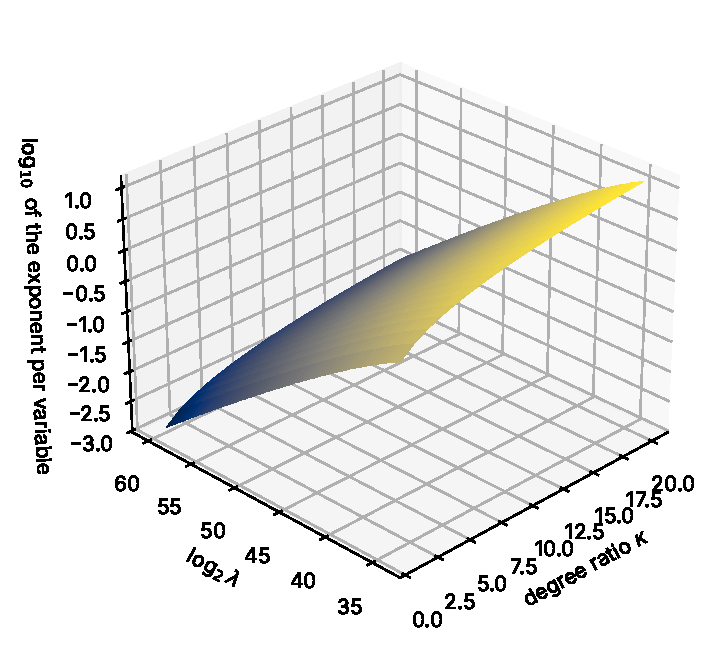
\includegraphics[width=0.78\textwidth]{figures/fig_costs}
\caption{The sum of the three costs of \eqref{eq:threecosts} per variable,
with the parameters \eqref{eq:params} for $\beta=2$, as a function of
$\lambda=\lceil\log n\rceil$ and of the degree ratio $\kappa$, drawn where the
hypotheses $r\ge2$ and $6R\le Q$ of Lemma~\ref{lem:params} hold. The surface
falls like $\nu^2/\sqrt\lambda$ in $\lambda$ and grows linearly in $\kappa$.}
\label{fig:costs}
\end{figure}

\subsection{Choosing the parameters}
The exponent of the routine depends on the three quantities of
\eqref{eq:threecosts}. The following choice bounds all three when $b$ and $w$
are bounded by a fixed power of $\log n$.

\begin{lemma}[Parameters]\label{lem:params}
Fix an integer $\beta\ge1$. Let $n\ge20$, $\lambda=\lceil\log n\rceil$,
$\nu=\lceil\log\lambda\rceil$, and suppose $b,w\le\lambda^{\beta}$ and
$n\le M\le bn$. For all sufficiently large $n$ the parameters
\begin{equation}\label{eq:params}
  r=\Bigl\lfloor\frac{\sqrt\lambda}{\nu^2}\Bigr\rfloor,\quad
  Q=\Bigl\lfloor\frac{\lambda}{128\nu}\Bigr\rfloor,\quad
  R=(\beta+3)\lceil\sqrt\lambda\rceil,\quad
  \tau=\frac1{r\lambda},\quad \epsilon=\frac1{br^2\lambda},\quad D=r^{2Q},
\end{equation}
with the interval $\mathcal J$ specified in the proof, satisfy the hypotheses of
Lemma~\ref{lem:complete}; moreover $R\ge32$, $6R\le Q$, $D\le2^{\lambda/128}$, and
\begin{equation}\label{eq:costs}
  \frac RQ\log\frac{2Q}R+\tau\log(2D+1)+\frac1r=O_\beta\Bigl(\frac{\nu^2}{\sqrt\lambda}\Bigr).
\end{equation}
Given $n,M,b,w$ the parameters can be computed and the hypotheses checked in
$\poly_\beta(\log n)$ bit operations, and for fixed $\beta$ only finitely many $n$
fail the checks.\footnote{Lemma 4.8 of \cite{OAI26}.}
\end{lemma}

\begin{proof}
For large $n$, $r=\Theta(\sqrt\lambda/\nu^2)$, $Q=\Theta(\lambda/\nu)$ and
$R=\Theta_\beta(\sqrt\lambda)$; so eventually $r\ge2$, $R\ge32$ and $6R\le Q$.
Since $\log r\le\nu/2$, $\log D=2Q\log r\le\lambda/128$. The balance inequalities
\eqref{eq:balance} hold for large $n$: $2(b+w)D^2\le4\lambda^\beta2^{\lambda/64}\le n\le M$
and $2Qr^2\le n$, because $Q,r$ are bounded by fixed powers of $\lambda$ while
$n>2^{\lambda-1}$. Put
\[
  \mu=\frac{Q(r-1)}{2r},\qquad A_0=\Bigl\lfloor\mu-\frac{R-1}2\Bigr\rfloor,\qquad
  \mathcal J=\{A_0,\dots,A_0+R-1\}.
\]
Then $Q/4\le\mu\le Q/2$, and since $R\le Q/6$ the interval lies in
$\{0,\dots,Q\}$; its centre is within one of $\mu$, and $R\ge32$ makes it contain
every integer within $R/4$ of $\mu$. For $\mathsf W\sim\Bin(Q,\frac{r-1}{2r})$,
Hoeffding's inequality \eqref{eq:hoeffding} with $s=R/4$ gives
\[
  \Pr[\mathsf W\notin\mathcal J]\le2e^{-R^2/(8Q)}\le2e^{-16(\beta+3)^2\nu}
  \le2^{-(\beta+2)\nu}\le\lambda^{-(\beta+2)}\le\frac1{br^2\lambda},
\]
using $R^2/(8Q)\ge(\beta+3)^2\lambda\cdot128\nu/(8\lambda)=16(\beta+3)^2\nu$,
$b\le\lambda^\beta$ and $r^2\le\lambda$. This is \eqref{eq:tailreq} with
$\epsilon=\tau/(rb)$, and $0<\tau\le1/2$ once $r\ge2$. Finally
$R/Q=O_\beta(\nu/\sqrt\lambda)$, $\log(2Q/R)=O(\nu)$ and
$\tau\log(2D+1)=O(1/r)$, while $1/r=O(\nu^2/\sqrt\lambda)$, which proves
\eqref{eq:costs}.

For the computation, $\lambda$ is the least integer with $n\le2^\lambda$ and $\nu$
the least with $\lambda\le2^\nu$; $r$ is the largest integer with
$r^2\nu^4\le\lambda$, $Q$ is an integer division, and $\lceil\sqrt\lambda\rceil$
comes from an integer square root. The algorithm reports failure if $r<2$ or
$Q\le R$; otherwise it forms $\tau,\epsilon,D$ and the endpoints of $\mathcal J$
in rational arithmetic and checks $\mathcal J\subseteq\{0,\dots,Q\}$,
\eqref{eq:balance}, $R\ge32$, $6R\le Q$, and \eqref{eq:tailreq}, whose left side
has denominator $(2r)^Q$ and is an exact rational computation. All of this takes
$\poly_\beta(\log n)$ bit operations, and the estimates above show that every check
passes for large $n$.
\end{proof}

%%==================================================================
\section{Weighted counting in subexponential time}\label{sec:weighted}
%%==================================================================

\subsection{Bounded occurrences}
We first state the outcome of Sections \ref{sec:routine} and \ref{sec:design}
for a factor system in which every variable occurs in few factors.

\begin{theorem}[Bounded occurrences]\label{thm:bounded-occ}
Fix an integer $\beta\ge1$. There are $n_0=n_0(\beta)$ and an absolute constant
$C_0$ with the following property. Let $\A$ be a commutative $\Q$-algebra, let
$n\ge n_0$, and let a factor system on $n$ variables have largest scope $w$,
largest occurrence number $b$ and total degree $d$ with
\[
  w\le\lambda^{\beta},\qquad b\le\lambda^{\beta},\qquad d\le\kappa n
\]
for some $\kappa\ge1$. Then $Z$ in \eqref{eq:Z} can be computed deterministically
with at most
\begin{equation}\label{eq:boundedocc}
  |\F|\,\poly(n)\,2^{\,C_0(\kappa+1)(\beta+3)\,n\nu^2/\sqrt\lambda}
\end{equation}
operations in $\A$, evaluations of factors at inputs in $\Q[z]/(z^{J})$ with
$J\le\kappa n$, and bit operations on rational numbers, using polynomially many
elements of $\A$ and polynomially many bits of storage in addition to the
factors' own.
\end{theorem}

\begin{proof}
Adjoin the constant-one factors of Section~\ref{sec:design} so that
\eqref{eq:nMb} holds; $b$ grows by at most one and $d$ is unchanged, and we may
take $n_0$ so large that $\lambda^\beta+1\le\lambda^{\beta+1}$ is not needed:
replace $\beta$ by $\beta+1$ in Lemma~\ref{lem:params} if $b$ was exactly
$\lambda^\beta$, which changes only the constants. Choose the parameters
\eqref{eq:params} by Lemma~\ref{lem:params}, which for $n\ge n_0(\beta)$
satisfy the hypotheses of Lemma~\ref{lem:complete}; construct the design in
polynomial time by that lemma; and run the routine of
Proposition~\ref{prop:routine}. The degree bound \eqref{eq:degbound} holds with
$d\le\kappa n$, so $d_H\le\kappa nR$, $q\le\kappa nR/Q$ and $J\le q+1\le\kappa n$
because $R<Q$. By \eqref{eq:logCq},
\[
  \log C_q\le\kappa n\frac RQ\log\frac QR+\frac{3nR}{Q}
  \le(\kappa+1)\,n\,\frac{R}{Q}\log\frac{2Q}{R}\cdot 3 .
\]
With the parameters \eqref{eq:params} and $n$ large, $R/Q\le 300(\beta+3)\nu/\sqrt\lambda$
and $\log(2Q/R)\le\nu$, while $\tau\log(2D+1)\le 1/r$ and
$1/r\le 2\nu^2/\sqrt\lambda$. Hence the logarithm of the vector count
\eqref{eq:routinecost} is at most
\[
  \log(2Qr)+900(\kappa+1)(\beta+3)\frac{n\nu^2}{\sqrt\lambda}+\frac{4n\nu^2}{\sqrt\lambda}
  \le \log(2Qr)+C_0(\kappa+1)(\beta+3)\frac{n\nu^2}{\sqrt\lambda}
\]
with $C_0=904$, and each vector costs at most $|\F|$ factor evaluations and
polynomially many further operations. The storage bound is that of
Proposition~\ref{prop:routine}.
\end{proof}

\subsection{Branching on frequent variables}
A sparse system may still contain variables occurring in many factors. Fixing
them removes the obstacle at a cost that is negligible against
\eqref{eq:boundedocc}.

\begin{lemma}[Frequent variables]\label{lem:frequent}
Let a factor system on $n\ge 20$ variables have $|\F|\le cn$ factors, each of
scope at most $k$, and let $V_{\mathrm{hi}}=\{v\in[n]:\#\{f:v\in I_f\}>ck\lambda\}$.
Then $|V_{\mathrm{hi}}|<n/\lambda$. For every assignment
$y\in\{0,1\}^{V_{\mathrm{hi}}}$ the system obtained by substituting $x_v=y_v$ for
$v\in V_{\mathrm{hi}}$ is a factor system on the $n'=n-|V_{\mathrm{hi}}|$
remaining variables, with at most $cn$ factors, scopes at most $k$, occurrence
numbers at most $ck\lambda$ and total degree at most $d$, and
\begin{equation}\label{eq:branchsum}
  Z=\sum_{y\in\{0,1\}^{V_{\mathrm{hi}}}}Z_y ,
\end{equation}
where $Z_y$ is the sum \eqref{eq:Z} of the substituted system.
\end{lemma}

\begin{proof}
The incidences number $M\le k|\F|\le ckn$, so fewer than $ckn/(ck\lambda)=n/\lambda$
variables occur more than $ck\lambda$ times. Substituting values for the variables
in $V_{\mathrm{hi}}$ restricts each $\Phi_f$ to a polynomial in the remaining
variables of its scope, of no larger degree; the scopes shrink and the occurrence
numbers of the remaining variables are unchanged, hence at most $ck\lambda$.
Splitting the sum over $\{0,1\}^n$ according to $x|_{V_{\mathrm{hi}}}$ gives
\eqref{eq:branchsum}.
\end{proof}

\subsection{The weighted counting theorem}
\begin{theorem}[Weighted counting]\label{thm:weighted}
Fix integers $k\ge1$ and $c\ge1$. There is a deterministic algorithm that, given
a factor system on $n\ge 20$ variables with at most $cn$ factors, each of scope at
most $k$ and with values in a commutative $\Q$-algebra $\A$, computes
\[
  Z=\sum_{x\in\{0,1\}^n}\prod_{f\in\F}\Phi_f\bigl((x_v)_{v\in I_f}\bigr)
\]
with
\begin{equation}\label{eq:weightedtime}
  \poly(n)\,2^{\,O_{k,c}(\rhon(n))},\qquad \rhon(n)=\frac{n(\log\log n)^2}{\sqrt{\log n}},
\end{equation}
operations in $\A$ and evaluations of the factors at inputs in $\Q[z]/(z^J)$,
$J\le ckn$, together with polynomially many bit operations on rationals, and
polynomially many elements of $\A$ and bits of storage. The implied constant
depends only on $k$ and $c$.
\end{theorem}

\begin{proof}
Let $n_0=n_0(2)$ be the threshold of Theorem~\ref{thm:bounded-occ} with $\beta=2$,
enlarged so that $ck\lambda\le(\lambda-1)^2$ and $k\le(\lambda-1)^2$ for
$n\ge n_0$. If $n<2n_0$, enumerate the cube directly: $2^{n}\le 2^{2n_0}$ is a
constant depending on $k,c$. Otherwise $n\ge 2n_0$; apply Lemma~\ref{lem:frequent}. For each
of the fewer than $2^{n/\lambda}$ assignments $y$, the substituted system has
$n'\ge n-n/\lambda\ge n/2\ge n_0$ variables, scopes at most $k\le\lambda'^{2}$,
occurrences at most $ck\lambda\le\lambda'^{2}$, where $\lambda'=\lceil\log n'\rceil\ge\lambda-1$,
and total degree $d\le kcn\le 2ck\,n'$. Theorem~\ref{thm:bounded-occ} with
$\beta=2$ and $\kappa=2ck$ computes $Z_y$ with
$|\F|\poly(n)2^{5C_0(2ck+1)n'\nu'^2/\sqrt{\lambda'}}$ operations, and
$n'\nu'^2/\sqrt{\lambda'}\le 2n\nu^2/\sqrt\lambda$ for large $n$. Summing the
$Z_y$ costs one operation each. The total is
\[
  2^{n/\lambda}\cdot cn\,\poly(n)\,2^{10C_0(2ck+1)n\nu^2/\sqrt\lambda}
  =\poly(n)\,2^{O_{k,c}(n\nu^2/\sqrt\lambda)},
\]
since $n/\lambda\le n\nu^2/\sqrt\lambda$, and $n\nu^2/\sqrt\lambda=\Theta(\rhon(n))$.
The space bound follows from Theorem~\ref{thm:bounded-occ} because the branches
are processed one after the other.
\end{proof}

\begin{remark}
For $\A=\Q$ and $\Phi_f$ the satisfaction indicator of a clause, $Z$ is the number
of satisfying assignments and the theorem is the sparse case of
\oai{}'s Theorem 1.1, with the exponent $\rhon(n)$ of their Proposition 6.4 in
place of $n\log\log n/\sqrt{\log n}$. The dense case, and the better exponent, use
their Sections 5, 6 and Appendices A and B, which are not reproduced here; the
dense case is recovered in Section~\ref{sec:snp} from the published
sparsification lemma, with a weaker time bound.
\end{remark}

\subsection{Bit complexity over truncated polynomial rings}
\begin{lemma}[Bit complexity]\label{lem:bits}
In the situation of Theorem~\ref{thm:bounded-occ}, of Theorem~\ref{thm:explicit} or of Theorem~\ref{thm:weighted},
with $|\F|$ factors of scope at most $k$ and total degree $d$, let $\A$ be one of the algebras
$\A_N=\Q[W]/(W^N)$, $\A_{N_1,\dots,N_s}$ of dimension $N=N_1\cdots N_s$, or
$\Q[W]/(W^N-1)$, and suppose every coefficient of every $\Phi_f$, as a polynomial
in the $Y_v$ with coefficients in $\A$, is a polynomial in the generators with
integer coefficients of absolute value at most $2^{L}$. Then every rational number that the algorithm
forms has numerator and denominator of $\poly(n,|\F|,k,N,L)$ bits; hence the operation
counts of those theorems turn into bounds on bit operations after multiplication
by a polynomial in $n$, $|\F|$, $k$, $N$ and $L$, and the space stays polynomial.
\end{lemma}

\begin{proof}
All numbers arise in the following places. (a) The rows: by \ref{D5},
$d_{\mathrm{den}}\PP_{f,v}$ has integer coefficients of $O(Q\log Q+\log D)=O(\lambda)$
bits, and the values $\ip{\PP_{f,v}(t)}{x}$ for Boolean $x$ and the coefficients of
$\ip{\Delta\PP_{f,v}(z)}{\mathbf 1_U}$ are sums of at most $n$ such coefficients
times powers $t^{i}\le Q^{R}$, hence rationals with denominator
$d_{\mathrm{den}}$ and numerators of $O(\lambda+R\log Q+\log n)=O(\lambda)$ bits.
(b) A factor evaluation: $\Phi_f$ has degree at most $k$, so its value at inputs
in $\Q[z]/(z^J)$ with the bounds of (a) is an element of $\A[z]/(z^J)$ with
denominator $d_{\mathrm{den}}^{k}$ and numerators of $O(L+k\lambda+k\log J)$ bits.
(c) A group product is a product of at most $|\F|$ factor values in
$\A[z]/(z^J)$; the number of monomials contributing to one coefficient is at
most $(NJ)^{|\F|}$, so the product has denominator $d_{\mathrm{den}}^{k|\F|}$ and
numerators of $O(|\F|(L+k\lambda+k\log(NJ)))$ bits. (d) The sums
\eqref{eq:Sigma}, \eqref{eq:ZE} and \eqref{eq:Htsum} add at most
$2^{n}\cdot 3^{n}\cdot(2D+1)^{2\tau n}$ terms with a common denominator, adding
$O(n+n\log(2D+1))=O(n\lambda)$ bits to the numerators. (e) Hermite interpolation
solves a $QJ\times QJ$ rational system with entries of $O(QJ\log(QJ))$ bits and
right-hand sides as in (d); by Cramer's rule the solution has denominator and
numerators of $\poly(QJ)\cdot O(n\lambda+|\F|(L+k\lambda+k\log(NJ)))$ bits. Since
$Q,\lambda=O(\log n)$ and $J\le d+1\le k|\F|+1$, all bit lengths are
$\poly(n,|\F|,k,N,L)$, and each
operation in $\A$ costs $O(N^2)$ operations on such rationals. The count of
monomials in (c) used only that a product of two basis elements of $\A$ is a
basis element or zero, which holds in all three algebras.
The case $\A=\Q$ is $N=1$.
\end{proof}

%%==================================================================
\section{Profiles, optima and polynomials}\label{sec:applications}
%%==================================================================

This section draws the consequences of Theorem~\ref{thm:weighted} and of
Theorem~\ref{thm:bounded-occ}. The pattern is the same each time: a
combinatorial quantity is written as the sum \eqref{eq:Z} of a factor system
over a cube, the algebra is chosen so that the sum records what one wants to
know, and the two theorems are applied. The only place where something has to
be added to the summation routine is the independence polynomial of a graph
without any bound on the degrees, in Section~\ref{ssec:indep}, where a
branching rule reduces the general graph to graphs of small degree; the cost of
the rule is bounded by an explicit induction.

\subsection{Profiles of sparse constraint systems}\label{ssec:profile}
A \emph{constraint system} on $n$ Boolean variables consists of constraints
$C_1,\dots,C_m$, where $C_f:\{0,1\}^{I_f}\to\{0,1\}$ is given by its truth
table on a scope $I_f\subseteq[n]$, together with nonnegative integer weights
$\omega_1,\dots,\omega_m$. For an assignment $x$ write
\[
  \sat_\omega(x)=\sum_{f:\,C_f(x|_{I_f})=1}\omega_f
\]
for the weight of the constraints it satisfies. The \emph{profile} of the
system is the sequence
\begin{equation}\label{eq:csprofile}
  p_j=\#\{x\in\{0,1\}^n:\sat_\omega(x)=j\},\qquad 0\le j\le\Omega_{\mathrm{tot}}=\sum_f\omega_f .
\end{equation}

\begin{theorem}[Profiles]\label{thm:profile}
Fix integers $k\ge1$ and $c\ge1$. There is a deterministic algorithm that, given
a constraint system on $n\ge20$ variables with $m\le cn$ constraints of scope at
most $k$ and weights $\omega_f\le\Omega$, computes the whole profile
\eqref{eq:csprofile} in time $\poly(n,\Omega)\,2^{O_{k,c}(\rhon(n))}$ and
polynomial space.
\end{theorem}

\begin{proof}
Let $N=1+\Omega_{\mathrm{tot}}\le 1+cn\Omega$ and $\A=\A_N$. For each $f$ let
$\Phi_f$ be the multilinear extension \eqref{eq:multilinear} of the function
$\phi_f(x)=W^{\omega_f C_f(x)}$ on $\{0,1\}^{I_f}$; its coefficients are the
polynomials $\sum_{U\subseteq S}(-1)^{|S|-|U|}\phi_f(\mathbf 1_U)$, each a sum of
at most $2^k$ monomials $\pm W^{j}$, so they are polynomials in $W$ with integer
coefficients of absolute value at most $2^k$. The system $(\Phi_f)$ is a factor
system with at most $cn$ factors of scope at most $k$, and by
\eqref{eq:profile}, since $\sum_f\omega_fC_f(x)=\sat_\omega(x)\le\Omega_{\mathrm{tot}}<N$,
\[
  Z=\sum_{x}\prod_f W^{\omega_fC_f(x|_{I_f})}=\sum_{j}p_jW^{j}
\]
with no term lost to the truncation. Theorem~\ref{thm:weighted} computes $Z$
with $\poly(n)2^{O_{k,c}(\rhon(n))}$ operations in $\A_N$ and factor
evaluations, and Lemma~\ref{lem:bits} with $L=k$ bounds the bit lengths by
$\poly(n,N)$, so the bit cost is $\poly(n,\Omega)2^{O_{k,c}(\rhon(n))}$. The
coefficients $p_j$ are read off from $Z$.
\end{proof}

The profile contains, besides the optimum, every quantity that depends only on
the distribution of the objective over the cube.

\begin{corollary}[Max-$k$-SAT]\label{cor:maxsat}
Fix $k,c\ge1$. Given a $k$-CNF formula with $n$ variables and $m\le cn$ clauses
with integer weights in $[0,\Omega]$, the following are computed deterministically
in time $\poly(n,\Omega)2^{O_{k,c}(\rhon(n))}$: the maximum weight of
simultaneously satisfiable clauses, the number of assignments attaining it, the
minimum such weight, and for every $j$ the number of assignments satisfying
clauses of total weight exactly $j$. In particular Max-$k$-SAT, Min-$k$-SAT and
weighted Max-$k$-SAT with polynomially bounded weights are solved exactly in time
$2^{o(n)}$ on instances with $O(n)$ clauses, and the number of optimal
assignments is counted.
\end{corollary}

\begin{proof}
A clause is a constraint whose truth table is the disjunction of its literals.
Apply Theorem~\ref{thm:profile}; the maximum is the largest $j$ with $p_j>0$,
the minimum the smallest, and $p_j$ is the required count.
\end{proof}

The Hamming weight of an assignment is itself a sum of local weights, one per
variable, so the profile may be taken with respect to it.

\begin{corollary}[Satisfying assignments of each weight]\label{cor:hamming}
Fix $k,c\ge1$. Given a $k$-CNF formula with $n$ variables and $m\le cn$ clauses,
the numbers
\[
  s_i=\#\{x:\ x\text{ satisfies the formula and has exactly $i$ ones}\},\qquad 0\le i\le n,
\]
are computed deterministically in time $\poly(n)2^{O_{k,c}(\rhon(n))}$. Hence the
satisfying assignment with the fewest, or the most, ones is found and counted
within the same time.
\end{corollary}

\begin{proof}
Take $\A=\A_{n+1}$. For each clause $f$ let $\Phi_f$ be the multilinear extension
of its satisfaction indicator, with coefficients in $\{0,\pm1\}\subseteq\Q$, and
for each variable $v$ add the factor $\Phi_v=1+(W-1)Y_v$ of scope $\{v\}$,
the multilinear extension of $W^{x_v}$. The system has at most $(c+1)n$ factors
of scope at most $k$, and its sum is
$Z=\sum_x[\text{$x$ satisfies the formula}]\,W^{|x|}=\sum_is_iW^i$, where $|x|$
is the number of ones. Theorem~\ref{thm:weighted} and Lemma~\ref{lem:bits}
with $N=n+1$, $L=1$ give the time bound. A satisfying assignment of a prescribed
weight $i$ with $s_i>0$ is then found by the usual self-reduction: fix the first
variable to $0$ and to $1$, recompute the profiles of the two restricted
formulas, which are again sparse $k$-CNF formulas, keep a value for which the
coefficient of $W^{i}$ or $W^{i-1}$ is positive, and continue; this multiplies
the time by at most $2n$.
\end{proof}

The next corollary uses an algebra in two variables, one recording the cut and
one the size of a side.

\begin{corollary}[Max-Cut and bisections]\label{cor:maxcut}
Fix $c\ge1$. Given a graph $G$ with $n$ vertices and $m\le cn$ edges with integer
weights in $[0,\Omega]$, the numbers
\[
  q_{i,j}=\#\{S\subseteq V(G):\ |S|=i,\ \text{the edges between $S$ and $V\setminus S$ have total weight $j$}\}
\]
are computed for all $i$ and $j$ in deterministic time
$\poly(n,\Omega)2^{O_c(\rhon(n))}$. In particular the maximum cut, the maximum
and the minimum bisection, with the number of optimal solutions of each, are
computed exactly in time $2^{o(n)}$ on graphs with $O(n)$ edges.
\end{corollary}

\begin{proof}
Let $N_1=1+\sum_e\omega_e\le1+cn\Omega$ and $N_2=n+1$, and let
$\A=\A_{N_1,N_2}=\Q[W,U]/(W^{N_1},U^{N_2})$. Encode $S$ by $x\in\{0,1\}^n$. For an
edge $e=\{u,v\}$ take the multilinear extension of $W^{\omega_e[x_u\ne x_v]}$,
which is $1+(W^{\omega_e}-1)(Y_u+Y_v-2Y_uY_v)$, and for each vertex $v$ the
factor $1+(U-1)Y_v$. There are at most $(c+1)n$ factors of scope at most $2$,
with coefficients that are polynomials in $W$ and $U$ with integer coefficients
of absolute value at most $2$. The sum is
$Z=\sum_x W^{\mathrm{cut}(x)}U^{|x|}=\sum_{i,j}q_{i,j}W^{j}U^{i}$, and no term is
truncated. Theorem~\ref{thm:weighted} and Lemma~\ref{lem:bits} with
$N=N_1N_2$ and $L=1$ give the bound. The maximum cut is the largest $j$ with
$\sum_iq_{i,j}>0$, the maximum bisection the largest $j$ with
$q_{\lfloor n/2\rfloor,j}>0$, the minimum bisection the smallest such $j$, and
the counts are the coefficients.
\end{proof}

\begin{figure}[t]
\centering
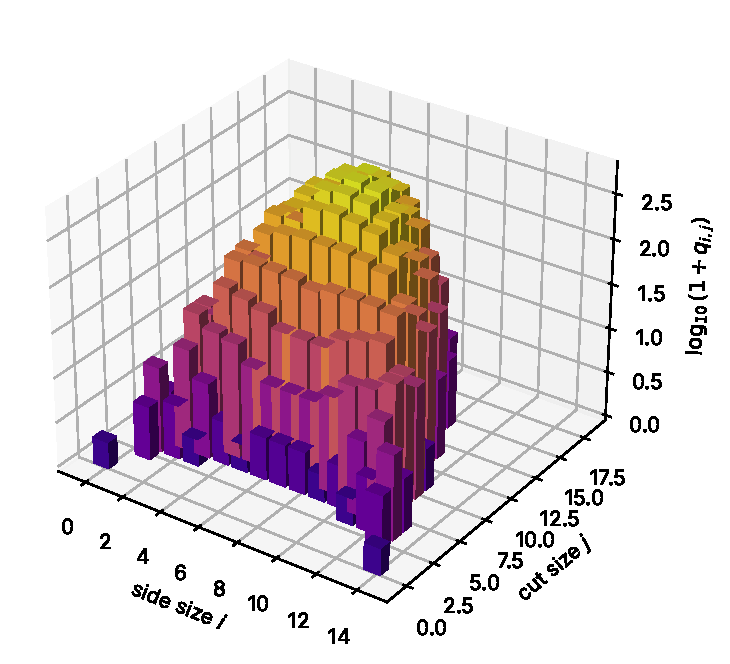
\includegraphics[width=0.74\textwidth]{figures/fig_profile}
\caption{The array $q_{i,j}$ of Corollary~\ref{cor:maxcut} for a graph with
$14$ vertices and $21$ edges, a Hamilton cycle with seven chords, computed
directly from the $2^{14}$ subsets; the height is $\log_{10}(1+q_{i,j})$. The
algorithm returns the whole array as one element of $\Q[W,U]/(W^{22},U^{15})$;
its maximum cut and its maximum bisection are both $18$.}
\label{fig:profile}
\end{figure}

\begin{remark}
The best exact algorithm for Max-Cut on general graphs runs in time
$2^{\omega n/3}\le2^{0.792n}$ \cite{Wil05}, and the exact algorithms for sparse
Max-Cut run in time $2^{\Theta(m)}$ \cite{SS09}; on graphs with $m=O(n)$ edges
both are exponential in $n$. The proof of \oai{}'s Corollary 1.2 contains a
circuit encoding that, combined with their Theorem 1.1, also yields the exact
optimum of a sparse Max-$k$-SAT or Max-Cut instance in time $2^{o(n)}$, by a
binary search over the threshold; that route handles the unweighted objective.
The algebra $\A_N$ handles integer weights up to $\Omega$ at a cost polynomial in
$\Omega$, which a circuit encoding cannot do without introducing $\Theta(n\log\Omega)$
auxiliary variables.
\end{remark}

\subsection{The independence polynomial of every graph}\label{ssec:indep}
Let $G$ be a graph with vertex set $V$, $|V|=n$, and let $\omega:V\to\{0,1,\dots\}$
be integer vertex weights. The weighted independence polynomial is
\begin{equation}\label{eq:indeppoly}
  I_\omega(G;W)=\sum_{S\subseteq V\text{ independent}}W^{\omega(S)},\qquad \omega(S)=\sum_{v\in S}\omega_v ,
\end{equation}
and $I(G;W)=I_{\mathbf 1}(G;W)$ is the independence polynomial. For a vertex $v$
write $N[v]$ for its closed neighbourhood and $G-X$ for the graph induced on
$V\setminus X$. Every independent set either avoids $v$ or contains $v$ and
avoids $N[v]$, so
\begin{equation}\label{eq:indeprec}
  I_\omega(G;W)=I_\omega(G-v;W)+W^{\omega_v}\,I_\omega(G-N[v];W).
\end{equation}

\begin{lemma}[Forcing branching]\label{lem:branch}
Let $b\ge2$ be an integer and $G$ a weighted graph with $n$ vertices. There is a
binary tree, computable in time $\poly(n)$ per node, whose leaves $\ell$ carry
induced subgraphs $H_\ell$ of $G$ of maximum degree at most $b$ and integers
$s_\ell\ge0$ such that
\begin{equation}\label{eq:branchexp}
  I_\omega(G;W)=\sum_{\ell}W^{s_\ell}\,I_\omega(H_\ell;W),
\end{equation}
and the number of leaves is at most
\begin{equation}\label{eq:leaves}
  \Bigl(1+\frac{2\ln(b+2)}{b+1}\Bigr)^{n}.
\end{equation}
\end{lemma}

\begin{proof}
Build the tree from the root $(G,0)$. At a node $(H,s)$ in which some vertex $v$
has degree greater than $b$ in $H$, attach the two children $(H-v,s)$ and
$(H-N_H[v],s+\omega_v)$; by \eqref{eq:indeprec} the sum
$\sum W^{s}I_\omega(H;W)$ over the nodes of any antichain that cuts every
root-to-leaf path is the same, and it equals $I_\omega(G;W)$ at the root. A node
in which every vertex has degree at most $b$ is a leaf. This gives
\eqref{eq:branchexp}, and each node is processed in polynomial time.

Let $L(n)$ be the largest number of leaves of such a tree over all weighted graphs
with at most $n$ vertices, so that $L$ is nondecreasing and $L(n)=1$ for
$n\le b+1$, because a graph with at most $b+1$ vertices has maximum degree at
most $b$. If $v$ has degree at least $b+1$ then $H-v$ has $n-1$ vertices and
$H-N_H[v]$ at most $n-b-2$, so
\[
  L(n)\le L(n-1)+L(n-b-2)\qquad(n\ge b+2),
\]
with $L(j)=1$ for $j\le b+1$, including $j\le0$. Put $\varepsilon=2\ln(b+2)/(b+1)$.
We claim $L(n)\le(1+\varepsilon)^n$ for all $n\ge0$. This holds for $n\le b+1$.
For $n\ge b+2$, by induction,
\[
  L(n)\le(1+\varepsilon)^{n-1}+(1+\varepsilon)^{n-b-2}
  =(1+\varepsilon)^{n-b-2}\bigl((1+\varepsilon)^{b+1}+1\bigr),
\]
and the right side is at most $(1+\varepsilon)^{n}$ exactly when
$\varepsilon(1+\varepsilon)^{b+1}\ge1$. Now $b\ge2$ gives
$2\ln(b+2)\le b+1$, since this holds at $b=2$ ($2\ln4<3$) and the difference
$b+1-2\ln(b+2)$ increases with $b$; so $\varepsilon\le1$, and for
$0\le\varepsilon\le1$ one has $\ln(1+\varepsilon)\ge\varepsilon-\varepsilon^2/2\ge\varepsilon/2$.
Therefore
\[
  (1+\varepsilon)^{b+1}\ge e^{(b+1)\varepsilon/2}=e^{\ln(b+2)}=b+2,
  \qquad
  \varepsilon(1+\varepsilon)^{b+1}\ge\frac{2\ln(b+2)}{b+1}(b+2)\ge2\ln4>1 .
\]
This proves the claim, and \eqref{eq:leaves} follows.
\end{proof}

\begin{figure}[t]
\centering
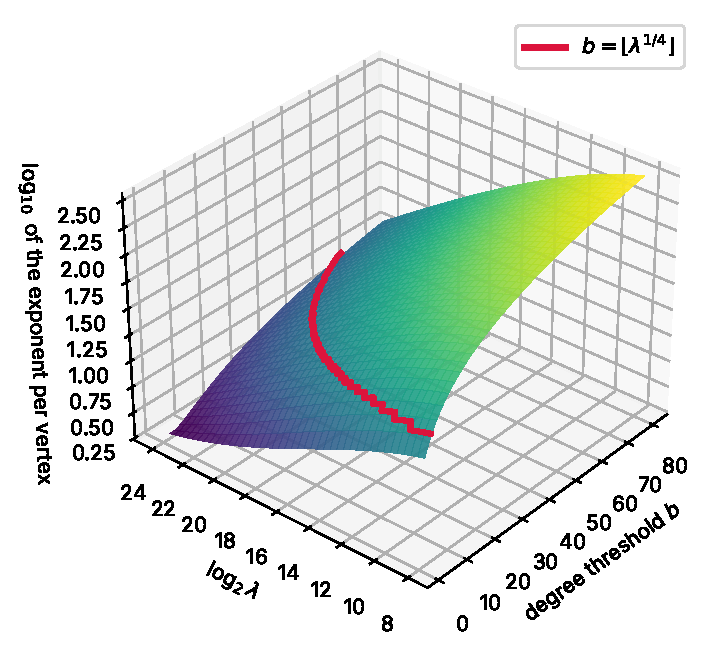
\includegraphics[width=0.78\textwidth]{figures/fig_branch}
\caption{The two costs of the proof of Theorem~\ref{thm:indep} per vertex, in
$\log_{10}$, with the constant $C_0$ omitted: the leaf count
$2\ln(b+2)/(b+1)$ of Lemma~\ref{lem:branch} and the leaf cost
$(b+2)\nu^2/\sqrt\lambda$ of Theorem~\ref{thm:bounded-occ}, as a function of
the degree threshold $b$ and of $\lambda$; the curve marks the choice
$b=\lfloor\lambda^{1/4}\rfloor$ of the proof.}
\label{fig:branch}
\end{figure}

\begin{theorem}[Independence polynomial]\label{thm:indep}
There is a deterministic algorithm that, given a graph $G$ with $n$ vertices and
integer vertex weights in $[0,\Omega]$, computes the weighted independence
polynomial $I_\omega(G;W)$ in time
\[
  \poly(n,\Omega)\,2^{O(n(\log\log n)^2/(\log n)^{1/4})}
\]
and polynomial space. No condition is placed on the graph.
\end{theorem}

\begin{proof}
Let $n_0=n_0(1)$ be the threshold of Theorem~\ref{thm:bounded-occ} with $\beta=1$
and let $n_1\ge n_0^2$ be so large that for $n\ge n_1$ the following hold, with
$\lambda=\lceil\log n\rceil$ and $b=\lfloor\lambda^{1/4}\rfloor$: $b\ge2$,
$\lambda^{1/4}+1\le\lambda/2-1$, and $\lambda/2-1\ge\lambda/3$. For $n<n_1$
compute $I_\omega(G;W)$ by listing the $2^{n}<2^{n_1}$ subsets, a constant. For
$n\ge n_1$ apply Lemma~\ref{lem:branch} with this $b$ and compute
$I_\omega(H_\ell;W)$ at each leaf as follows.

If $H=H_\ell$ has $n_H<\sqrt n$ vertices, list its subsets; this costs
$2^{\sqrt n}\poly(n,\Omega)$. Otherwise $n_H\ge\sqrt n$, so
$\lambda_H=\lceil\log n_H\rceil\ge\lambda/2-1\ge\lambda/3$ and $n_H\ge n_0$. Take
$\A=\A_N$ with $N=1+\sum_v\omega_v\le1+n\Omega$, and the factor system on the
$n_H$ variables $x_v$, $v\in V(H)$, with the factor $1-Y_uY_v$ for each edge
$uv$ of $H$ and the factor $1+(W^{\omega_v}-1)Y_v$ for each vertex $v$. The
edge factor is the multilinear extension of the indicator that $u$ and $v$ are
not both chosen, and the vertex factor that of $W^{\omega_vx_v}$, so the sum
\eqref{eq:Z} is $I_\omega(H;W)$, with no term truncated. Each variable occurs in
at most $\deg_H(v)+1\le b+1\le\lambda^{1/4}+1\le\lambda_H$ factors, the scopes are
at most $2\le\lambda_H$, and the total degree is
$d=2|E(H)|+n_H\le(b+1)n_H$. Theorem~\ref{thm:bounded-occ} with $\beta=1$ and
$\kappa=b+1$ applies and computes $I_\omega(H;W)$ with
\[
  |\F|\,\poly(n_H)\,2^{\,4C_0(b+2)\,n_H\nu_H^2/\sqrt{\lambda_H}}
  \le\poly(n)\,2^{\,4C_0(\lambda^{1/4}+2)\,n\nu^2\sqrt{3/\lambda}}
  =2^{O(n\nu^2/\lambda^{1/4})}
\]
operations in $\A_N$, using $\nu_H\le\nu$ and $\lambda_H\ge\lambda/3$;
Lemma~\ref{lem:bits} with $|\F|\le(b+1)n$, $k=2$, $L=1$ turns this into
$\poly(n,\Omega)2^{O(n\nu^2/\lambda^{1/4})}$ bit operations.

By \eqref{eq:leaves} the tree has at most $(1+\varepsilon)^n\le e^{\varepsilon n}$
leaves with $\varepsilon=2\ln(b+2)/(b+1)\le 4\ln\lambda/\lambda^{1/4}=O(\nu/\lambda^{1/4})$,
hence at most $2^{O(n\nu/\lambda^{1/4})}$ leaves and fewer internal nodes, each
processed in polynomial time, and the leaf polynomials are combined by
\eqref{eq:branchexp} with one multiplication by a power of $W$ and one addition
in $\A_N$ per leaf. The tree is traversed depth first, so only one root-to-leaf
path of length at most $n$ is stored at a time, and the space is polynomial. The
total time is
\[
  2^{O(n\nu/\lambda^{1/4})}\cdot\bigl(2^{\sqrt n}+2^{O(n\nu^2/\lambda^{1/4})}\bigr)\poly(n,\Omega)
  =\poly(n,\Omega)\,2^{O(n\nu^2/\lambda^{1/4})},
\]
and $n\nu^2/\lambda^{1/4}=\Theta(n(\log\log n)^2/(\log n)^{1/4})$.
\end{proof}

\begin{corollary}\label{cor:indep}
Each of the following is computed deterministically, for every graph $G$ on $n$
vertices, in time $2^{O(n(\log\log n)^2/(\log n)^{1/4})}$: the independence
number $\alpha(G)$ and the number of maximum independent sets; the number of
independent sets of each size, hence the partition function of the hard-core
model at every activity; the clique number $\omega(G)$ and the number of maximum
cliques; the vertex cover number $\tau(G)$ and the number of minimum vertex
covers; and, for integer weights in $[0,\Omega]$, the maximum weight of an
independent set and the number of independent sets of that weight, with a factor
$\poly(\Omega)$ in the time.
\end{corollary}

\begin{proof}
$\alpha(G)$ is the degree of $I(G;W)$, its leading coefficient counts the maximum
independent sets, and the coefficient of $W^{i}$ counts the independent sets of
size $i$; the hard-core partition function at activity $z$ is $I(G;z)$. The
cliques of $G$ are the independent sets of the complement, to which
Theorem~\ref{thm:indep} applies without restriction. The vertex covers are the
complements of the independent sets, so $\tau(G)=n-\alpha(G)$ and the minimum
vertex covers are counted by the same leading coefficient. The weighted
statements read the degree and the leading coefficient of $I_\omega(G;W)$.
\end{proof}

\begin{remark}\label{rem:indep}
The fastest published exact algorithm for the maximum independent set runs in
time $2^{0.1996n}$ \cite{XN17}, and $2^{\Omega(n)}$ was a known consequence of
the exponential time hypothesis. \oai{}'s Corollary 1.3 gives the number of
independent sets of every graph in time $2^{o(n)}$ through their Theorem 1.1 in
its general form, which handles formulas with $\Theta(n^2)$ clauses; that form,
combined with a linear-size threshold circuit for the number of chosen vertices,
also gives $\alpha(G)$ with the exponent $n\log\log n/\sqrt{\log n}$. The route
of Theorem~\ref{thm:indep} is different: it uses only the sparse routine
reproduced in Sections \ref{sec:routine} and \ref{sec:design}, reaches every
graph through the branching of Lemma~\ref{lem:branch}, and returns the whole
weighted polynomial. Its exponent is larger, by the factor
$(\log n)^{1/4}\log\log n$, which is the price of the branching.
\end{remark}

The branching of Lemma~\ref{lem:branch} records the weight of the chosen
vertices only through the monomial $W^{\omega_v}$ that multiplies the second
child, and its proof uses nothing else about that monomial. Several weights can
therefore be carried at once, with one generator for each, and a budget can be
placed on each of them. No restriction is placed on the graph.

\begin{theorem}[Independent sets under budgets]\label{thm:indepbudget}
Fix $s\ge0$. There is a deterministic algorithm that, given a graph $G$ with $n$
vertices and weight vectors $\omega^{(0)},\dots,\omega^{(s)}\in\{0,1,\dots,\Omega\}^{V}$,
computes the numbers
\[
  a(j_0,\dots,j_s)=\#\bigl\{S\subseteq V\text{ independent}:\ \omega^{(i)}(S)=j_i\ (0\le i\le s)\bigr\}
\]
for all tuples $(j_0,\dots,j_s)$ in time
\[
  \poly\bigl(n,(1+n\Omega)^{s+1}\bigr)\,2^{O(n(\log\log n)^2/(\log n)^{1/4})}
\]
and polynomial space, the implied constant depending only on $s$.
\end{theorem}

\begin{proof}
Put $N_i=1+\sum_v\omega^{(i)}_v\le1+n\Omega$ and $\A=\A_{N_0,\dots,N_s}$, of
dimension $N=N_0\cdots N_s\le(1+n\Omega)^{s+1}$, and for a vertex $v$ write
$\mathbf W^{v}=\prod_{i=0}^{s}W_i^{\omega^{(i)}_v}$, a basis monomial of $\A$ since
$\omega^{(i)}_v<N_i$. The
polynomial
\[
  I(G)=\sum_{S\text{ independent}}\ \prod_{v\in S}\mathbf W^{v}
  =\sum_{(j_0,\dots,j_s)}a(j_0,\dots,j_s)\,W_0^{j_0}\cdots W_s^{j_s}
\]
loses no term to the truncation, because $\omega^{(i)}(S)<N_i$ for every $S$.
It satisfies $I(G)=I(G-v)+\mathbf W^{v}\,I(G-N[v])$ for every vertex $v$, by the
argument for \eqref{eq:indeprec}. The construction of the tree in
Lemma~\ref{lem:branch} uses only this recursion, with the second child carrying
the product of the monomials $\mathbf W^{v}$ of the vertices fixed to $1$ on the
way, and the bound \eqref{eq:leaves} on the number of leaves uses only the
numbers of vertices removed. So the lemma holds verbatim for $I(G)$, with leaf
terms $\mathbf m_\ell\,I(H_\ell)$ in which $\mathbf m_\ell$ is a monomial.

At a leaf $H=H_\ell$ with $n_H\ge\sqrt n$ vertices take, as in the proof of
Theorem~\ref{thm:indep}, the factor $1-Y_uY_v$ for each edge $uv$ of $H$ and
the factor $1+(\mathbf W^{v}-1)Y_v$ for each vertex $v$, the multilinear
extension of $\prod_i W_i^{\omega^{(i)}_vx_v}$. The sum \eqref{eq:Z} of this
system is $I(H)$. The occurrence numbers, the scopes and the total degree are
those of the proof of Theorem~\ref{thm:indep}, since only the coefficient of
$Y_v$ in the vertex factors has changed, and that coefficient is a polynomial
in the generators with integer coefficients of absolute value at most $1$.
Theorem~\ref{thm:bounded-occ} with $\beta=1$ and $\kappa=b+1$ gives
$\poly(n)2^{O(n\nu^2/\lambda^{1/4})}$ operations in $\A$, and
Lemma~\ref{lem:bits} with $L=1$ turns them into
$\poly(n,N)2^{O(n\nu^2/\lambda^{1/4})}$ bit operations. Leaves with fewer than
$\sqrt n$ vertices are summed directly, each of the at most $2^{\sqrt n}$
subsets costing $\poly(n,N)$. The count of leaves, the depth-first traversal
and the final estimate are those of the proof of Theorem~\ref{thm:indep}, with
$\poly(n,\Omega)$ replaced by $\poly(n,N)$.
\end{proof}

The knapsack problem with a conflict graph \cite{PS09} asks for a set of items
of largest value whose total weight is within a capacity and which contains no
two items joined by an edge of a given graph. It contains the maximum
independent set, and with several capacities it contains the multidimensional
knapsack problem.

\begin{corollary}[Knapsack with an arbitrary conflict graph]\label{cor:knapsack}
Fix $s\ge1$. Given a graph $G$ on $n$ vertices, values $\omega^{(0)}_v$ and
weights $\omega^{(1)}_v,\dots,\omega^{(s)}_v$ in $[0,\Omega]$, and capacities
$B_1,\dots,B_s$, the largest value $\omega^{(0)}(S)$ of an independent set $S$
of $G$ with $\omega^{(i)}(S)\le B_i$ for $1\le i\le s$, and the number of
independent sets attaining it, are computed deterministically in time
$\poly(n,\Omega^{s+1})\,2^{O(n(\log\log n)^2/(\log n)^{1/4})}$. The same holds
with any of the inequalities replaced by equalities or by lower bounds, and
with independent sets replaced by cliques.
\end{corollary}

\begin{proof}
By Theorem~\ref{thm:indepbudget} compute all $a(j_0,\dots,j_s)$. The optimum is
the largest $j_0$ for which $\sum a(j_0,j_1,\dots,j_s)>0$, the sum taken over
the tuples with $j_i\le B_i$ for $1\le i\le s$, and that sum is the number of
optimal sets; it has at most $(1+n\Omega)^{s}$ terms. Other relations between
$j_i$ and $B_i$ change only the range of the sum. Cliques of $G$ are the
independent sets of its complement.
\end{proof}

\subsection{Vertex Cover in time $2^{o(k)}$}\label{ssec:vc}
The parameterised Vertex Cover problem asks, for a graph $G$ with $n$ vertices
and an integer $k$, whether $G$ has a vertex cover with at most $k$ vertices.
We use the kernel of Chen, Kanj and Jia \cite{CKJ01}, which rests on the theorem
of Nemhauser and Trotter \cite{NT75} on the half-integral relaxation of the
problem.

\begin{theorem}[Nemhauser and Trotter; Chen, Kanj and Jia]\label{thm:kernel}
There is a polynomial-time algorithm that, given a graph $G$ and an integer
$k\ge0$, either reports correctly that $G$ has no vertex cover with at most
$k$ vertices, or returns an induced subgraph $G'$ of $G$ with at most $2k$
vertices and an integer $k'\le k$ such that $G$ has a vertex cover with at most
$k$ vertices if and only if $G'$ has one with at most $k'$ vertices.\footnote{In
\cite{CKJ01} the running time is $O(kn+k^3)$; the half-integral optimum is
found by a bipartite matching in the double cover of $G$, and the theorem of
\cite{NT75} says that the vertices valued $1$ lie in some minimum vertex cover
while those valued $0$ lie outside it, so that only the vertices valued $1/2$,
at most $2k$ of them when a cover of size $k$ exists, remain.}
\end{theorem}

\begin{theorem}[Vertex Cover]\label{thm:vc}
Parameterised Vertex Cover is decided deterministically in time
\[
  2^{O(k(\log\log k)^2/(\log k)^{1/4})}+\poly(n),
\]
and the number of vertex covers of $G'$ of each size is obtained within the
same time.
\end{theorem}

\begin{proof}
Run the algorithm of Theorem~\ref{thm:kernel}. If it reports that no cover of
size $k$ exists, answer no. Otherwise it returns $G'$ on $n'\le2k$ vertices and
$k'$. Apply Theorem~\ref{thm:indep} to $G'$ with unit weights and read
$\tau(G')=n'-\alpha(G')$ by Corollary~\ref{cor:indep}; answer yes if and only if
$\tau(G')\le k'$. The time of the second step is
$2^{O(n'(\log\log n')^2/(\log n')^{1/4})}$ with $n'\le2k$, which is
$2^{O(k(\log\log k)^2/(\log k)^{1/4})}$, and the first step is polynomial in $n$.
\end{proof}

\begin{remark}
Under the exponential time hypothesis, Vertex Cover has no algorithm with
running time $2^{o(k)}\poly(n)$ \cite[Theorem 14.6]{CFKLMPPS15}; the hypothesis
being false, the bound of Theorem~\ref{thm:vc} is the first of this shape. The
same kernel argument applies to every parameterised problem with a kernel of
$O(k)$ vertices whose solution is read from an independence polynomial, but we
state no further instance.
\end{remark}

\subsection{Finite domains, homomorphisms and graphical models}\label{ssec:domain}
Variables with more than two values are encoded by blocks of Boolean
variables, one block per variable, and the blocks are kept on the unit vectors
by one factor each. The construction is used for Potts systems below; we
record it in general, since it turns every sparse constraint system over a
fixed finite domain into one over $\{0,1\}$.

\begin{theorem}[Finite domains]\label{thm:domain}
Fix integers $D\ge2$, $k\ge1$ and $c\ge1$. Let $n\ge20$ variables take values
in $[D]$, and let $\F$ be a set of at most $cn$ factors, each a function
$\phi_f:[D]^{I_f}\to\A$ with $|I_f|\le k$, given by its table of $D^{|I_f|}$
values, where $\A$ is $\Q$ or one of the algebras of Lemma~\ref{lem:bits} of
dimension $N$ and the table entries are polynomials in the generators with
integer coefficients of at most $L$ bits. Then
\[
  Z=\sum_{\sigma\in[D]^n}\prod_{f\in\F}\phi_f(\sigma|_{I_f})
\]
is computed deterministically in time $\poly(n,N,L)\,2^{O_{D,k,c}(\rhon(n))}$ and
polynomial space.
\end{theorem}

\begin{proof}
Introduce the $Dn$ Boolean variables $x_{v,a}=[\sigma_v=a]$. For each $v$ let
$\chi_v$ be the indicator on $\{0,1\}^{D}$ that exactly one of
$x_{v,1},\dots,x_{v,D}$ equals $1$, and for each $f$ let $\tilde\phi_f$ be the
function on $\{0,1\}^{D|I_f|}$ that equals $\phi_f(\sigma|_{I_f})$ when every
block of its input is a unit vector, encoding $\sigma|_{I_f}$, and $0$
otherwise. Take as factors the multilinear extensions of the $n$ functions
$\chi_v$, of scope $D$, and of the at most $cn$ functions $\tilde\phi_f$, of
scope at most $kD$. The product of the $\chi_v$ vanishes unless $x$ encodes some
$\sigma\in[D]^n$, and then the product of all factors is
$\prod_f\phi_f(\sigma|_{I_f})$; so the sum \eqref{eq:Z} of this system is $Z$.
The system has $n'=Dn$ variables, at most $(c+1)n\le(c+1)n'$ factors of scope
at most $kD$, and coefficients of at most $L+kD$ bits, since a coefficient of
a multilinear extension is a signed sum of at most $2^{kD}$ table entries.
Theorem~\ref{thm:weighted} with the constants $kD$ and $c+1$ and
Lemma~\ref{lem:bits} give time $\poly(n,N,L)2^{O_{D,k,c}(\rhon(Dn))}$, and
$\rhon(Dn)\le4D\rhon(n)$ for $n\ge D$.
\end{proof}

\begin{corollary}[Homomorphisms and partition functions]\label{cor:hom}
Fix $\Delta\ge1$ and $q\ge1$. Let $A$ be a symmetric $q\times q$ matrix and
$\beta$ a vector of length $q$, both with rational entries of at most $L$ bits.
For a graph $G$ with $n$ vertices and maximum degree $\Delta$, the partition
function
\[
  Z_{A,\beta}(G)=\sum_{\sigma:V(G)\to[q]}\ \prod_{uv\in E(G)}A_{\sigma_u\sigma_v}\prod_{v\in V(G)}\beta_{\sigma_v}
\]
is computed deterministically in time $\poly(n,L)2^{O_{\Delta,q}(\rhon(n))}$. In
particular the number of homomorphisms from $G$ to a fixed graph $H$ on $q$
vertices, with loops allowed, is computed within that time, and so is the
number of proper $q$-colourings of $G$.
\end{corollary}

\begin{proof}
Apply Theorem~\ref{thm:domain} with $D=q$, $\A=\Q$, a factor of scope $\{u,v\}$
with table $A_{ab}$ for each edge and a factor of scope $\{v\}$ with table
$\beta_a$ for each vertex: at most $\Delta n/2+n$ factors of scope at most
$2$. Homomorphisms to $H$ are counted by the adjacency matrix of $H$ and
$\beta=\mathbf 1$; proper colourings by $H=K_q$.
\end{proof}

\begin{remark}
Dyer and Greenhill \cite{DG00} and Bulatov and Grohe \cite{BG05} showed that
$Z_{A}(G)$ is $\#$P-hard for every symmetric nonnegative $A$ outside an
explicit family of matrices of rank at most two in each block; on
bounded-degree graphs every such partition function is now computed exactly in
time $2^{o(n)}$. The same holds for the partition function of any discrete
graphical model whose factors involve a bounded number of variables of bounded
domain and whose factor count is linear: Theorem~\ref{thm:domain} computes it,
and the marginal probability that a variable takes a value is the quotient of
two such sums, the numerator with one indicator factor added.
\end{remark}

\subsection{Spin systems on bounded-degree graphs}\label{ssec:spin}
Let $G$ be a graph with $n$ vertices and maximum degree $\Delta$. An Ising
system on $G$ is given by integer couplings $J_{uv}$ on the edges and integer
fields $h_v$ on the vertices; a configuration is $\sigma\in\{-1,1\}^{V}$ and its
energy is
\begin{equation}\label{eq:ising}
  E(\sigma)=-\sum_{uv\in E(G)}J_{uv}\sigma_u\sigma_v-\sum_{v}h_v\sigma_v .
\end{equation}
The \emph{density of states} is the function $g(E)=\#\{\sigma:E(\sigma)=E\}$, and
the partition function at inverse temperature $\beta$ is
$\mathcal Z(\beta)=\sum_\sigma e^{-\beta E(\sigma)}=\sum_Eg(E)e^{-\beta E}$. Put
$E_{\max}=\sum_{uv}|J_{uv}|+\sum_v|h_v|$, so that $|E(\sigma)|\le E_{\max}$.

\begin{theorem}[Ising and Potts density of states]\label{thm:ising}
Fix $\Delta\ge1$ and $q\ge2$.
\begin{enumerate}[label=(\roman*),leftmargin=2.2em]
\item\label{it:isingmodel} The density of states of an Ising system on a graph of
maximum degree $\Delta$ with $n$ vertices is computed deterministically in time
$\poly(n,E_{\max})2^{O_\Delta(\rhon(n))}$.
\item\label{it:potts} For the $q$-state Potts system with energy
$E(\sigma)=-\sum_{uv}J_{uv}[\sigma_u=\sigma_v]-\sum_vh_v(\sigma_v)$,
$\sigma\in[q]^V$, with integer couplings and integer fields $h_v:[q]\to\Z$, the
density of states is computed in time $\poly(n,E_{\max})2^{O_{\Delta,q}(\rhon(n))}$,
where now $E_{\max}=\sum|J_{uv}|+\sum_v\max_s|h_v(s)|$.
\end{enumerate}
In both cases the ground-state energy and its degeneracy, and the partition
function at every inverse temperature as the finite sum $\sum_Eg(E)e^{-\beta E}$,
follow at once.
\end{theorem}

\begin{proof}
\ref{it:isingmodel} Encode $\sigma_v=(-1)^{x_v}$ with $x\in\{0,1\}^n$. The shifted
energy $E(\sigma)+E_{\max}$ is an integer in $[0,2E_{\max}]$ and is the sum of the
local terms $|J_{uv}|-J_{uv}\sigma_u\sigma_v\in\{0,2|J_{uv}|\}$ over the edges
and $|h_v|-h_v\sigma_v\in\{0,2|h_v|\}$ over the vertices, each nonnegative.
Take $\A=\A_N$ with $N=2E_{\max}+1$ and the factor system consisting of the
multilinear extension of $W^{|J_{uv}|-J_{uv}\sigma_u\sigma_v}$ on the scope
$\{u,v\}$ for each edge and of $W^{|h_v|-h_v\sigma_v}$ on $\{v\}$ for each
vertex. There are at most $\Delta n/2+n$ factors of scope at most $2$, with
coefficients that are polynomials in $W$ with integer coefficients of absolute
value at most $4$, and the sum is $\sum_\sigma W^{E(\sigma)+E_{\max}}=\sum_Eg(E)W^{E+E_{\max}}$.
Theorem~\ref{thm:weighted} with $k=2$, $c=\Delta/2+1$ and Lemma~\ref{lem:bits}
with $L=2$ give the bound.

\ref{it:potts} This is an instance of Theorem~\ref{thm:domain}; we write out the encoding. Encode $\sigma_v\in[q]$ by the $q$ Boolean variables
$x_{v,s}=[\sigma_v=s]$, so that there are $qn$ variables, and let
$\phi_v(x_{v,1},\dots,x_{v,q})$ be the indicator that exactly one of them is $1$,
multiplied by $W^{\max_t|h_v(t)|-h_v(s)}$ for that $s$; this is a function on
$\{0,1\}^{q}$ with values in $\{0\}\cup\{W^{j}:0\le j\le2\max_t|h_v(t)|\}$. For an
edge $uv$ let $\phi_{uv}$ be the function on $\{0,1\}^{2q}$ that equals
$W^{|J_{uv}|-J_{uv}}$ when the two blocks are equal unit vectors, $W^{|J_{uv}|}$
when they are distinct unit vectors, and $1$ otherwise. Take $\A=\A_N$ with
$N=2E_{\max}+1$ and the multilinear extensions of these functions as factors:
$n$ of scope $q$ and at most $\Delta n/2$ of scope $2q$, with coefficients of
absolute value at most $2^{2q}$. The product of the vertex factors vanishes
unless every block is a unit vector, in which case $x$ encodes a configuration
$\sigma$ and the product of all factors is $W^{E(\sigma)+E_{\max}}$. So the sum
is $\sum_Eg(E)W^{E+E_{\max}}$. Theorem~\ref{thm:weighted} on $n'=qn$ variables
with $k=2q$, $c=\Delta/2+1$ and Lemma~\ref{lem:bits} with $L=2q$ give time
$\poly(n,E_{\max})2^{O_{\Delta,q}(\rhon(qn))}$, and
$\rhon(qn)\le q\,n(\log\log n+1)^2/\sqrt{\log n}\le4q\,\rhon(n)$ for
$n\ge q$.
\end{proof}

\begin{remark}
The ground state of an Ising spin glass with couplings in $\{-1,0,1\}$ on a
planar graph with a field, or on a cubic lattice, is NP-hard to find
\cite{Barahona82}, and its density of states is $\#$P-hard to compute, while the partition function of the ferromagnetic model admits a polynomial-time randomised approximation \cite{JS93}; for
bounded-degree graphs Theorem~\ref{thm:ising} computes both in time $2^{o(n)}$
whenever the couplings are polynomially bounded. The $q$-colourings of a graph
are the ground states of the antiferromagnetic Potts system with all $J_{uv}=-1$
and no field, at energy $E=0$; their number for every graph is already in
\oai{}'s Corollary 1.3, and \ref{it:potts} adds the whole density of states on
bounded-degree graphs.
\end{remark}

\subsection{Bounded-degree graphs and sparse set systems}\label{ssec:bounded}
\begin{theorem}\label{thm:bounded}
Fix $\Delta\ge1$, $k\ge1$ and $c\ge1$. Each of the following is computed
deterministically in time $\poly(n,\Omega)2^{O_{\Delta,k,c}(\rhon(n))}$.
\begin{enumerate}[label=(\roman*),leftmargin=2.2em]
\item\label{it:dom} For a graph with $n$ vertices and maximum degree $\Delta$,
with integer vertex weights in $[0,\Omega]$: the number of dominating sets of each
weight, hence the minimum weight of a dominating set and the number of minimum
dominating sets.
\item\label{it:match} For a graph with $n$ vertices and maximum degree $\Delta$,
with integer edge weights in $[0,\Omega]$: the number of matchings of each weight,
hence the matching polynomial, the maximum weight of a matching, the number of
maximum matchings and the number of perfect matchings.
\item\label{it:hit} For a set system of $m\le cn$ sets of size at most $k$ on $n$
elements with integer element weights in $[0,\Omega]$: the number of hitting
sets of each weight, hence the minimum hitting set; and the number of
$2$-colourings of the elements under which exactly $j$ sets are not
monochromatic, for every $j$, hence the maximum number of sets split by a
$2$-colouring.
\end{enumerate}
\end{theorem}

\begin{proof}
\ref{it:dom} Variables $x_v=[v\in S]$. For each vertex $v$ take the multilinear
extension of the function on the scope $N[v]$ that equals $W^{\omega_vx_v}$ if
some $x_u$, $u\in N[v]$, is $1$ and $0$ otherwise; it vanishes unless $S$
dominates $v$. There are $n$ factors of scope at most $\Delta+1$, the sum is
$\sum_{S\text{ dominating}}W^{\omega(S)}$, and Theorem~\ref{thm:weighted} with
$k=\Delta+1$, $c=1$, $N=1+n\Omega$, $L=\Delta+1$ applies.

\ref{it:match} Discard isolated vertices, so that $n\le2m$ where $m\le\Delta n/2$
is the number of edges. Variables $y_e=[e\in M]$, one per edge. For each vertex
$v$ take the multilinear extension of the indicator, on the scope of the edges at
$v$, that at most one of them is chosen; for each edge the factor
$1+(W^{\omega_e}-1)Y_e$. There are $n+m\le3m$ factors of scope at most
$\Delta$ on $m$ variables, the sum is $\sum_{M\text{ matching}}W^{\omega(M)}$,
and Theorem~\ref{thm:weighted} on $m$ variables with $k=\Delta$, $c=3$ applies;
$\rhon(m)\le\rhon(\Delta n/2)=O_\Delta(\rhon(n))$. The coefficient of $W^{n/2}$
for unit weights counts the perfect matchings.

\ref{it:hit} Variables $x_v=[v\in S]$. For the hitting sets, take for each set
$A$ the multilinear extension of the indicator that some $x_v$, $v\in A$, is
$1$, and for each element the factor $1+(W^{\omega_v}-1)Y_v$: at most
$(c+1)n$ factors of scope at most $k$. For the splittings, take for each set
$A$ the multilinear extension of $W^{[\text{$x|_A$ is not constant}]}$, $m\le cn$
factors of scope at most $k$, with $N=m+1$. In both cases
Theorem~\ref{thm:weighted} and Lemma~\ref{lem:bits} with $L=k$ give the bound.
\end{proof}

The permanent of a sparse matrix is a weighted count of perfect matchings in
which the weights multiply rather than add; it needs no truncated algebra at
all.

\begin{theorem}[Sparse permanents]\label{thm:permanent}
Fix $\Delta\ge1$. The permanent of an $n\times n$ integer matrix with at most
$\Delta$ nonzero entries in every row and every column, with entries of absolute
value at most $2^{L}$, is computed deterministically in time
$\poly(n,L)2^{O_\Delta(\rhon(n))}$.
\end{theorem}

\begin{proof}
Let $B$ be the bipartite graph on the rows and columns with an edge $e=(i,j)$ for
each nonzero entry $a_{ij}$; it has $n'\le\Delta n$ edges, and
$\operatorname{per}(A)=\sum_{M}\prod_{e\in M}a_e$ over the perfect matchings $M$
of $B$. If some row or column has no entry the permanent is $0$; otherwise
$n'\ge n$. Take $\A=\Q$, one variable $y_e$ per edge, for each of the $2n$
vertices the multilinear extension of the indicator that exactly one incident
edge is chosen, of scope at most $\Delta$, and for each edge the factor
$1+(a_e-1)Y_e$. There are $2n+n'\le3n'$ factors on $n'$ variables, every
coefficient is an integer of at most $L+1$ bits, and the sum \eqref{eq:Z} is
$\operatorname{per}(A)$. Theorem~\ref{thm:weighted} with $k=\Delta$, $c=3$ and
Lemma~\ref{lem:bits} with $N=1$ give the bound, and
$\rhon(n')=O_\Delta(\rhon(n))$.
\end{proof}

\begin{remark}
The permanent of a $0$-$1$ matrix is $\#$P-complete \cite{Val79}, and for
sparse matrices the best bound known was $2^{n-\Omega(n/\Delta)}$
\cite{CP15}. \oai{}'s Corollary 1.3 counts the perfect matchings of every graph
in time $2^{o(v+e)}$ by their general theorem; Theorem~\ref{thm:permanent}
is the sparse weighted version, with the weights absorbed into the factors over
$\Q$.
\end{remark}

\subsection{One global side constraint}\label{ssec:global}
The factors of a factor system are local, but the algebra may carry one global
statistic for free. Corollary~\ref{cor:hamming} used this for the Hamming weight.
The group algebra of a cyclic group records a residue.

\begin{proposition}[Counting under a congruence]\label{prop:modular}
Fix $k,c\ge1$. Given a $k$-CNF formula with $n$ variables and $m\le cn$ clauses,
integer weights $\omega_v\in[0,\Omega]$ on the variables and a modulus $M\ge1$, the
numbers
\[
  r_j=\#\Bigl\{x:\ x\text{ satisfies the formula and }\sum_v\omega_vx_v\equiv j\pmod M\Bigr\},\qquad 0\le j<M,
\]
are computed deterministically in time $\poly(n,M,\log\Omega)2^{O_{k,c}(\rhon(n))}$.
\end{proposition}

\begin{proof}
Take $\A=\Q[W]/(W^{M}-1)$, the clause indicators as factors, and for each
variable the factor $1+(W^{\omega_v\bmod M}-1)Y_v$. The sum is
$\sum_x[\text{$x$ satisfies}]\,W^{\sum_v\omega_vx_v\bmod M}=\sum_jr_jW^{j}$, since
$W^{M}=1$. Theorem~\ref{thm:weighted} and Lemma~\ref{lem:bits} with $N=M$,
$L=1$ give the bound; the reduction of the exponents modulo $M$ costs
$O(\log\Omega)$ bits per variable.
\end{proof}

Taken together, Corollary~\ref{cor:hamming} and Proposition~\ref{prop:modular}
count the solutions of a sparse $k$-CNF formula subject to one linear equation
$\sum_v\omega_vx_v=s$ or one linear congruence over the integers, constraints
that no bounded number of local factors can express.

%%==================================================================
\section{Further worked applications}\label{sec:more}\enlargethispage{4pt}
%%==================================================================

The applications of Section~\ref{sec:applications} used one Boolean variable
per vertex or per clause variable, one algebra generator, and constraints of the
simplest kind. This section works out eight further families in which one of
these three choices is made differently: several generators record several
linear statistics at once; the variables range over a finite domain and the
objective is a cut into several classes; the variables sit on the edges of a
bounded-degree graph and the constraints at the vertices; the algebra is $\Q$
but the factor is the Fortuin--Kasteleyn weight of an edge, which reaches the
Tutte polynomial on a hyperbola; the constraints are the parity checks of a
linear code; the constraints are the incidences of a hypergraph; the
constraints are the gates of a circuit; and the constraints are the rows of
an integer program, linear inequalities with coefficients of arbitrary size. In each case the proof consists of
naming the variables, the factors and the algebra, checking the three
hypotheses of Theorem~\ref{thm:weighted} or Theorem~\ref{thm:domain}, and
reading the answer off the resulting element of the algebra. We use throughout
that $\rhon$ is increasing on $[20,\infty)$,\footnote{With $u=\log x$ and
$u'=1/(x\ln 2)$ the logarithmic derivative of $\rhon(x)=x(\log u)^2/\sqrt u$ is
$1/x+2u'/(u\ln 2\,\log u)-u'/(2u)$, and the negative term is at most
$1/(2x\,u\ln 2)<1/x$ for $u\ge 1$.} so that $\rhon(m)\le\rhon(Cn)\le 4C\rhon(n)$
whenever $20\le m\le Cn$ and $n\ge C$, as in the proof of
Theorem~\ref{thm:domain}.

\subsection{Several linear side constraints}\label{ssec:linear}
Corollary~\ref{cor:hamming} and Proposition~\ref{prop:modular} recorded one
linear statistic of the assignment in the exponent of the single generator $W$.
With the algebra $\A_{N_1,\dots,N_s}$ of \eqref{eq:ANs} one records $s$ of them
at once, and a fixed number of linear equations or congruences may be imposed
on the solutions of a sparse constraint system.

\begin{theorem}[Linear statistics]\label{thm:linear}
Fix integers $k,c,s\ge1$. Let $(\Phi_f)_{f\in\F}$ be a factor system on $n\ge20$
Boolean variables with at most $cn$ factors of scope at most $k$, with values in
$\A_{N_0}$ for some $N_0\ge1$ and coefficients that are polynomials in $W_0$ with
integer coefficients of at most $L$ bits, and let
$\omega^{(1)},\dots,\omega^{(s)}\in\{0,1,\dots,\Omega\}^n$ be weight vectors.
\begin{enumerate}[label=\textup{(\roman*)},leftmargin=2.2em]
\item\label{it:lineq} The elements
\[
  r(j_1,\dots,j_s)=\sum_{x\in\{0,1\}^n:\ \sum_v\omega^{(i)}_vx_v=j_i\ (1\le i\le s)}
  \ \prod_{f\in\F}\Phi_f(x)\ \in\A_{N_0}
\]
are computed, for all $(j_1,\dots,j_s)$ at once, in time
$\poly\bigl(n,L,N_0,(1+n\Omega)^s\bigr)2^{O_{k,c}(\rhon(n))}$.
\item\label{it:lincong} For moduli $M_1,\dots,M_s\ge1$ the same holds for the
sums over the $x$ with $\sum_v\omega^{(i)}_vx_v\equiv j_i\pmod{M_i}$ for all $i$,
in time $\poly(n,L,N_0,M_1\cdots M_s,\log\Omega)2^{O_{k,c}(\rhon(n))}$; equations
and congruences may be mixed.
\end{enumerate}
\end{theorem}

\begin{proof}
\ref{it:lineq} Put $N_i=1+\sum_v\omega^{(i)}_v\le 1+n\Omega$ for $1\le i\le s$ and
$\A=\A_{N_0,N_1,\dots,N_s}$, of dimension $N=N_0N_1\cdots N_s$. Keep the given
factors, now read in $\A$, and add for each variable $v$ the factor
\[
  \Psi_v=1+\Bigl(\prod_{i=1}^{s}W_i^{\omega^{(i)}_v}-1\Bigr)Y_v ,
\]
the multilinear extension of $\prod_iW_i^{\omega^{(i)}_vx_v}$ on the scope
$\{v\}$, of degree one in $Y_v$ and with coefficients that are polynomials in
the generators with integer coefficients of absolute value at most
$1$.\footnote{The product $\prod_i\bigl(1+(W_i^{\omega^{(i)}_v}-1)Y_v\bigr)$ takes
the same values at $Y_v\in\{0,1\}$, but it has degree $s$ in $Y_v$ and differs from
$\Psi_v$ at the non-Boolean inputs $\ip{\PP_{f,v}(t)}{x}$ of the routine; at
$W_1=2$, $W_2=3$, $Y_v=\frac12$ and unit weights it equals $3$, while $\Psi_v=\frac72$.} The new
system has at most $(c+1)n$ factors of scope at most $k$, and its sum is
\[
  \sum_x\prod_f\Phi_f(x)\prod_{i=1}^{s}W_i^{\sum_v\omega^{(i)}_vx_v}
  =\sum_{(j_1,\dots,j_s)}r(j_1,\dots,j_s)\,W_1^{j_1}\cdots W_s^{j_s},
\]
with nothing lost to the truncation because every exponent of $W_i$ is less than
$N_i$. Theorem~\ref{thm:weighted} computes the sum with
$\poly(n)2^{O_{k,c}(\rhon(n))}$ operations in $\A$, and Lemma~\ref{lem:bits},
with $|\F|\le(c+1)n$ and the bound $\max(L,1)$ on the coefficient bits, turns
this into $\poly(n,L,N)2^{O_{k,c}(\rhon(n))}$ bit operations.
\ref{it:lincong} Replace $W_i^{N_i}=0$ by $W_i^{M_i}=1$, that is take
$\A=\A_{N_0}\otimes\Q[W_1,\dots,W_s]/(W_1^{M_1}-1,\dots,W_s^{M_s}-1)$, with the
exponents $\omega^{(i)}_v$ reduced modulo $M_i$ at a cost of $O(\log\Omega)$ bits
each; the sum is then $\sum_jr(j)W^{j}$ with $j$ running over the residues. The
proof of Lemma~\ref{lem:bits} used of the algebra only that the product of two
basis monomials is a basis monomial or zero, which holds here, so the bit bound
follows with $N=N_0M_1\cdots M_s$. A mixture of equations and congruences uses
$W_i^{N_i}=0$ for the former and $W_i^{M_i}=1$ for the latter.
\end{proof}

\begin{corollary}\label{cor:linear}
Fix $k,c,s\ge1$ and $\Delta\ge1$. Each of the following is computed
deterministically in time $\poly(n,\Omega^s)2^{O(\rhon(n))}$, the implied
constant depending on $k,c,s$ or $\Delta,s$.
\begin{enumerate}[label=\textup{(\alph*)},leftmargin=2.2em]
\item For a $k$-CNF formula with $n$ variables and at most $cn$ clauses and
weight vectors $\omega^{(1)},\dots,\omega^{(s)}\in[0,\Omega]^n$: the number of
satisfying assignments $x$ with $\sum_v\omega^{(i)}_vx_v=j_i$ for all $i$, for
every tuple $(j_1,\dots,j_s)$; in particular whether a satisfying assignment of
prescribed weights exists.
\item For a constraint system as in Theorem~\ref{thm:profile}: the number of
assignments that satisfy constraints of total weight exactly $j$ and have Hamming
weight exactly $i$, for all $(i,j)$.
\item For a graph of maximum degree $\Delta$ with vertex weights
$\omega^{(1)},\omega^{(2)}\in[0,\Omega]^V$ and a budget $B$: the maximum of
$\omega^{(1)}(S)$ over the independent sets $S$ with $\omega^{(2)}(S)\le B$, and
the number of independent sets attaining it.
\end{enumerate}
\end{corollary}

\begin{proof}
(a) is Theorem~\ref{thm:linear}\ref{it:lineq} with the clause indicators as
factors and $N_0=1$. (b) is the theorem with the factors of the proof of
Theorem~\ref{thm:profile}, which take values in $\A_{N_0}$ with
$N_0=1+\sum_f\omega_f$ and have coefficients of at most $k$ bits, and the single
weight vector $\omega^{(1)}=(1,\dots,1)$. (c) is the theorem with the edge
factors $1-Y_uY_v$ of the proof of Theorem~\ref{thm:indep}, at most $\Delta n/2$
factors of scope $2$, $N_0=1$, and the two weight vectors: the maximum is the
largest $j_1$ with $\sum_{j_2\le B}r(j_1,j_2)>0$ and the count is that sum.
\end{proof}

\subsection{Finite domains: cuts into several classes}\label{ssec:qcut}
Theorem~\ref{thm:profile} dealt with Boolean variables. Over a finite domain the
same profile is obtained from Theorem~\ref{thm:domain}, and the extra generators
of Theorem~\ref{thm:linear} record the sizes of the classes of a partition.

\begin{theorem}[Profiles over a finite domain]\label{thm:domainprofile}
Fix $D\ge2$ and $k,c\ge1$. Given $n\ge20$ variables with values in $[D]$ and
$m\le cn$ constraints $C_f:[D]^{I_f}\to\{0,1\}$ with $|I_f|\le k$, given by
their tables, with integer weights $\omega_f\in[0,\Omega]$, the numbers
\[
  p_j=\#\Bigl\{\sigma\in[D]^n:\ \sum_f\omega_fC_f(\sigma|_{I_f})=j\Bigr\},\qquad
  0\le j\le\textstyle\sum_f\omega_f,
\]
are computed deterministically in time $\poly(n,\Omega)2^{O_{D,k,c}(\rhon(n))}$.
\end{theorem}

\begin{proof}
Apply Theorem~\ref{thm:domain} with $\A=\A_N$, $N=1+\sum_f\omega_f\le 1+cn\Omega$,
and the tables $\phi_f(\sigma)=W^{\omega_fC_f(\sigma)}$, whose entries are
monomials with coefficient $1$, so $L=1$. The sum is
$\sum_\sigma W^{\sum_f\omega_fC_f(\sigma|_{I_f})}=\sum_jp_jW^{j}$, with no term
truncated.
\end{proof}

\begin{corollary}[Max-$k$-Lin, Max-$q$-Cut and balanced partitions]\label{cor:qcut}
Fix $p,q,k,c\ge2$. The following are computed deterministically in time
$\poly(n,\Omega)2^{O(\rhon(n))}$, the implied constant depending on the fixed
parameters.
\begin{enumerate}[label=\textup{(\roman*)},leftmargin=2.2em]
\item\label{it:klin} For a system of $m\le cn$ linear equations over $\Z/p\Z$ in
$n$ unknowns, each equation involving at most $k$ unknowns, with weights
$\omega_f\in[0,\Omega]$: the number of assignments satisfying equations of total
weight exactly $j$, for every $j$; hence the maximum satisfiable weight and the
number of optimal assignments.
\item\label{it:qcut} For a graph $G$ with $n$ vertices and $m\le cn$ edges with
weights $\omega_e\in[0,\Omega]$: the number of maps $\sigma:V\to[q]$ for which
the edges $uv$ with $\sigma_u\ne\sigma_v$ have total weight exactly $j$, for
every $j$; hence the maximum $q$-cut, and the minimum, which is the least
weight of edges left monochromatic by a $q$-colouring, with the number of
optimal maps.
\item\label{it:balanced} In the situation of \ref{it:qcut}, the number of maps
$\sigma$ with $|\sigma^{-1}(a)|=i_a$ for $a<q$ and cut weight $j$, for all
$(i_1,\dots,i_{q-1},j)$; hence the maximum and the minimum $q$-cut over the
partitions with prescribed class sizes, in particular over the balanced ones
with every class of size $\lfloor n/q\rfloor$ or $\lceil n/q\rceil$, and the
number of optimal partitions.
\end{enumerate}
\end{corollary}

\begin{proof}
\ref{it:klin} is Theorem~\ref{thm:domainprofile} with $D=p$ and the equations as
constraints. \ref{it:qcut} is the theorem with $D=q$ and the constraint
$C_e(a,b)=[a\ne b]$ of weight $\omega_e$ on the scope $\{u,v\}$ of each edge.
For \ref{it:balanced} apply Theorem~\ref{thm:domain} with $D=q$ and
$\A=\A_{N_0,n+1,\dots,n+1}$, with $q-1$ copies of $n+1$ and
$N_0=1+\sum_e\omega_e$, of dimension $N=N_0(n+1)^{q-1}$, which is polynomial in
$n$ and $\Omega$ for fixed $q$. Take for each edge the table
$W^{\omega_e[a\ne b]}$ and for each vertex the table $U_a$ for $a<q$ and $1$ for
$a=q$; all entries are monomials, $L=1$, and there are at most $(c+1)n$ factors
of scope at most $2$. The sum is
$\sum_\sigma W^{\cut_\omega(\sigma)}\prod_{a<q}U_a^{|\sigma^{-1}(a)|}$ and nothing
is truncated, since $|\sigma^{-1}(a)|\le n$. The balanced optimum is read off
from the coefficients with every $i_a$, and $n-\sum_{a<q}i_a$, in
$\{\lfloor n/q\rfloor,\lceil n/q\rceil\}$.
\end{proof}

\subsection{Edge variables on bounded-degree graphs}\label{ssec:edges}
In Theorem~\ref{thm:bounded}\ref{it:match} the variables sat on the edges of a
graph and the constraints at its vertices. On a graph of maximum degree
$\Delta$ every constraint of that shape has scope at most $\Delta$, so every
counting problem whose feasibility is a condition at each vertex on its
incident edges is within reach. We collect the classical ones.

\begin{theorem}[Vertex conditions on edge variables]\label{thm:edges}
Fix $\Delta\ge1$ and $q\ge2$. Let $G$ be a graph with $n$ vertices, $m$ edges and
maximum degree $\Delta$. Each of the following is computed deterministically in
time $\poly(n,\Omega)2^{O_{\Delta,q}(\rhon(n))}$.
\begin{enumerate}[label=\textup{(\roman*)},leftmargin=2.2em]
\item\label{it:factors} For sets $F_v\subseteq\{0,1,\dots,\Delta\}$, $v\in V$, and
integer edge weights $\omega_e\in[0,\Omega]$: the number of spanning subgraphs
$H$ of $G$ with $\deg_H(v)\in F_v$ for every $v$ and $\omega(E(H))=j$, for every
$j$. In particular the number of $f$-factors for any $f:V\to\{0,\dots,\Delta\}$,
of $k$-regular spanning subgraphs for any $k$, of $2$-factors, and of spanning
subgraphs with all degrees even or all degrees odd, each by weight, and the
maximum weight of each.
\item\label{it:orient} For a function $d:V\to\{0,\dots,\Delta\}$: the number of
orientations of $G$ in which every vertex $v$ has indegree $d(v)$; for
$d=\deg/2$ this is the number of Eulerian orientations.
\item\label{it:edgecol} The number of proper edge colourings of $G$ with $q$
colours, and more generally the number of maps $E\to[q]$ that satisfy at every
vertex $v$ a prescribed condition, given by a table on $[q]^{\deg v}$, on the
colours of the edges at $v$.
\item\label{it:flows} For a fixed orientation of $G$: the number of nowhere-zero
$\Z/q\Z$-flows, that is of maps $y:E\to\{1,\dots,q-1\}$ with
$\sum_{e\text{ into }v}y_e\equiv\sum_{e\text{ out of }v}y_e\pmod q$ at every
vertex; and the number of $\Z/q\Z$-flows with values in a prescribed subset of
$\Z/q\Z$ and prescribed residues $b_v$ at the vertices.
\end{enumerate}
\end{theorem}

\begin{proof}
An isolated vertex contributes the factor $[0\in F_v]$ in \ref{it:factors},
the factor $[d(v)=0]$ in \ref{it:orient}, the factor $1$ in \ref{it:edgecol} and
the factor $[b_v=0]$ in \ref{it:flows}; so we may delete the isolated vertices,
after which $n\le 2m$ and $m\le\Delta n/2$. If $m<20$ the count is obtained by
listing the at most $2^{19}$ or $q^{19}$ assignments. Otherwise the variables are
indexed by the edges, and $\rhon(m)\le\rhon(\Delta n/2)=O_\Delta(\rhon(n))$.

\ref{it:factors} Boolean variables $y_e=[e\in E(H)]$. For each vertex $v$ take
the multilinear extension of the indicator, on the scope $E(v)$ of the edges at
$v$, that $\sum_{e\in E(v)}y_e\in F_v$; its coefficients are integers of absolute
value at most $2^{\Delta}$. For each edge take $1+(W^{\omega_e}-1)Y_e$. There are
$n+m\le 3m$ factors of scope at most $\Delta$ on $m$ variables, and the sum is
$\sum_H[\deg_H(v)\in F_v\ \forall v]\,W^{\omega(E(H))}$ in $\A_N$,
$N=1+\sum_e\omega_e$, with nothing truncated. Theorem~\ref{thm:weighted} with
$k=\Delta$, $c=3$ and Lemma~\ref{lem:bits} with $L=\Delta$ give the bound. The
special cases are $F_v=\{f(v)\}$, $F_v=\{k\}$, $F_v=\{2\}$, and $F_v$ the even or
the odd numbers up to $\Delta$.

\ref{it:orient} Fix a labelling of the vertices and let $y_e=1$ when $e$ is
oriented towards its endpoint of larger label. The indegree of $v$ is
$\sum_{e\in E(v)}[\text{$e$ is oriented into $v$}]$, a function of $y|_{E(v)}$.
Take $\A=\Q$ and for each vertex the multilinear extension of the indicator
that this function equals $d(v)$; the sum of the $n\le 2m$ factors of scope at
most $\Delta$ is the number of orientations with the prescribed indegrees.

\ref{it:edgecol} Apply Theorem~\ref{thm:domain} on the $m$ variables
$y_e\in[q]$ with the $n\le 2m$ factors given by the tables at the vertices, of
scope at most $\Delta$ and entries $0$ or $1$; for proper colourings the table
at $v$ is the indicator that the colours of the edges at $v$ are distinct.

\ref{it:flows} Apply Theorem~\ref{thm:domain} with $D=q-1$ for the nowhere-zero
flows, the variable $y_e\in[q-1]$ being the flow value, or $D=|S|$ for values in
a subset $S$, and at each vertex the table of the condition
$\sum_{\text{in}}y_e-\sum_{\text{out}}y_e\equiv b_v\pmod q$ on $[D]^{\deg v}$.
\end{proof}

\begin{corollary}[Hafnians]\label{cor:hafnian}
Fix $\Delta\ge1$. The hafnian
$\operatorname{haf}(A)=\sum_{M}\prod_{\{i,j\}\in M}a_{ij}$ of a symmetric
$2n\times 2n$ integer matrix $A$ with at most $\Delta$ nonzero entries in every
row, the sum running over the perfect matchings $M$ of the complete graph on
$[2n]$, with entries of absolute value at most $2^L$, is computed
deterministically in time $\poly(n,L)2^{O_\Delta(\rhon(n))}$.
\end{corollary}

\begin{proof}
Only matchings inside the support graph $G$ of $A$, of maximum degree $\Delta$,
contribute. Take $\A=\Q$, one Boolean variable per edge of $G$, for each vertex
the multilinear extension of the indicator that exactly one incident edge is
chosen, and for each edge the factor $1+(a_e-1)Y_e$: the sum is
$\operatorname{haf}(A)$, and the proof of Theorem~\ref{thm:permanent} applies
word for word.
\end{proof}

\begin{remark}
Counting Eulerian orientations is $\#$P-complete \cite{MW96}, deciding whether a
$3$-regular graph has a proper $3$-edge-colouring is NP-complete \cite{Hol81},
and the number of nowhere-zero $\Z/q\Z$-flows is the flow polynomial $F(G;q)$ of
Tutte \cite{Tut54}, whose evaluation at every fixed integer $q\ge3$ is
$\#$P-hard \cite{JVW90}. On graphs of bounded degree each of them is now
computed in time $2^{o(n)}$. The flow polynomial is reached by a second route in
the next subsection.
\end{remark}

\subsection{The Tutte polynomial on the hyperbolas $(x-1)(y-1)=q$}\label{ssec:tutte}
Let $G=(V,E)$ be a graph, loops and multiple edges allowed, and for $A\subseteq E$
let $c(A)$ be the number of connected components of the spanning subgraph
$(V,A)$. The Tutte polynomial is
\begin{equation}\label{eq:tutte}
  T(G;x,y)=\sum_{A\subseteq E}(x-1)^{c(A)-c(E)}(y-1)^{c(A)+|A|-|V|},
\end{equation}
and the random-cluster, or multivariate Potts, partition function of
Fortuin and Kasteleyn \cite{FK72} is
\begin{equation}\label{eq:rc}
  Z(G;q,v)=\sum_{A\subseteq E}q^{c(A)}v^{|A|}.
\end{equation}
Both are polynomials in their arguments, and a comparison of exponents gives,
for $x\ne1$, $y\ne1$,
\begin{equation}\label{eq:tutterc}
  T(G;x,y)=(x-1)^{-c(E)}(y-1)^{-|V|}\,Z\bigl(G;(x-1)(y-1),\,y-1\bigr),
\end{equation}
since $(x-1)^{c(A)}(y-1)^{c(A)}(y-1)^{|A|}$ divided by $(x-1)^{c(E)}(y-1)^{|V|}$
is the summand of \eqref{eq:tutte}. Thus the Tutte polynomial on the hyperbola
$H_q=\{(x,y):(x-1)(y-1)=q\}$ is the function $v\mapsto Z(G;q,v)$ up to the
explicit prefactor, and for a positive integer $q$ that function is a sum over
colourings \cite{FK72,Sok05}.

\begin{lemma}[Fortuin--Kasteleyn]\label{lem:fk}
For every integer $q\ge1$ and every $v$,
\[
  Z(G;q,v)=\sum_{\sigma:V\to[q]}\ \prod_{uv\in E}\bigl(1+v[\sigma_u=\sigma_v]\bigr).
\]
\end{lemma}

\begin{proof}
Expand the product: it is $\sum_{A\subseteq E}v^{|A|}\prod_{uv\in A}[\sigma_u=\sigma_v]$.
For fixed $A$ the product is $1$ exactly when $\sigma$ is constant on each
component of $(V,A)$, and there are $q^{c(A)}$ such $\sigma$. Summing over
$\sigma$ first gives \eqref{eq:rc}.
\end{proof}

\begin{lemma}[Flows]\label{lem:flows}
Fix an orientation of $G$ and an integer $q\ge2$. For $A\subseteq E$ the number
of $\Z/q\Z$-flows on $(V,A)$, that is of maps $y:A\to\Z/q\Z$ with
$\sum_{e\in A\text{ into }v}y_e=\sum_{e\in A\text{ out of }v}y_e$ at every
vertex, is $q^{|A|-|V|+c(A)}$. Consequently the number $F(G;q)$ of nowhere-zero
$\Z/q\Z$-flows on $G$ satisfies
\begin{equation}\label{eq:flowrc}
  F(G;q)=\sum_{A\subseteq E}(-1)^{|E\setminus A|}q^{|A|-|V|+c(A)}
  =(-1)^{|E|}q^{-|V|}\,Z(G;q,-q).
\end{equation}
\end{lemma}

\begin{proof}
Let $\partial:(\Z/q\Z)^A\to(\Z/q\Z)^V$ send $y$ to the vector of net inflows
$(\partial y)_v=\sum_{\text{into }v}y_e-\sum_{\text{out of }v}y_e$. The flows on
$(V,A)$ form $\ker\partial$. Each edge contributes $+y_e$ at one endpoint and
$-y_e$ at the other, both in the same component of $(V,A)$, so the image of
$\partial$ lies in the group $B$ of vectors whose sum over each component is
zero, of order $q^{|V|-c(A)}$. Conversely every $b\in B$ is attained: choose a
spanning forest $T$ of $(V,A)$ and proceed by induction on $|V|$; if $|V|=1$ then
$b=0$ and $y=0$ serves; otherwise pick a leaf $w$ of $T$ with pendant edge $e$
to $w'$, or an isolated vertex $w$ of $T$, for which $b_w=0$. In the first case
set $y_e=\pm b_w$ according to the orientation of $e$, so that $(\partial y)_w=b_w$,
delete $w$, replace $b_{w'}$ by $b_{w'}+b_w$, which keeps the component sums
zero, and apply the induction to $(V\setminus w,A\setminus e)$; in the second
case delete $w$. Hence $|\ker\partial|=q^{|A|}/q^{|V|-c(A)}$.

For \eqref{eq:flowrc}, the flows on $(V,E)$ that vanish on a set $S\subseteq E$
correspond to the flows on $(V,E\setminus S)$. By inclusion and exclusion over
the set of edges at which a flow vanishes,
$F(G;q)=\sum_{S\subseteq E}(-1)^{|S|}q^{|E\setminus S|-|V|+c(E\setminus S)}$,
which is the first expression with $A=E\setminus S$; and
$(-1)^{|E|}q^{-|V|}Z(G;q,-q)=\sum_A(-1)^{|E|-|A|}q^{|A|+c(A)-|V|}$ is the same
sum.
\end{proof}

\begin{theorem}[Tutte polynomial on bounded-degree graphs]\label{thm:tutte}
Fix $\Delta\ge1$ and an integer $q\ge1$. Let $G$ be a graph with $n$ vertices and
maximum degree $\Delta$, and let $v=a/b$ be a rational number with
$|a|,|b|\le 2^{L}$. Then $Z(G;q,v)$ is computed deterministically in time
$\poly(n,L)2^{O_{\Delta,q}(\rhon(n))}$. Consequently $T(G;x,y)$ is computed in
that time at every rational point $(x,y)$ with $(x-1)(y-1)=q$ and $y\ne1$, and in
particular
\begin{enumerate}[label=\textup{(\roman*)},leftmargin=2.2em]
\item the chromatic polynomial $P(G;q)=Z(G;q,-1)$, the number of proper
$q$-colourings;
\item the flow polynomial $F(G;q)=(-1)^{|E|}q^{-|V|}Z(G;q,-q)$, the number of
nowhere-zero $\Z/q\Z$-flows;
\item the partition function of the $q$-state Potts model with coupling $J$
at inverse temperature $\beta$, $\sum_\sigma\exp(\beta J\sum_{uv}[\sigma_u=\sigma_v])
=Z(G;q,e^{\beta J}-1)$, whenever $e^{\beta J}$ is rational, and more generally
with any rational edge-dependent couplings $v_e$ in place of $v$.
\end{enumerate}
\end{theorem}

\begin{proof}
By Lemma~\ref{lem:fk}, $b^{m}Z(G;q,v)=\sum_{\sigma:V\to[q]}\prod_{uv\in E}(b+a[\sigma_u=\sigma_v])$,
where $m\le\Delta n/2$ is the number of edges. This is the sum of
Theorem~\ref{thm:domain} with $D=q$, $\A=\Q$, one factor of scope $\{u,v\}$ per
edge with the table $(s,t)\mapsto b+a[s=t]$, whose entries are integers of at
most $L+1$ bits, and no vertex factors; a loop at $u$ contributes the constant
factor $a+b$. Theorem~\ref{thm:domain} with $k=2$ and $c=\Delta/2+1$ gives
$b^mZ(G;q,v)$ in the stated time, and the division by $b^m$ is polynomial. For
$T(G;x,y)$ use \eqref{eq:tutterc}, with $c(E)$ found by a graph search. For
edge-dependent $v_e=a_e/b_e$ the table of the edge $e$ is $b_e+a_e[s=t]$ and the
sum is $\prod_eb_e$ times $\sum_\sigma\prod_e(1+v_e[\sigma_u=\sigma_v])$.
Item~(i) is Lemma~\ref{lem:fk} with $v=-1$, since $1-[\sigma_u=\sigma_v]$ is the
indicator of a proper edge; item~(ii) is Lemma~\ref{lem:flows}; item~(iii) is
Lemma~\ref{lem:fk} with $1+v=e^{\beta J}$, the factor $e^{\beta J[\sigma_u=\sigma_v]}$
being $1+v[\sigma_u=\sigma_v]$.
\end{proof}

\begin{figure}[t]
\centering
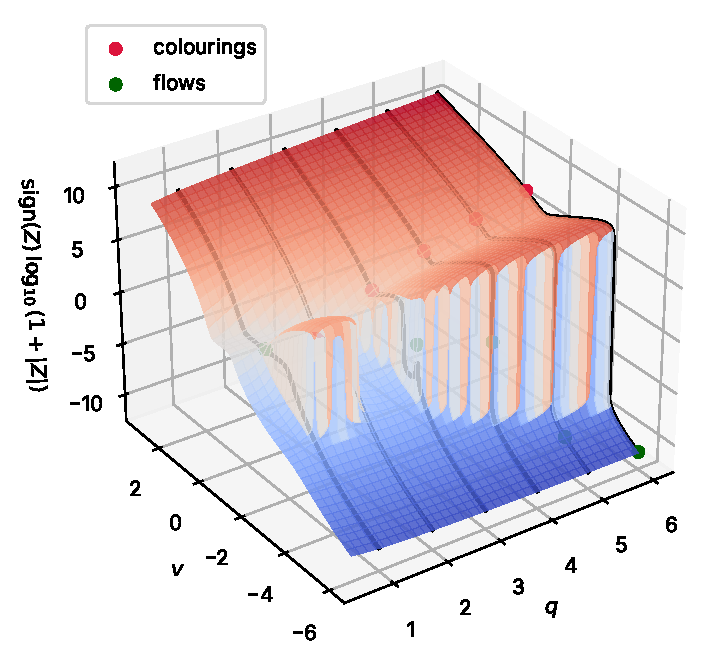
\includegraphics[width=0.78\textwidth]{figures/fig_tutte.pdf}
\caption{The random-cluster partition function $Z(G;q,v)$ of the Petersen graph
over the $(q,v)$-plane, as $\operatorname{sign}(Z)\log_{10}(1+|Z|)$, computed from
the $2^{15}$ edge subsets. Theorem~\ref{thm:tutte} evaluates it along the lines
$q=1,2,3,\dots$ drawn on the surface, which are the hyperbolas $H_q$ of the
Tutte plane; the marked points are the proper $q$-colourings ($v=-1$) and the
nowhere-zero flows ($v=-q$).}
\label{fig:tutte}
\end{figure}

\begin{remark}\label{rem:tutte}
Evaluating the Tutte polynomial is $\#$P-hard at every point of the plane
except on the hyperbola $H_1$ and at eight special points \cite{JVW90}; the
points of $H_q$ for positive integers $q$ include the chromatic and flow
polynomials at $q$, the Ising model ($q=2$) and the Potts models. On
bounded-degree graphs Theorem~\ref{thm:tutte} evaluates all of them in time
$2^{o(n)}$. The theorem does not evaluate $T$ off these hyperbolas: the number
of acyclic orientations $T(G;2,0)$, which lies on $H_{-1}$, the number of
forests $T(G;2,1)$ on $H_0$, and the reliability polynomial on $H_1$, trivial,
are not covered, and neither is the chromatic polynomial as a polynomial in $q$,
which would need the values at $n+1$ integers $q$ while the constant in the
exponent grows with $q$.
\end{remark}

\subsection{Linear codes with sparse parity checks}\label{ssec:codes}
A binary linear code of length $n$ given by a parity-check matrix
$H\in\Ftwo^{m\times n}$ is $\mathcal C=\{x\in\Ftwo^n:Hx=0\}$. Its weight
enumerator is the sequence $A_i=\#\{x\in\mathcal C:\operatorname{wt}(x)=i\}$,
$0\le i\le n$, where $\operatorname{wt}$ is the Hamming weight, and its minimum
distance is $d(\mathcal C)=\min\{i\ge1:A_i>0\}$. For a received word
$y\in\Ftwo^n$ the distance distribution of $y$ is
$A_i(y)=\#\{x\in\mathcal C:\operatorname{wt}(x+y)=i\}$, the weight enumerator of
the coset $y+\mathcal C$; a codeword at distance $\min\{i:A_i(y)>0\}$ from $y$ is a
maximum-likelihood decoding of $y$ on the binary symmetric channel. The codes
whose parity-check matrix has rows of bounded weight are the low-density
parity-check codes of Gallager \cite{Gal62}.

\begin{theorem}[Sparse parity checks]\label{thm:codes}
Fix $k,c\ge1$. Let $\mathcal C\subseteq\Ftwo^n$ be given by a parity-check matrix
with $m\le cn$ rows, each of weight at most $k$.
\begin{enumerate}[label=\textup{(\roman*)},leftmargin=2.2em]
\item\label{it:wenum} The weight enumerator $(A_i)_{0\le i\le n}$, and hence
$d(\mathcal C)$ and the number of minimum-weight codewords, are computed
deterministically in time $\poly(n)2^{O_{k,c}(\rhon(n))}$.
\item\label{it:coset} For every $y\in\Ftwo^n$ the distance distribution
$(A_i(y))_i$ is computed in the same time, and a codeword nearest to $y$ is
found in $2n+1$ times that time.
\item\label{it:qary} For a code over a finite field $\mathbb F_Q$, or over any
alphabet of fixed size $Q$ with the checks given as tables on $[Q]^{k}$, given by
$m\le cn$ checks each involving at most $k$ coordinates, the Hamming weight
enumerator and the distance distribution of every received word are computed
in time $\poly(n)2^{O_{Q,k,c}(\rhon(n))}$; so is the complete weight enumerator,
the number of codewords with $i_s$ coordinates equal to $s$ for each symbol
$s$, in time $\poly(n^{Q})2^{O_{Q,k,c}(\rhon(n))}$.
\end{enumerate}
\end{theorem}

\begin{proof}
\ref{it:wenum} Boolean variables $x_1,\dots,x_n$ and $\A=\A_{n+1}$. For each row
$h$ of $H$ take the multilinear extension of the indicator, on the scope
$\operatorname{supp}(h)$ of size at most $k$, that $\sum_{v\in\operatorname{supp}(h)}x_v$
is even; its coefficients are integers of absolute value at most $2^{k}$. For
each coordinate take $1+(W-1)Y_v$. There are at most $(c+1)n$ factors of scope at
most $k$, and the sum is $\sum_{x\in\mathcal C}W^{\operatorname{wt}(x)}=\sum_iA_iW^{i}$,
with no truncation. Theorem~\ref{thm:weighted} and Lemma~\ref{lem:bits} with
$N=n+1$, $L=k$ give the time; $d(\mathcal C)$ and $A_{d}$ are read off.

\ref{it:coset} Replace the coordinate factor by the multilinear extension of
$W^{[x_v\ne y_v]}$, which is $1+(W-1)Y_v$ if $y_v=0$ and $W+(1-W)Y_v$ if $y_v=1$;
the sum is $\sum_{x\in\mathcal C}W^{\operatorname{wt}(x+y)}=\sum_iA_i(y)W^{i}$. For
the nearest codeword let $i_0=\min\{i:A_i(y)>0\}$ and fix the coordinates one at
a time: fixing $x_1=\epsilon$ replaces every row containing coordinate $1$ by
the indicator that the remaining coordinates have parity $\epsilon h_1$, a
factor of smaller scope, and leaves the system sparse; compute the two distance
distributions, keep a value $\epsilon$ for which the coefficient of
$W^{i_0}$ is positive, and continue with the next coordinate. After $n$ steps the
assignment is a codeword at distance $i_0$ from $y$, and $2n+1$ distributions
have been computed.

\ref{it:qary} Apply Theorem~\ref{thm:domain} with $D=Q$: the variables take
values in the alphabet, each check is a table on at most $k$ coordinates, and
the coordinate factor has the table $s\mapsto W^{[s\ne0]}$, or
$s\mapsto W^{[s\ne y_v]}$ for the distance to $y$, in $\A_{n+1}$; for the
complete weight enumerator the table is $s\mapsto W_s$ in
$\A_{n+1,\dots,n+1}$ with one generator per symbol, of dimension $(n+1)^{Q}$.
\end{proof}

\begin{remark}
Computing the minimum distance of a binary linear code is NP-hard
\cite{Var97}, and so is maximum-likelihood decoding \cite{BMT78}; both are
posed with the code given by a generator or a parity-check matrix of
unrestricted density. For the low-density codes of Gallager, with $m\le n$ rows
of bounded weight, Theorem~\ref{thm:codes} gives the exact minimum distance, the
complete weight enumerator and exact maximum-likelihood decoding of every
received word in deterministic time $2^{o(n)}$, where the previously known
exact methods are exponential in the dimension or the redundancy of the code.
No bound on the column weights is needed, by Lemma~\ref{lem:frequent}.
\end{remark}

\subsection{Bounded-degree hypergraphs}\label{ssec:hypergraphs}
A hypergraph $\mathcal H=(V,\mathcal E)$ has vertex set $V$, $|V|=n$, and a
multiset $\mathcal E$ of edges $e\subseteq V$. A matching is a set of pairwise
disjoint edges, a perfect matching or exact cover is a matching whose union is
$V$, a transversal is a set of vertices meeting every edge, an independent set is
a set of vertices containing no edge, and a strong independent set is a set of
vertices no two of which lie in a common edge. A $q$-colouring of $V$ is proper
if no edge of size at least two is monochromatic.

\begin{theorem}[Hypergraphs]\label{thm:hypergraphs}
Fix $k,\Delta,c\ge1$ and $q\ge2$, and let $\mathcal H$ have $n$ vertices and
edges of size at most $k$.
\begin{enumerate}[label=\textup{(\roman*)},leftmargin=2.2em]
\item\label{it:hmatch} If every vertex lies in at most $\Delta$ edges and the
edges have integer weights in $[0,\Omega]$: the number of matchings of each
weight and the number of exact covers of each weight, hence the maximum weight
of a packing and the number of exact covers, in time
$\poly(n,\Omega)2^{O_{k,\Delta}(\rhon(n))}$.
\item\label{it:hindep} If $|\mathcal E|\le cn$ and the vertices have integer
weights in $[0,\Omega]$: the number of transversals, of independent sets and of
strong independent sets of each weight, in time
$\poly(n,\Omega)2^{O_{k,c}(\rhon(n))}$.
\item\label{it:hcol} If $|\mathcal E|\le cn$: the number of proper
$q$-colourings, and the number of $q$-colourings with exactly $j$ monochromatic
edges for every $j$, in time $\poly(n)2^{O_{q,k,c}(\rhon(n))}$.
\end{enumerate}
\end{theorem}

\begin{proof}
\ref{it:hmatch} A vertex in no edge lies in no exact cover and in every matching
trivially; delete such vertices, so that $n\le k|\mathcal E|$, and if
$|\mathcal E|<20$ list the subsets. Boolean variables $y_e$, $e\in\mathcal E$;
for each vertex $v$ the multilinear extension on the scope
$\{e:v\in e\}$, of size at most $\Delta$, of the indicator that at most one
(for matchings) or exactly one (for exact covers) incident edge is chosen; for
each edge $1+(W^{\omega_e}-1)Y_e$. There are $n+|\mathcal E|\le(k+1)|\mathcal E|$
factors of scope at most $\Delta$, the sum is
$\sum_M W^{\omega(M)}$ over the matchings, or over the exact covers, in $\A_N$
with $N=1+\sum_e\omega_e$, and Theorem~\ref{thm:weighted} on $|\mathcal E|\le\Delta n$
variables with the constants $\Delta$ and $k+1$, with Lemma~\ref{lem:bits},
$L=\Delta$, gives the bound; $\rhon(|\mathcal E|)=O_\Delta(\rhon(n))$.

\ref{it:hindep} Boolean variables $x_v$; for each edge $e$ the multilinear
extension, on the scope $e$, of the indicator that some $x_v$, $v\in e$, is $1$
(transversals), that not all are $1$ (independent sets), or that at most one
is $1$ (strong independent sets); for each vertex $1+(W^{\omega_v}-1)Y_v$. At most
$(c+1)n$ factors of scope at most $k$; Theorem~\ref{thm:weighted} and
Lemma~\ref{lem:bits} with $L=k$.

\ref{it:hcol} Theorem~\ref{thm:domainprofile} with $D=q$ and, for each edge of
size at least two, the constraint that it is monochromatic, of weight $1$: the
coefficient $p_j$ counts the colourings with $j$ monochromatic edges and $p_0$
the proper ones.
\end{proof}

\subsection{Circuits of linear size}\label{ssec:circuits}
A Boolean circuit with $n$ inputs is a sequence of gates $g_1,\dots,g_s$, each
computing a function of at most $k$ earlier gates or inputs given by its truth
table, with $t$ of the gates designated as outputs. Its size is $s$.

\begin{theorem}[Linear-size circuits of bounded fan-in]\label{thm:circuits}
Fix $k,c\ge1$. Let $C$ be a circuit with $n\ge20$ inputs, $s\le cn$ gates of
fan-in at most $k$, and outputs $o_1,\dots,o_t$ with integer weights
$\omega_1,\dots,\omega_t\in[0,\Omega]$. The numbers
\[
  N_{i,j}=\#\Bigl\{x\in\{0,1\}^n:\ \operatorname{wt}(x)=i,\ \sum_{l=1}^{t}\omega_l\,o_l(x)=j\Bigr\}
\]
are computed deterministically, for all $(i,j)$, in time
$\poly(n,\Omega)2^{O_{k,c}(\rhon(n))}$. In particular the number of inputs
accepted by a single-output circuit, and the maximum over the inputs of a
weighted sum of its output bits with the number of inputs attaining it, are
computed in that time.
\end{theorem}

\begin{proof}
Take the $n+s$ Boolean variables $x_1,\dots,x_n,g_1,\dots,g_s$ and
$\A=\A_{n+1,\,1+\sum_l\omega_l}$ with generators $U$ and $W$. For each gate $g$
take the multilinear extension, on the scope consisting of $g$ and its at most
$k$ arguments, of the indicator that $g$ equals the value of its function at the
arguments; for each input $1+(U-1)Y_{x_v}$; for each output $o_l$ the factor
$1+(W^{\omega_l}-1)Y_{o_l}$. There are $s+n+t\le(2c+1)n\le(2c+1)(n+s)$ factors of
scope at most $k+1$, with coefficients of absolute value at most $2^{k+1}$. For
each input $x$ exactly one assignment of the gate variables makes every gate
factor $1$, the one in which each $g$ carries its value at $x$, and every other
assignment makes some gate factor $0$; so the sum over the cube is
$\sum_xU^{\operatorname{wt}(x)}W^{\sum_l\omega_lo_l(x)}=\sum_{i,j}N_{i,j}U^{i}W^{j}$,
with nothing truncated. Theorem~\ref{thm:weighted} on $n+s\le(c+1)n$ variables
with the constants $k+1$ and $2c+1$, and Lemma~\ref{lem:bits} with $L=k+1$,
give the time, since $\rhon(n+s)\le\rhon((c+1)n)=O_c(\rhon(n))$.
\end{proof}

\begin{remark}
The count of the accepted inputs of a circuit with $s$ gates is, through the
Tseitin encoding used in the proof, the count of the satisfying assignments of a
$(k+1)$-CNF formula with $n+s$ variables, so for every $s$ it is contained in
\oai{}'s Theorem~1.1 with the exponent $o(n+s)$; their Corollary~1.4 draws a
circuit lower bound from exactly this fact. Theorem~\ref{thm:circuits} adds the
Hamming weight of the input and the weighted output profile for the sparse
case, which turns any objective computable by a linear-size circuit of bounded
fan-in on $n$ Boolean variables into one that is maximised exactly in time
$2^{o(n)}$, together with the number of maximisers. Theorems \ref{thm:profile},
\ref{thm:edges} and \ref{thm:codes} are instances, since their constraints are
computed by such circuits; the direct encodings given there avoid the gate
variables and have smaller constants.
\end{remark}

\subsection{Integer programs with sparse rows}\label{ssec:ip}
A $0$-$1$ integer program asks for a vector $x\in\{0,1\}^n$ satisfying a system
of linear inequalities and maximising a linear objective. Its rows need not
be clauses, cuts or parity checks: a row is an arbitrary linear form with
integer coefficients, compared with an integer by $\le$, $=$ or $\ge$. When
every row involves at most $k$ variables and there are $O(n)$ of them, each row
is a local constraint, and Theorem~\ref{thm:linear} adds a fixed number of
dense rows and the objective as linear statistics.

\begin{theorem}[Sparse integer programs]\label{thm:ip}
Fix integers $k,c\ge1$ and $s\ge0$. Consider $n\ge20$ variables, $m\le cn$
sparse rows
\[
  \sum_{v\in I_f}a_{f,v}x_v\ \bowtie_f\ b_f,\qquad |I_f|\le k,\quad
  {\bowtie_f}\in\{\le,=,\ge\},\quad a_{f,v},b_f\in\Z,
\]
with coefficients of arbitrary size, a cost vector $\gamma$ and dense rows
$\alpha^{(1)},\dots,\alpha^{(s)}$ in $\{-\Omega,\dots,\Omega\}^n$, $\Omega\ge1$,
and let $P\subseteq\{0,1\}^n$ be the set of vectors satisfying the sparse rows.
\begin{enumerate}[label=\textup{(\roman*)},leftmargin=2.2em]
\item\label{it:ip01} The numbers
\[
  p(j_0,\dots,j_s)=\#\bigl\{x\in P:\ \gamma\cdot x=j_0,\ \alpha^{(i)}\cdot x=j_i\ (1\le i\le s)\bigr\}
\]
are computed for all tuples in time
$\poly\bigl(\ell,(1+2n\Omega)^{s+2}\bigr)\,2^{O_{k,c,s}(\rhon(n))}$, where $\ell$
is the bit length of the input. Hence the largest and the smallest value of
$\gamma\cdot x$ over the $x\in P$ with $\alpha^{(i)}\cdot x\bowtie_i\beta_i$ for
prescribed relations $\bowtie_i$ and integers $\beta_i$, and the number of
vectors attaining each, are computed within the same time.
\item\label{it:ipD} For a fixed $D\ge1$ the same holds for vectors
$x\in\{0,1,\dots,D\}^n$, with time
$\poly\bigl(\ell,(1+4Dn\Omega)^{s+2}\bigr)\,2^{O_{D,k,c,s}(\rhon(n))}$.
\end{enumerate}
\end{theorem}

\begin{proof}
\ref{it:ip01} For each sparse row let $\phi_f:\{0,1\}^{I_f}\to\{0,1\}$ be the
indicator that the row holds, and let $\Phi_f$ be its multilinear extension
\eqref{eq:multilinear}. The table of $\phi_f$ has at most $2^k$ entries, each
found by one evaluation of the row, at a cost of $\poly(\ell)$ bit operations;
the coefficients of $\Phi_f$ are integers of absolute value at most $2^k$. So
$(\Phi_f)$ is a factor system with at most $cn$ factors of scope at most $k$
and values in $\Q$, and its product at $x\in\{0,1\}^n$ is the indicator of $P$.
To bring the statistics to nonnegative weights, put
$\omega^{(0)}_v=\gamma_v+\Omega$, $\omega^{(i)}_v=\alpha^{(i)}_v+\Omega$ for
$1\le i\le s$, and $\omega^{(s+1)}_v=1$, all in $[0,2\Omega]$. For every $x$,
\[
  \gamma\cdot x=\omega^{(0)}\cdot x-\Omega\,|x|,\qquad
  \alpha^{(i)}\cdot x=\omega^{(i)}\cdot x-\Omega\,|x|,\qquad |x|=\omega^{(s+1)}\cdot x .
\]
Theorem~\ref{thm:linear}\ref{it:lineq} with $N_0=1$, the $s+2$ weight vectors
$\omega^{(0)},\dots,\omega^{(s+1)}$ and the weight bound $2\Omega$ computes the
numbers $r(j'_0,\dots,j'_{s+1})$ of $x\in P$ with $\omega^{(i)}\cdot x=j'_i$ for
all $i$, in time $\poly(n,(1+2n\Omega)^{s+2})2^{O_{k,c,s}(\rhon(n))}$, to which
the cost $cn2^k\poly(\ell)$ of the tables is added. Then
\[
  p(j_0,\dots,j_s)=\sum_{t=0}^{n}r\bigl(j_0+\Omega t,\ j_1+\Omega t,\dots,\ j_s+\Omega t,\ t\bigr),
\]
because a vector with $|x|=t$ has $\omega^{(i)}\cdot x=\alpha^{(i)}\cdot x+\Omega t$.
The optimum over the $x\in P$ with $\alpha^{(i)}\cdot x\bowtie_i\beta_i$ is the
largest, or smallest, $j_0$ for which $\sum p(j_0,j_1,\dots,j_s)>0$, the sum
taken over the tuples with $j_i\bowtie_i\beta_i$, and that sum counts the
optimal vectors.

\ref{it:ipD} Let $T=\lceil\log_2(D+1)\rceil$ and replace each $x_v$ by $T$
Boolean variables $x_{v,0},\dots,x_{v,T-1}$ with $x_v=\sum_t2^tx_{v,t}$. A sparse
row becomes a sparse row in the new variables, with the coefficients
$2^ta_{f,v}$ and at most $kT$ variables; add for each $v$ the row
$\sum_t2^tx_{v,t}\le D$, which involves $T$ variables. The cost and the dense
rows become vectors with entries $2^t\gamma_v$ and $2^t\alpha^{(i)}_v$, of
absolute value at most $2^T\Omega\le2(D+1)\Omega\le4D\Omega$. The new program
has $n'=Tn$ variables and at most $(c+1)n\le(c+1)n'$ sparse rows of at most $kT$
variables, and its feasible vectors correspond bijectively to the vectors of
$\{0,\dots,D\}^n$ satisfying the original sparse rows, with the same values of
$\gamma\cdot x$ and $\alpha^{(i)}\cdot x$. Part \ref{it:ip01} applies, with
$\rhon(Tn)\le4T\rhon(n)$ for $n\ge T$.
\end{proof}

The theorem places no bound on the coefficients of the sparse rows, only on
their number of variables; the polynomial bound $\Omega$ is needed only for the
objective and the dense rows, which enter through the exponents of the
generators. Three classical problems that are NP-hard in the strong sense fall
under it.

\begin{corollary}\label{cor:ip}
Fix $k,c,s\ge1$. Each of the following is computed deterministically in time
$\poly(\ell,\Omega^{s+2})\,2^{O(\rhon(n))}$, where $\ell$ is the length of the
input, together with the number of optimal solutions, the implied constant
depending on $k,c,s$.
\begin{enumerate}[label=\textup{(\alph*)},leftmargin=2.2em]
\item\label{it:exactcover} For $n$ sets over a universe of at most $cn$
elements, each element lying in at most $k$ of the sets, with costs in
$[0,\Omega]$: the least cost of an exact cover, of a set cover and the largest
cost of a set packing. Exact cover by $3$-sets is NP-complete already when
every element lies in exactly three sets \cite{Gon85}.
\item\label{it:poknap} For $n$ items with values and $s$ weight vectors in
$[0,\Omega]$, capacities $B_1,\dots,B_s$ and a partial order given by at most
$cn$ relations $u\prec v$: the largest value of a set of items within the
capacities that contains, with each item, every item below it. For $s=1$ this
is the partially ordered knapsack problem, which is NP-complete in the strong
sense \cite{JN83}.
\item\label{it:exactsat} For a system of at most $cn$ linear equations
$\sum_{v\in I_f}a_{f,v}x_v=b_f$ with integer coefficients, $|I_f|\le k$, and a
cost vector in $[-\Omega,\Omega]^n$: the number of its $0$-$1$ solutions of
each cost, and the least and largest cost; in particular the number of
solutions of a $1$-in-$k$-SAT instance with at most $cn$ clauses, and its
solutions with the fewest true variables.
\end{enumerate}
\end{corollary}

\begin{proof}
\ref{it:exactcover} Take a variable for each set and, for each element, the
row $\sum_{S\ni e}x_S=1$, $\ge1$ or $\le1$; each row involves at most $k$
variables, and there are at most $cn$ rows. The cost is $\gamma$, with $s=0$.
\ref{it:poknap} Take a variable for each item, the row $x_v-x_u\le0$, which
says that $x_v=1$ forces $x_u=1$, for each relation $u\prec v$, and the weight
vectors as dense rows with $\beta_i=B_i$ and $\bowtie_i$ the relation $\le$;
the downward closure of the chosen set under the given relations is
equivalent to its closure under the order they generate. \ref{it:exactsat}
The equations are the sparse rows; for $1$-in-$k$-SAT a clause on the
literals $\ell_1,\dots,\ell_k$ is the equation $\sum_i\ell_i=1$, where a
negated literal $1-x_v$ moves the constant $1$ to the right side. All three
are Theorem~\ref{thm:ip}\ref{it:ip01}.
\end{proof}

\subsection{Growing density}\label{ssec:density}
Every statement so far fixes the ratio $c$ of factors to variables. The
parameters of Lemma~\ref{lem:params} do not depend on the degree ratio
$\kappa$, and the exponent of Theorem~\ref{thm:bounded-occ} is linear in it.
When $\kappa$ grows with $n$ it pays to let the parameters follow it: fewer
groups, and so a smaller $Q/R$ in the Taylor count, in exchange for a larger
share of the cost spent on one group. With the entropy bound of
Lemma~\ref{lem:entropy} in place of \eqref{eq:logCq}, this extends the
subexponential regime to every ratio $\kappa=o(\sqrt{\log n/\log\log n})$.

Throughout, $\lambda=\lceil\log n\rceil$, $\nu=\lceil\log\lambda\rceil$, and
\[
  g(x)=x\,\bigl(\log(1/x)\bigr)^{3/2}\qquad(0<x<1),
\]
which is increasing on $(0,2^{-3}]$ and tends to $0$ with $x$.

\begin{theorem}[Bounded occurrences at a growing degree ratio]\label{thm:explicit}
There is an absolute constant $\lambda_0$ with the following property. Let $\A$
be a commutative $\Q$-algebra, and let a factor system on $n$ variables with
$\lambda\ge\lambda_0$ have largest scope $w\le\lambda^2$, largest occurrence
number $b\le\lambda^2-1$ and total degree $d\le an$, where $a\ge1$ is a
real number with
\[
  \theta:=a\sqrt{\nu/\lambda}\le2^{-15}.
\]
Then $Z$ in \eqref{eq:Z} is computed deterministically with at most
\begin{equation}\label{eq:explicit}
  |\F|\,\poly(n)\,2^{\,790\,n\,g(\theta)}
\end{equation}
operations in $\A$, evaluations of factors at inputs in $\Q[z]/(z^{J})$ with
$J\le n$, and bit operations on rational numbers, using polynomially many
elements of $\A$ and polynomially many bits of storage in addition to the
factors' own. The polynomial is absolute.
\end{theorem}

\begin{proof}
Adjoin the constant-one factors of Section~\ref{sec:design}, so that
\eqref{eq:nMb} holds with $b\le\lambda^2$ and $d$ unchanged. Replacing $a$ by
$\max(1,d/n)$, which is rational, computed from the input and not larger than $a$,
decreases $\theta$ and, as $g$ is increasing, the bound \eqref{eq:explicit}; so we
may assume $a=\max(1,d/n)$. Put
$L=\log(1/\theta)\ge15$ and choose
\[
  t=\lfloor L\rfloor,\quad r=2^{t},\quad Q=\Bigl\lfloor\frac{\lambda}{128t}\Bigr\rfloor,\quad
  R=32+\bigl\lceil16\sqrt{Q\nu}\,\bigr\rceil,\quad \tau=\frac1{r\lambda},\quad D=r^{2Q}.
\]
Thus $t$ is the largest integer with $4^ta^2\nu\le\lambda$, and $1/(2\theta)<r\le1/\theta$.
Since $a\ge1$ and $\lambda\le2^{\nu}$, $L\le\frac12\log(\lambda/\nu)\le\nu/2$, so
$t\le\nu/2$ and $r^2\le2^{\nu}\le2\lambda$.

We check the hypotheses of Lemma~\ref{lem:complete}. First, $\lambda\ge256t$, so
$Q\ge\lambda/(256t)$, and $\log D=2Qt\le\lambda/64$. Since $Q\nu\ge1$,
$R\le33+16\sqrt{Q\nu}\le49\sqrt{Q\nu}$, hence
\begin{equation}\label{eq:RQexplicit}
  \frac RQ\le49\sqrt{\frac\nu Q}\le784\sqrt{\frac{t\nu}{\lambda}}
  \le784\,\frac{\nu}{\sqrt{2\lambda}} ,
\end{equation}
which is at most $1/6$ once $\lambda\ge(6\cdot784)^2\nu^2/2$; so $R\ge32$, $6R\le Q$
and $R<Q$ for $\lambda\ge\lambda_0$. The balance conditions \eqref{eq:balance}
hold: $2(b+w)D^2\le4\lambda^2\,2^{\lambda/32}\le2^{\lambda-1}<n\le M$ and
$2Qr^2\le(\lambda/64t)\cdot2\lambda<n$ for $\lambda\ge\lambda_0$. For the interval
take $\mu=Q(r-1)/(2r)$, $A_0=\lfloor\mu-(R-1)/2\rfloor$ and
$\mathcal J=\{A_0,\dots,A_0+R-1\}$ as in the proof of Lemma~\ref{lem:params}; since
$R\le Q/6$ it lies in $\{0,\dots,Q\}$, and since $R\ge32$ it contains every integer
within $R/4$ of $\mu$. Hoeffding's inequality \eqref{eq:hoeffding} with $s=R/4$
and $R^2\ge256Q\nu$ gives
\[
  \Pr\Bigl[\Bin\Bigl(Q,\tfrac{r-1}{2r}\Bigr)\notin\mathcal J\Bigr]\le2e^{-R^2/(8Q)}
  \le2e^{-32\nu}\le2^{-4\nu}\le\frac1{r^2\,b\,\lambda}=\frac{\tau}{rb},
\]
because $r^2\le2^{\nu}$, $b\le\lambda^2\le2^{2\nu}$ and $\lambda\le2^{\nu}$. This is
\eqref{eq:tailreq}, and $0<\tau\le1/2$. Lemma~\ref{lem:complete} constructs the
design in polynomial time.

Now the costs of Proposition~\ref{prop:routine}. By \eqref{eq:degbound} with
$d\le an$, $q=\lfloor dR/Q\rfloor\le\chi n$ with $\chi=aR/Q$. Since
$\sqrt{\nu/\lambda}=\theta/a\le\theta$ and $t\le L$, \eqref{eq:RQexplicit} gives
\[
  \chi\le784\,a\sqrt{\frac{t\nu}{\lambda}}\le784\,\theta\sqrt L=:\bar\chi ,
\]
and $\bar\chi\le784\cdot2^{-15}\sqrt{15}<\frac1{10}$ because $x\sqrt{\log(1/x)}$
increases on $(0,2^{-15}]$. In particular $q\le n/2$ and $J=q+1\le n$.
Lemma~\ref{lem:entropy} and the monotonicity of $x\log(2en/x)$ in $x\le n$ give
\[
  \log C_q\le\bar\chi n\log\frac{2e}{\bar\chi}
  =784\,\theta\sqrt L\,n\Bigl(L+\log\frac{2e}{784\sqrt L}\Bigr)\le784\,n\,\theta L^{3/2}
  =784\,n\,g(\theta).
\]
The measurement count contributes
$2\tau n\log(2D+1)\le\frac{2n}{r\lambda}\bigl(\frac\lambda{64}+2\bigr)\le\frac nr$
and one group $\frac{2n}r$, together $\frac{3n}{r}<6n\theta\le6\,n\,g(\theta)$.
The logarithm of \eqref{eq:routinecost} is therefore at most
$\log(2Qr)+790\,n\,g(\theta)$. Each vector costs at most $|\F|$ factor evaluations
and a number of further operations polynomial in $n$, $|\F|$, $D$, $Q$, $R$, $J$,
$r$ and $M\le\lambda^2 n$, all of which are bounded by powers of $n$ and $|\F|$
since $D\le2^{\lambda/64}\le2n^{1/64}$. The storage bound is that of
Proposition~\ref{prop:routine}.

The parameters are computed from $n$ and $d$ with integer square roots and
exact rational comparisons, in $\poly(\log n,\log d)$ bit operations,
and the conditions of Lemma~\ref{lem:complete} are checked exactly as in the proof
of Lemma~\ref{lem:params}; the estimates above show that every check passes.
\end{proof}

For a fixed ratio $a$ one has $\theta=a\sqrt{\nu/\lambda}$ and $\log(1/\theta)\le\nu/2$,
so $g(\theta)\le a\nu^2/(2\sqrt{2\lambda})$, and \eqref{eq:explicit} is the bound of
Theorem~\ref{thm:bounded-occ} with $\beta=2$ up to the constant. The gain is in the
dependence on $a$: the exponent of Theorem~\ref{thm:bounded-occ} is
$a\,n\nu^2/\sqrt\lambda$, which is $o(n)$ only for $a=o(\sqrt\lambda/\nu^2)$, while
$n\,g(\theta)$ is $o(n)$ for every $a=o(\sqrt{\lambda/\nu})$. Two changes produce the
gain. The entropy bound \eqref{eq:Cqentropy} charges the Taylor count
$\log C_q\approx q\log(n/q)$, whereas \eqref{eq:logCq} charges $q\log(Q/R)$, larger by
the factor $\log(Q/R)/\log(Q/(aR))$, which grows with $a$. And the number of groups
$r=2^{\lfloor\log(1/\theta)\rfloor}$ shrinks as $a$ grows, which makes $Q$ larger and
$R/Q$ smaller at the price of the cost $3n/r$ of the groups, balanced against the
Taylor count.

\begin{theorem}[Growing density]\label{thm:density}
There are absolute constants $n_1$ and $\theta_1>0$ with the following property.
Let $n\ge n_1$, let $k\ge1$ be an integer and $c\ge1$ a real number with
\[
  \theta_n:=ck\sqrt{\frac{\log\log n}{\log n}}\le\theta_1,
\]
and let a factor system on $n$ variables have at most $cn$ factors, each of scope
at most $k$, with values in a commutative $\Q$-algebra $\A$. Then $Z$ in
\eqref{eq:Z} is computed deterministically with at most
\[
  \poly(n)\,2^{\,4800\,n\,g(\theta_n)}\ \le\ \poly(n)\,2^{\,1700\,ck\,\rhon(n)}
\]
operations in $\A$, evaluations of the factors at inputs in $\Q[z]/(z^{J})$,
$J\le n$, and bit operations on rationals, in polynomial space; the polynomial is
absolute. In particular the bound is $2^{o(n)}$ whenever
$ck=o\bigl(\sqrt{\log n/\log\log n}\bigr)$. If the coefficients of the factors are
polynomials in the generators of $\A=\A_N$ or $\A_{N_1,\dots,N_s}$ with integer
coefficients of at most $L$ bits, the bound holds for bit operations after
multiplication by a polynomial in $n$, $N$ and $L$.
\end{theorem}

\begin{proof}
Put $\theta_1=2^{-18}$ and $\varepsilon_n=\sqrt{\log\log n/\log n}$, so that
$\theta_n=ck\,\varepsilon_n\ge\varepsilon_n$. Let $n_1$ be so large that for
$n\ge n_1$ one has $\lambda-1\ge\lambda_0$, the absolute constant of
Theorem~\ref{thm:explicit}, and $\theta_1\sqrt{\log n/\log\log n}\le\lambda/2$, so
that $ck\le\lambda/2$. Apply Lemma~\ref{lem:frequent}: fewer than $2^{n/\lambda}$
assignments $y$, each leaving a system on $n'\ge n-n/\lambda\ge n/2$ variables with
$\lambda'=\lceil\log n'\rceil\in\{\lambda-1,\lambda\}$, $\nu'\le\nu$, scopes at most
$k\le\lambda'^2$, occurrence numbers at most $ck\lambda\le\lambda^2/2\le\lambda'^2-1$,
and total degree at most $kcn\le2ck\,n'$. Theorem~\ref{thm:explicit} applies with
$a=2ck$ and
\[
  \theta'=2ck\sqrt{\nu'/\lambda'}\le2ck\sqrt{2\nu/\lambda}\le6\,ck\,\varepsilon_n=6\theta_n\le2^{-15},
\]
where $\nu\le\log\log n+2\le3\log\log n$ and $\lambda\ge\log n$ were used for $n\ge20$.
As $g$ is increasing on $(0,2^{-3}]$,
$g(\theta')\le g(6\theta_n)\le6\theta_n\log^{3/2}(1/\theta_n)=6\,g(\theta_n)$.
Each $Z_y$ costs at most $cn\,\poly(n)\,2^{4740\,n\,g(\theta_n)}$ operations, and
$cn\le n^2$. The branching adds the factor $2^{n/\lambda}\le2^{n\varepsilon_n}\le2^{n\,g(\theta_n)}$,
since $1/\lambda\le1/\log n\le\varepsilon_n\le\theta_n$ and $\log(1/\theta_n)\ge18$. The total is
at most $\poly(n)2^{4741\,n\,g(\theta_n)}$, which gives the first bound. For the second,
$\log(1/\theta_n)\le\log(1/\varepsilon_n)\le\frac12\log\log n$, so
$g(\theta_n)\le ck\,\varepsilon_n(\log\log n)^{3/2}/2^{3/2}=ck\,\rhon(n)/(2^{3/2}n)$,
and $4800/2^{3/2}<1700$. If $ck=o(\sqrt{\log n/\log\log n})$ then $\theta_n\to0$ and
$g(\theta_n)\to0$. The space bound and $J\le n'\le n$ come from
Theorem~\ref{thm:explicit}, and the bit complexity is Lemma~\ref{lem:bits}: its
proof uses of the parameters only $Q,\lambda=O(\log n)$, $R<Q$ and $D\le2^{\lambda}$,
which hold here, and its polynomial depends on $|\F|\le n^2$ and $k\le\lambda^2$ only
through powers of $n$.
\end{proof}

The corollaries of Sections \ref{sec:applications} and \ref{sec:more} that are
proved by one application of Theorem~\ref{thm:weighted} to a factor system whose
number of factors is bounded by the number of constraints or edges of the input,
and whose scopes are bounded, therefore extend to inputs of growing density. For a
function $d(n)\ge1$ write
\[
  \delta_n=d(n)\sqrt{\frac{\log\log n}{\log n}} ;
\]
the condition $\delta_n\to0$ means $d(n)=o(\sqrt{\log n/\log\log n})$. We record the
two for which the question of the dense case was raised in the introduction.

\begin{corollary}[Cuts and spin systems at growing average degree]\label{cor:density}
Let $d=d(n)\ge1$ satisfy $\delta_n\to0$, and let $G$ be a graph with $n$ vertices and
at most $d(n)\,n$ edges.
\begin{enumerate}[label=(\roman*),leftmargin=2.2em]
\item\label{it:densecut} The cut profile $\bigl(\#\{S\subseteq V:|S|=i,\
e(S,V\setminus S)=j\}\bigr)_{i,j}$, in particular the maximum cut, the maximum
bisection and their numbers of optimal solutions, is computed in time
$\poly(n)\,2^{\,20000\,n\,g(\delta_n)}=2^{o(n)}$.
\item\label{it:denseising} The density of states of an Ising system on $G$
with integer couplings and fields, and that of the $q$-state Potts system on
$G$ for fixed $q$, are computed in time
$\poly(n,E_{\max})\,2^{\,O_q(n\,g(\delta_n))}=\poly(E_{\max})\,2^{o(n)}$.
\end{enumerate}
In particular the maximum cut and the ground-state energy of an Ising system on
a graph of average degree $d(n)$ are found in time $2^{o(n)}$ whenever
$d(n)=o(\sqrt{\log n/\log\log n})$.
\end{corollary}

\begin{proof}
\ref{it:densecut} The factor system of Corollary~\ref{cor:maxcut} has one factor
of scope $2$ per edge and one of scope $1$ per vertex, with values in
$\A_{n+1,\,m+1}$ and coefficients of absolute value at most $2$; so it has at
most $(d(n)+1)n\le2d(n)n$ factors of scope at most $2$. Theorem~\ref{thm:density}
with $k=2$ and $c=2d(n)$ applies once $4\delta_n\le\theta_1$, and gives
$\poly(n)2^{4800\,n\,g(4\delta_n)}$ operations; $g(4\delta_n)\le4g(\delta_n)$, and
Lemma~\ref{lem:bits} with $N=(n+1)(m+1)\le n^3$ and $L=1$ turns the count into the
time bound. The optimum and its multiplicity are read off the profile as in
Corollary~\ref{cor:maxcut}.
\ref{it:denseising} The factor system in the proof of Theorem~\ref{thm:ising}\ref{it:isingmodel}
has one factor of scope $2$ per edge and one of scope $1$ per vertex, with values
in $\A_N$, $N=2E_{\max}+1$, and coefficients of $O(\log E_{\max})$ bits; it has at
most $2d(n)n$ factors, and Theorem~\ref{thm:density} with $k=2$, $c=2d(n)$ and
Lemma~\ref{lem:bits} give the bound as in \ref{it:densecut}. The factor system
in the proof of Theorem~\ref{thm:ising}\ref{it:potts} lives on $n'=qn$ variables
and has $n$ factors of scope $q$ and at most $d(n)n$ of scope $2q$, with
coefficients of $O(q+\log E_{\max})$ bits; so it has at most
$(d(n)+1)n\le(d(n)+1)n'$ factors of scope at most $2q$. Theorem~\ref{thm:density}
on $n'$ variables with $k=2q$ and $c=d(n)+1$ has
$\theta_{n'}\le4q\,d(n)\sqrt{\log\log n'/\log n'}\le4q\,\delta_n$ for large $n$,
because $\log\log x/\log x$ decreases for $x\ge16$; it gives
$\poly(n)2^{4800\,qn\,g(4q\delta_n)}$ operations, and $g(4q\delta_n)\le4q\,g(\delta_n)$.
Lemma~\ref{lem:bits} turns the counts into time bounds, and the ground-state energy
and the partition functions follow as in Theorem~\ref{thm:ising}.
\end{proof}

At $d(n)=\sqrt{\log n}/(\log\log n)^3$, for instance, $\delta_n=(\log\log n)^{-5/2}$
and the exponent in \ref{it:densecut} is $O(n/(\log\log n)^2)$.

The cut function of a graph and that of its complement determine each other, so the
corollary also reaches graphs with $\Theta(n^2)$ edges whose complement is sparse.

\begin{corollary}[Graphs with sparse complements]\label{cor:complement}
Let $d=d(n)\ge1$ satisfy $\delta_n\to0$ and let $\Omega_0\ge1$ be an integer. Let
$H$ be a graph on a vertex set $V$ of size $n$ with at most $d(n)\,n$ edges, and let
$\omega$ be a weighting of the pairs of distinct vertices with $\omega_{uv}=\Omega_0$
for $uv\notin E(H)$ and $\omega_{uv}\in\{0,1,\dots,\Omega_0\}$ for $uv\in E(H)$. Then
the numbers
\[
  p_{i,j}=\#\Bigl\{S\subseteq V:\ |S|=i,\ \sum_{u\in S,\,v\notin S}\omega_{uv}=j\Bigr\}
\]
are computed for all $i,j$ in time $\poly(n,\Omega_0)\,2^{\,O(n\,g(\delta_n))}=\poly(\Omega_0)\,2^{o(n)}$.
In particular, for every graph $G$ on $n$ vertices whose complement has at most
$d(n)\,n$ edges, the cut profile of $G$, the maximum cut, the maximum and the
minimum bisection, and the numbers of optimal solutions, are computed in time
$2^{o(n)}$.
\end{corollary}

\begin{proof}
Put $\eta_{uv}=\Omega_0-\omega_{uv}\in\{0,\dots,\Omega_0\}$ for $uv\in E(H)$. Every pair
$\{u,v\}$ with $u\in S$ and $v\notin S$ carries the weight $\Omega_0$, less
$\eta_{uv}$ when it is an edge of $H$, and there are $|S|(n-|S|)$ such pairs; hence
\begin{equation}\label{eq:complementcut}
  \sum_{u\in S,\,v\notin S}\omega_{uv}=\Omega_0\,|S|\,(n-|S|)-\mathrm{cut}_\eta(S),
\end{equation}
where $\mathrm{cut}_\eta(S)$ is the total $\eta$-weight of the edges of $H$ between $S$
and $V\setminus S$. Corollary~\ref{cor:maxcut}, with Theorem~\ref{thm:density} in place
of Theorem~\ref{thm:weighted} as in the proof of Corollary~\ref{cor:density}\ref{it:densecut},
computes the numbers $q_{i,j}$ of sets $S$ of size $i$ with $\mathrm{cut}_\eta(S)=j$ in
the stated time; the algebra is $\A_{n+1,\,\Omega_0m+1}$ with $m=|E(H)|$, of dimension
polynomial in $n$ and $\Omega_0$. By \eqref{eq:complementcut},
$p_{i,j}=q_{i,\,\Omega_0i(n-i)-j}$, read as $0$ when the index is negative or exceeds
$\Omega_0 m$. For a graph $G$ take $H$ its complement, $\Omega_0=1$ and $\omega=0$ on
$E(H)$; then $\omega$ is the indicator of $E(G)$, and the maximum cut and the bisections
are read off the numbers $p_{i,j}$.
\end{proof}

Corollary~\ref{cor:complement} rests on the fact that the cut of the complete graph
depends on $|S|$ alone. More generally, the cut of a graph whose adjacency is a
fixed quadratic expression in a few vertex weights depends only on the values of
those weights on $S$, and these values are linear statistics in the sense of
Theorem~\ref{thm:linear}. A sparse perturbation of such a graph is then within reach.

\begin{theorem}[Sparse perturbations of graphs of bounded rank]\label{thm:lowrank}
Let $d=d(n)\ge1$ satisfy $\delta_n\to0$, and let $s\ge1$ and $\Omega\ge1$ be integers.
Let $V$ be a set of size $n$, let $w_1,\dots,w_s:V\to\{0,1,\dots,\Omega\}$ and let
$C=(c_{ab})$ be a symmetric $s\times s$ integer matrix with entries in
$[-\Omega,\Omega]$. Put
\[
  \omega_{uv}=\sum_{a,b=1}^{s}c_{ab}\,w_a(u)\,w_b(v)\qquad(u\ne v),
\]
let $H$ be a graph on $V$ with at most $d(n)\,n$ edges and let
$\eta:E(H)\to\{-\Omega,\dots,\Omega\}$, extended by $0$ to the other pairs. For
$S\subseteq V$ let $\mathrm{cut}(S)=\sum_{u\in S,\,v\notin S}(\omega_{uv}+\eta_{uv})$.
Then the numbers
\[
  p_{i,j}=\#\{S\subseteq V:\ |S|=i,\ \mathrm{cut}(S)=j\}\qquad(i\ge0,\ j\in\Z)
\]
are computed for all $i,j$ in deterministic time
\[
  \poly\bigl(n,\Omega,(1+n\Omega)^{s}\bigr)\,2^{\,O(n\,g(\delta_n))},
\]
which is $2^{o(n)}$ whenever $s\log(n\Omega)=o(n)$.
\end{theorem}

\begin{proof}
Encode $S$ by its indicator $x\in\{0,1\}^V$, and put $j_a=\sum_vw_a(v)x_v$ and
$\Sigma_a=\sum_vw_a(v)$. Every ordered pair $(u,v)$ with $u\in S$ and $v\notin S$
has $u\ne v$, so
\begin{equation}\label{eq:lowrankcut}
  \sum_{u\in S,\,v\notin S}\omega_{uv}
  =\sum_{a,b}c_{ab}\Bigl(\sum_{u\in S}w_a(u)\Bigr)\Bigl(\sum_{v\notin S}w_b(v)\Bigr)
  =\sum_{a,b}c_{ab}\,j_a(\Sigma_b-j_b)=:P(j_1,\dots,j_s),
\end{equation}
and $\mathrm{cut}(S)=P(j_1,\dots,j_s)+\mathrm{cut}_{\eta^+}(S)-\mathrm{cut}_{\eta^-}(S)$,
where $\eta^{\pm}=\max(\pm\eta,0)$ and $\mathrm{cut}_{\eta^\pm}(S)$ is the
$\eta^\pm$-weight of the edges of $H$ between $S$ and $V\setminus S$. Let
$N_\pm=1+\sum_e\eta^\pm_e\le1+d(n)n\Omega$, $N_a=1+\Sigma_a\le1+n\Omega$, and
\[
  \A=\Q[W_+,W_-,U,T_1,\dots,T_s]\big/\bigl(W_+^{N_+},W_-^{N_-},U^{n+1},T_1^{N_1},\dots,T_s^{N_s}\bigr),
\]
of dimension $N\le(1+d(n)n\Omega)^2(n+1)(1+n\Omega)^s$. For an edge $e=\{u,v\}$ of $H$
take the factor $1+(W_+^{\eta^+_e}W_-^{\eta^-_e}-1)(Y_u+Y_v-2Y_uY_v)$, the multilinear
extension of $W_+^{\eta^+_e[x_u\ne x_v]}W_-^{\eta^-_e[x_u\ne x_v]}$, and for a vertex $v$
the factor $1+(U\,T_1^{w_1(v)}\cdots T_s^{w_s(v)}-1)Y_v$, of degree one in $Y_v$ as in
the proof of Theorem~\ref{thm:linear}. There are at most $(d(n)+1)n\le2d(n)n$ factors
of scope at most $2$, with coefficients that are polynomials in the generators with
integer coefficients of absolute value at most $2$, and their sum is
\[
  Z=\sum_xW_+^{\mathrm{cut}_{\eta^+}(x)}W_-^{\mathrm{cut}_{\eta^-}(x)}U^{|x|}T_1^{j_1}\cdots T_s^{j_s}
  =\sum r(h_+,h_-,i,j_1,\dots,j_s)\,W_+^{h_+}W_-^{h_-}U^{i}T_1^{j_1}\cdots T_s^{j_s},
\]
with no term truncated. Theorem~\ref{thm:density} with $c=2d(n)$ and $k=2$ applies
once $4\delta_n\le\theta_1$ and computes $Z$ with $\poly(n)2^{4800\,n\,g(4\delta_n)}$
operations in $\A$, and $g(4\delta_n)\le4g(\delta_n)$; the bit bound of that theorem
gives the stated time. Finally
$p_{i,j}=\sum r(h_+,h_-,i,j_1,\dots,j_s)$ over the tuples with
$h_+-h_-+P(j_1,\dots,j_s)=j$, a sum over at most $N$ coefficients.
\end{proof}

\begin{corollary}[Blow-ups with few changes]\label{cor:blowup}
Let $d=d(n)$ satisfy $\delta_n\to0$ and let $s=s(n)=o(n/\log n)$. Let $F$ be a graph
on $\{1,\dots,s\}$, loops allowed, and let $V=V_1\cup\dots\cup V_s$ be a partition of a
set of size $n$. The blow-up $F[V_1,\dots,V_s]$ joins $u\in V_a$ and $v\in V_b$,
$u\ne v$, exactly when $ab\in E(F)$. For every graph $G$ on $V$ that differs from
the blow-up in at most $d(n)\,n$ pairs, the cut profile of $G$, its maximum cut, its
maximum and minimum bisection, and the numbers of optimal solutions, are computed in
time $2^{o(n)}$. This holds in particular for every graph that differs in at most
$d(n)\,n$ pairs from a complete multipartite graph with $o(n/\log n)$ parts.
\end{corollary}

\begin{proof}
Take $\Omega=1$, $w_a$ the indicator of $V_a$ and $c_{ab}=1$ for $ab\in E(F)$ and $0$
otherwise; then $\omega_{uv}$ is the adjacency of the blow-up, since exactly one
term of the sum is nonzero. Let $H$ be the graph of the pairs where $G$ and the
blow-up differ, with $\eta=+1$ on the pairs that are edges of $G$ only and $\eta=-1$ on
the others; then $\omega+\eta$ is the adjacency of $G$. Theorem~\ref{thm:lowrank} applies
with $s\log(n+1)=o(n)$, and the optima are read off the numbers $p_{i,j}$ as in
Corollary~\ref{cor:maxcut}.
\end{proof}

Corollary~\ref{cor:complement} is the case $s=1$, $w_1=1$, $c_{11}=\Omega_0$ of the
theorem. Without the perturbation the cut is the polynomial $P$ of the linear statistics
$j_a$, and its maximisation needs no part of the routine: the $s$-tuples $(j_a)$ that occur
are counted in time $\poly(n\Omega)^s$ by dynamic programming over the vertices, and
for a positive semidefinite objective of fixed rank Allemand, Fukuda, Liebling and
Steiner \cite{AFLS01} solve unconstrained $0$-$1$ quadratic optimisation in polynomial
time. The perturbation $\eta$ is what requires Theorem~\ref{thm:density}: for $s=1$ and
$\omega=0$ it is Max-Cut on a graph of average degree $d(n)$.

\begin{remark}\label{rem:lowrankcount}
The graphs reached by Theorem~\ref{thm:lowrank} in time $2^{o(n)}$ form a vanishingly
small part of all graphs. Fix $\varepsilon>0$ and parameters with
$s\log(n\Omega)\le\varepsilon n$. A graph $G$ covered by the theorem is determined by
$w_1,\dots,w_s$, $C$, the edge set of $H$ and the restriction of the adjacency of $G$ to
$E(H)$, since $\eta$ is then the difference of that restriction and $\omega$. There
are at most
\[
  (\Omega+1)^{ns}(2\Omega+1)^{s^2}\,n^{2d(n)n}\,2^{d(n)n}
\]
such choices. Because $s\le n$, both $ns\log(\Omega+1)$ and $s^2\log(2\Omega+1)$ are at
most $2n\,s\log(n\Omega)\le2\varepsilon n^2$, and $d(n)n(2\log n+1)=o(n^2)$, so the count
is at most $2^{5\varepsilon n^2}$ for $n$ large, while there are $2^{n(n-1)/2}$ graphs on
$V$. As $\varepsilon$ is arbitrary, the proportion of graphs on $V$ covered by the
theorem with parameters for which its bound is $2^{o(n)}$ tends to $0$, and the random
graph $G(n,\frac12)$ is covered with probability tending to $0$. The exact maximum cut
of every graph in time $2^{o(n)}$ is therefore not a consequence of the theorem, and it
is not proved in this paper.
\end{remark}

The bookkeeping of Corollary~\ref{cor:complement} applies as well to the profiles of Theorem~\ref{thm:profile} and
to the programs of Theorem~\ref{thm:ip}.

\begin{corollary}[Max-$k$-SAT and integer programs at growing density]\label{cor:densitysat}
Let $d=d(n)\ge1$ satisfy $\delta_n\to0$, and fix $k\ge1$ and $s\ge0$.
\begin{enumerate}[label=(\roman*),leftmargin=2.2em]
\item\label{it:densesat} For a $k$-CNF formula with $n$ variables and at most
$d(n)\,n$ clauses with integer weights in $[0,\Omega]$, the profile
\eqref{eq:csprofile}, and with it the maximum satisfiable weight and the
number of assignments attaining it, is computed in time
$\poly(n,\Omega)\,2^{O_k(n\,g(\delta_n))}=\poly(\Omega)\,2^{o(n)}$.
\item\label{it:denseip} For a program as in Theorem~\ref{thm:ip} with at most
$d(n)\,n$ sparse rows, each involving at most $k$ variables, the numbers
$p(j_0,\dots,j_s)$ of Theorem~\ref{thm:ip}\ref{it:ip01} are computed in time
$\poly\bigl(\ell,(1+2n\Omega)^{s+2}\bigr)\,2^{O_{k}(n\,g(\delta_n))}$.
\end{enumerate}
\end{corollary}

\begin{proof}
\ref{it:densesat} The factor system of the proof of Theorem~\ref{thm:profile}
has at most $d(n)n$ factors of scope at most $k$, with values in $\A_N$,
$N=1+\sum_f\omega_f\le1+d(n)n\Omega$, and coefficients of at most $k$ bits.
Theorem~\ref{thm:density} with $c=d(n)$ applies once $k\delta_n\le\theta_1$ and gives
$\poly(n)2^{4800\,n\,g(k\delta_n)}$ operations, with $g(k\delta_n)\le k\,g(\delta_n)$;
Lemma~\ref{lem:bits} gives the time bound.
\ref{it:denseip} The factor system of the proof of Theorem~\ref{thm:ip}, through
that of Theorem~\ref{thm:linear}, consists of the at most $d(n)n$ indicator
factors of the sparse rows and the $n$ factors $\Psi_v$ of scope $1$, at most
$2d(n)n$ factors of scope at most $k$, with values in an algebra of dimension
at most $(1+2n\Omega)^{s+2}$ and coefficients of at most $k+1$ bits.
Theorem~\ref{thm:density} with $c=2d(n)$ and Lemma~\ref{lem:bits} compute its
sum, and the numbers $p(j_0,\dots,j_s)$ are read off as in the proof of
Theorem~\ref{thm:ip}.
\end{proof}

\begin{remark}\label{rem:densityend}
The regime of Theorem~\ref{thm:density} ends at $ck$ of order
$\sqrt{\log n/\log\log n}$. Below that order the exponent is $o(n)$; at that order
$\theta_n$ is bounded away from $0$ and \eqref{eq:explicit} is no better than
enumeration. The routine of Proposition~\ref{prop:routine} cannot reach quadratic
density with any design at all. The balance condition \eqref{eq:balance} and
$M\le bn$ give $D^2\le M/(2(b+w))<n/2$, and $D=r^{2Q}\ge2^{2Q}$, so every admissible
design has $Q<\frac14\log n$. Consequently $q=\lfloor dR/Q\rfloor\ge\lfloor4d/\log n\rfloor$,
and $q\ge n$ as soon as the total degree satisfies $d\ge\frac14(n+1)\log n$; then
$C_q=\sum_{s=0}^n2^s\binom ns=3^n$, and the Taylor count \eqref{eq:Cq} alone is
exponential. For the cut factors $1+(W-1)(Y_u+Y_v-2Y_uY_v)$ of a graph with $m$ edges
the product over the edges has degree exactly $2m$ in the incidence indeterminates,
its top coefficient being $(-2)^m(W-1)^m\ne0$ in $\A_{m+1}$, so the degree bound
\eqref{eq:degbound} cannot be lowered and a graph with $m\ge\frac18(n+1)\log n$
edges already gives $q\ge n$. Branching on $h$ vertices costs $2^h$ and removes at
most $hn$ edges, so for a graph with $\Theta(n^2)$ edges any subexponential branching
leaves $\Theta(n^2)$ edges. This is a limitation of the routine, not a lower bound for
Max-Cut. The theorem is nonetheless a bound of the form $2^{o(n)}$ for the exact
maximum cut on graphs whose average degree tends to infinity, and
Corollary~\ref{cor:complement} and Theorem~\ref{thm:lowrank} give one for classes of
graphs with $\Theta(n^2)$ edges, though not for almost every graph
(Remark~\ref{rem:lowrankcount}); the algorithm of Williams \cite{Wil05} runs in time $2^{\omega n/3}$ on every
graph, and under the exponential time hypothesis no bound $2^{o(n)}$ was possible
even at bounded degree.
\end{remark}

%%==================================================================
\section{Dense formulas and the class \texorpdfstring{$\SNP$}{SNP}}\label{sec:snp}
%%==================================================================

\subsection{Subexponential time and sparsification}
Following Impagliazzo, Paturi and Zane \cite{IPZ01}, a decision problem is
considered together with a \emph{complexity parameter} $\mu(x)\ge1$, a
polynomial-time computable integer function of the instance $x$; for a
formula it is the number of variables, for a graph the number of vertices. The
class $\SE$ consists of the parameterised problems that admit, for every
$\varepsilon>0$, a deterministic algorithm running in time
$2^{\varepsilon\mu(x)}\poly(|x|)$ on every instance $x$. The exponential time
hypothesis is the statement that $3$-SAT, with the number of variables as
parameter, is not in $\SE$.

We use the sparsification lemma in the following form.

\begin{theorem}[Sparsification lemma, \cite{IPZ01}]\label{thm:sparsification}
For every integer $k\ge2$ and every $\varepsilon>0$ there is a constant
$C=C(k,\varepsilon)$ and a deterministic algorithm that, given a $k$-CNF formula
$\varphi$ with $n$ variables and $m$ clauses, outputs in time
$2^{\varepsilon n}\poly(n+m)$ a list of at most $2^{\varepsilon n}$ $k$-CNF
formulas $\varphi_1,\dots,\varphi_t$ on the same $n$ variables, each with at most
$Cn$ clauses, such that an assignment satisfies $\varphi$ if and only if it
satisfies at least one $\varphi_i$. Quantitative forms of the dependence of $C$
on $k$ and $\varepsilon$ are given in \cite{CIP06}.
\end{theorem}

\begin{theorem}[$k$-SAT is in $\SE$]\label{thm:ksatse}
For every $k\ge2$, $k$-SAT with the number of variables as parameter lies in
$\SE$. Explicitly, for every $\varepsilon>0$ there is $n_\varepsilon$ such that
the satisfiability of a $k$-CNF formula with $n\ge n_\varepsilon$ variables and
$m$ clauses is decided deterministically in time $2^{\varepsilon n}\poly(n+m)$.
\end{theorem}

\begin{proof}
Given $\varepsilon$, apply Theorem~\ref{thm:sparsification} with
$\varepsilon/2$ and $C=C(k,\varepsilon/2)$. For each $\varphi_i$ of the list,
apply Theorem~\ref{thm:weighted} with $\A=\Q$, $c=C$ and the satisfaction
indicators of the clauses as factors: it returns the number of satisfying
assignments of $\varphi_i$ in time $\poly(n)2^{O_{k,C}(\rhon(n))}$. Since
$\rhon(n)=o(n)$, there is $n_\varepsilon$ with
$\poly(n)2^{O_{k,C}(\rhon(n))}\le2^{\varepsilon n/2}$ for $n\ge n_\varepsilon$.
The formula $\varphi$ is satisfiable if and only if one of the counts is
positive, and the total time is $2^{\varepsilon n/2}\cdot2^{\varepsilon n/2}\poly(n+m)$.
\end{proof}

\begin{remark}
The decision of a dense formula through sparsification and the sparse routine
loses the exact count, because the lists of satisfying assignments of the
$\varphi_i$ overlap. \oai{} obtain the exact count of every $k$-CNF, with the
exponent $n\log\log n/\sqrt{\log n}$, through the counting-preserving
sparsification of Dell, Husfeldt, Marx, Taslaman and Wahl\'en
\cite[Appendix A]{DHMTW14} and their Sections 5 and 6; that is their
Theorem 1.1, and it is not reproduced here. Theorem~\ref{thm:ksatse} is the
statement needed below.
\end{remark}

\subsection{Strict NP}
Papadimitriou and Yannakakis \cite{PY91} define the class $\SNP$ of properties
of finite relational structures expressible by a sentence
\begin{equation}\label{eq:snp}
  \exists S_1\cdots\exists S_t\ \forall y_1\cdots\forall y_r\ \ \psi(y_1,\dots,y_r;\ S_1,\dots,S_t;\ G_1,\dots,G_s),
\end{equation}
where the $G_j$ are the input relations on a universe $U$ of size $n$, the
$S_i$ are relation variables of arities $a_i$, the $y_j$ range over $U$, and
$\psi$ is quantifier-free, built from atoms $S_i(\bar y)$, $G_j(\bar y)$ and
equalities between the $y_j$ by Boolean connectives. The problem associated
with \eqref{eq:snp} asks whether a given structure satisfies the sentence.
Following \cite{IPZ01} we take as complexity parameter the number
\begin{equation}\label{eq:snpparam}
  \mu=\sum_{i=1}^{t}n^{a_i}
\end{equation}
of Boolean choices in the second-order variables, which is $tn$ when every
$S_i$ is unary. For $k$-SAT with the clauses given as relations, for
$q$-colourability, for independent set, clique and vertex cover with a
threshold, and for $k$-set cover, all arities are one and $\mu$ is a constant
multiple of $n$, so that membership in $\SE$ with respect to $\mu$ is
membership with respect to the natural parameter.

\begin{theorem}[$\SNP\subseteq\SE$]\label{thm:snp}
Every problem in $\SNP$, with the parameter \eqref{eq:snpparam}, lies in $\SE$.
\end{theorem}

\begin{proof}
Fix the sentence \eqref{eq:snp} and let $k\ge 2$ be the number of atoms
$S_i(\bar y)$ occurring in $\psi$, counted with their tuples of variables, or
$2$ if that number is smaller. Given
the structure, introduce a Boolean variable $z_{i,\bar u}$ for every $i\le t$
and every $\bar u\in U^{a_i}$; there are $\mu$ of them. For each
$\bar v\in U^{r}$ the formula $\psi(\bar v;S;G)$ becomes, after the input atoms
and equalities are evaluated to constants and each atom $S_i(\bar w)$ with
$\bar w$ a tuple of entries of $\bar v$ is replaced by $z_{i,\bar w}$, a Boolean
formula $\psi_{\bar v}$ in at most $k$ of the variables $z$. Write
$\psi_{\bar v}$ as a conjunction of at most $2^{k}$ clauses of width at most $k$
by listing the falsifying assignments of its at most $k$ variables. The
conjunction $\Phi$ of all $\psi_{\bar v}$ over $\bar v\in U^r$ is a $k$-CNF with
$\mu$ variables and at most $2^kn^r$ clauses, computable in polynomial time,
and the structure satisfies \eqref{eq:snp} exactly when $\Phi$ is satisfiable:
a choice of relations $S_i$ is the same thing as an assignment of the $z$, and
$\forall\bar y\,\psi$ holds exactly when every $\psi_{\bar v}$ is true.
Theorem~\ref{thm:ksatse} decides $\Phi$ in time
$2^{\varepsilon\mu}\poly(\mu+2^kn^r)=2^{\varepsilon\mu}\poly(n)$ for every
$\varepsilon>0$ once $\mu\ge n_\varepsilon$, and the finitely many structures
with $\mu<n_\varepsilon$ are decided in constant time.
\end{proof}

\begin{corollary}\label{cor:snpexamples}
For every $\varepsilon>0$ and every fixed $k,q\ge 2$, the satisfiability of a
$k$-CNF formula with $n$ variables and any number of clauses, and the
$q$-colourability of a graph with $n$ vertices, are decided deterministically in
time $2^{\varepsilon n}\poly$. More generally, every property expressed by a
sentence \eqref{eq:snp} whose second-order variables are all unary is decided in
time $2^{\varepsilon tn}\poly(n)$ for every $\varepsilon>0$.
\end{corollary}

\begin{proof}
Both are in $\SNP$ with unary second-order variables \cite{PY91,IPZ01}. For
$k$-SAT take the variables as the universe and, for each of the $2^k$ sign
patterns $\sigma\in\{0,1\}^k$, a $k$-ary input relation $G_\sigma$ containing
the tuples of variables of the clauses with that pattern; the sentence is
$\exists T\,\forall y_1\cdots y_k\,\bigwedge_\sigma\bigl(G_\sigma(\bar y)\to
\bigvee_{i}(T(y_i)\leftrightarrow\sigma_i=1)\bigr)$, with $T$ the set of true
variables, and $\mu=n$. For $q$-colourability take the vertices as the universe,
the edge relation $E$, and
$\exists C_1\cdots\exists C_q\,\forall x\,\forall y\,\bigl(\bigvee_i C_i(x)\bigr)
\wedge\bigl(E(x,y)\to\bigwedge_i\neg(C_i(x)\wedge C_i(y))\bigr)$, with $\mu=qn$.
The general statement is Theorem~\ref{thm:snp} with $\mu=tn$.
\end{proof}

Independent set, clique and vertex cover with a given threshold are not
expressed by \eqref{eq:snp} without an auxiliary ordering, and we do not pursue
that encoding: Corollary~\ref{cor:indep} already decides them for every graph
with the explicit exponent $n(\log\log n)^2/(\log n)^{1/4}$, which is sharper
than membership in $\SE$.

%%==================================================================
\section{What the method does not give}\label{sec:scope}
%%==================================================================

The summation routine needs three things of a factor system: scopes of size
$\lambda^{O(1)}$, occurrence numbers of size $\lambda^{O(1)}$ after the
branching of Lemma~\ref{lem:frequent}, and total degree $O(n)$. The following
problems fail one of them, and this paper proves nothing about them.

\begin{enumerate}[label=(\alph*),leftmargin=2.2em]
\item \emph{Dense objectives.} Max-Cut on a graph with $\Theta(n^2)$ edges has
total degree $\Theta(n^2)$ and $\Theta(n)$ occurrences per variable; branching
on frequent variables fixes $\Theta(n)$ of them. Theorem~\ref{thm:density}
reaches average degree $o(\sqrt{\log n/\log\log n})$, and by
Remark~\ref{rem:densityend} no design for the routine reaches total degree
$\frac14(n+1)\log n$. Corollary~\ref{cor:complement} covers the dense graphs whose
complement is sparse, and no other dense graphs. The
chromatic and Tutte polynomials as polynomials in $q$ need connectivity, which
is not a bounded sum of local factors; Theorem~\ref{thm:tutte} gives their
values at each fixed positive integer $q$ on bounded-degree graphs, and nothing
off the hyperbolas $H_q$. Section~\ref{ssec:indep} shows that the independence
polynomial escapes the density limit because a vertex of large degree forces
many others; no such forcing is available for a cut.
\item \emph{Problems in $\mathrm{P}$ with quadratic conjectured complexity.}
The lower bounds for Orthogonal Vectors, $3$SUM, All-Pairs Shortest Paths and
their relatives that were derived from the strong exponential time hypothesis
lose their foundation, as \oai{} note; but the reductions that gave them run
from CNF-SAT on $n$ variables to instances of size $2^{n/2}$, and an algorithm
with exponent $o(n)$ for the former gives nothing below $N^{2-o(1)}$ for the
latter.
\item \emph{$\mathrm{P}$ versus $\mathrm{NP}$.} A polynomial-time reduction
from an arbitrary problem in $\mathrm{NP}$ to $3$-SAT produces formulas with
$n^{C}$ variables for some $C>1$, and $2^{o(n^{C})}$ is not polynomial.
Nothing in this paper bears on the question.
\end{enumerate}

Each of the results of Sections \ref{sec:applications}, \ref{sec:more} and \ref{sec:snp} has
been stated with the exact hypothesis under which it is proved. The constants
in the exponents are explicit through Lemma~\ref{lem:params},
Theorem~\ref{thm:bounded-occ} and Theorem~\ref{thm:explicit}, and the dependence on the weight bound $\Omega$
is polynomial in every statement.

\appendix
%%==================================================================
\section{An exact-arithmetic check}\label{app:check}
%%==================================================================

No statement of the paper depends on a computation. The program described here
was written to confirm, on instances small enough to be summed directly, that
the algebraic identities of Sections \ref{sec:routine} and \ref{sec:design}
hold verbatim over a truncated polynomial ring, and it is supplied with the
archive \cite{Bha26arch}.

The program builds a design with the parameters $r=2$, $Q=3$, $R=2$, $A_0=0$,
far below the asymptotic regime of Lemma~\ref{lem:params}, which is
permissible because the identity $H(0)=Z$ of Proposition~\ref{prop:routine}
needs only the five conditions of Definition~\ref{def:design} and not the size
bounds. The auxiliary set has $D=r^{2Q}=64$ elements; the measurement tuples
are drawn from $\{0,\dots,R-1\}^{\tau n}$ with $\tau n=2$; the labels of
Lemma~\ref{lem:labels} are chosen at random from a fixed seed and the
conditions \eqref{eq:balance} and \eqref{eq:kernel} are asserted, as is the
fixed-point property of $M_0$ and the normalisation $P_u(0)=\e_u$ of
Lemma~\ref{lem:rows}. Every number is a rational in lowest terms, every element
of $\A_N$ a list of $N$ rationals, and every element of $\A_N[z]/(z^{J})$ a list
of $J$ such lists; the Hermite system is solved by exact Gaussian elimination.

Four sums were computed on $n=6$ variables and compared with the direct sum over
the $64$ assignments: the number of satisfying assignments of a random $2$-CNF
with seven clauses over $\A=\Q$; the Max-$2$-SAT profile of the same formula over
$\Q[W]/(W^{8})$, which came out as
$4W^{3}+8W^{4}+28W^{5}+16W^{6}+8W^{7}$; the independence polynomial
$1+6W+8W^{2}+2W^{3}$ of the hexagon with one chord, over $\Q[W]/(W^{7})$, from
the factor system of Theorem~\ref{thm:indep}; and the cut profile
$2+12W^{2}+18W^{3}+18W^{4}+12W^{5}+2W^{7}$ of the same graph, from the factor
system of Corollary~\ref{cor:maxcut} with $U=1$. All four agreed with the
direct sums. The run took about ten minutes in exact arithmetic, almost all of
it in the sums \eqref{eq:Htsum} over the pairs $(E,U)$, whose number is the
quantity $C_q$ of \eqref{eq:Cq} with $q=9$ or $q=13$.

\section*{Declarations}

\subsection*{Data and code availability}
The sources of this paper and the exact-arithmetic program of
Appendix~\ref{app:check}, with its recorded output, are available at
\url{https://github.com/creelie/eCon}\releaseline.

\subsection*{Funding}
No funding was received for conducting this study.

\subsection*{Declaration of competing interest}
The author has no competing interests to declare that are relevant to the
content of this article.

\subsection*{Declaration of generative AI and AI-assisted technologies in the manuscript preparation process}
During the preparation of this work the author used Claude (Anthropic) to
write and run the program of Appendix~\ref{app:check} and to draft text.
After using this tool, the author reviewed and edited the content as needed and
takes full responsibility for the content of the publication.

\begin{thebibliography}{CFKL15}
\bibitem[AFLS01]{AFLS01} K. Allemand, K. Fukuda, T. M. Liebling and E. Steiner, \emph{A polynomial case of unconstrained zero-one quadratic optimization}, Math. Program. \textbf{91} (2001), 49--52. \href{https://doi.org/10.1007/s101070100233}{doi:10.1007/s101070100233}
\bibitem[Bar82]{Barahona82} F. Barahona, \emph{On the computational complexity of Ising spin glass models}, J. Phys. A \textbf{15} (1982), no. 10, 3241--3253. \href{https://doi.org/10.1088/0305-4470/15/10/028}{doi:10.1088/0305-4470/15/10/028}
\bibitem[BG05]{BG05} A. Bulatov and M. Grohe, \emph{The complexity of partition functions}, Theoret. Comput. Sci. \textbf{348} (2005), no. 2--3, 148--186. \href{https://doi.org/10.1016/j.tcs.2005.09.011}{doi:10.1016/j.tcs.2005.09.011}
\bibitem[Bha26a]{Bha26a} S. Singha Roy, D. Bhattacharjee, S. Samal, S. Nandi, N. Thakur, S. Sadhu, U. Bhattacharya, S. Dey, L. Frederick, S. Ghora and K. Patra, \emph{Quantum algorithms on symplectic state manifolds}, SSRN preprint (2026). \href{https://doi.org/10.2139/ssrn.6114107}{doi:10.2139/ssrn.6114107}
\bibitem[Bha26b]{Bha26b} D. Bhattacharjee and U. Bhattacharya, \emph{Iterated nerve complexes for $k$-fold sensor coverage}, Preprints.org (2026). \href{https://doi.org/10.20944/preprints202606.1351.v2}{doi:10.20944/preprints202606.1351.v2}
\bibitem[Bha26c]{Bha26c} D. Bhattacharjee, \emph{Neuromorphic Grothendieck topoi for grid-embedded circuit architectures}, SSRN preprint (2026). \href{https://doi.org/10.2139/ssrn.6194939}{doi:10.2139/ssrn.6194939}
\bibitem[Bha26d]{Bha26arch} D. Bhattacharjee, \emph{Source and verification code for the paper Subexponential Weighted Counting and Exact Optimisation}, GitHub repository \url{https://github.com/creelie/eCon}\archiveline.
\bibitem[BMT78]{BMT78} E. R. Berlekamp, R. J. McEliece and H. C. A. van Tilborg, \emph{On the inherent intractability of certain coding problems}, IEEE Trans. Inform. Theory \textbf{24} (1978), no. 3, 384--386. \href{https://doi.org/10.1109/TIT.1978.1055873}{doi:10.1109/TIT.1978.1055873}
\bibitem[CFKL15]{CFKLMPPS15} M. Cygan, F. V. Fomin, {\L}. Kowalik, D. Lokshtanov, D. Marx, M. Pilipczuk, M. Pilipczuk and S. Saurabh, \emph{Parameterized Algorithms}, Springer, Cham, 2015. \href{https://doi.org/10.1007/978-3-319-21275-3}{doi:10.1007/978-3-319-21275-3}
\bibitem[CIP06]{CIP06} C. Calabro, R. Impagliazzo and R. Paturi, \emph{A duality between clause width and clause density for SAT}, in: 21st Annual IEEE Conference on Computational Complexity (CCC 2006), IEEE, 2006, pp. 252--260. \href{https://doi.org/10.1109/CCC.2006.6}{doi:10.1109/CCC.2006.6}
\bibitem[CKJ01]{CKJ01} J. Chen, I. A. Kanj and W. Jia, \emph{Vertex cover: further observations and further improvements}, J. Algorithms \textbf{41} (2001), no. 2, 280--301. \href{https://doi.org/10.1006/jagm.2001.1186}{doi:10.1006/jagm.2001.1186}
\bibitem[CP15]{CP15} M. Cygan and M. Pilipczuk, \emph{Faster exponential-time algorithms in graphs of bounded average degree}, Inform. and Comput. \textbf{243} (2015), 75--85. \href{https://doi.org/10.1016/j.ic.2014.12.007}{doi:10.1016/j.ic.2014.12.007}
\bibitem[DG00]{DG00} M. Dyer and C. Greenhill, \emph{The complexity of counting graph homomorphisms}, Random Structures Algorithms \textbf{17} (2000), no. 3--4, 260--289. \href{https://doi.org/10.1002/1098-2418(200010/12)17:3/4<260::AID-RSA5>3.0.CO;2-W}{doi:10.1002/1098-2418(200010/12)17:3/4<260::AID-RSA5>3.0.CO;2-W}
\bibitem[DHMTW14]{DHMTW14} H. Dell, T. Husfeldt, D. Marx, N. Taslaman and M. Wahl\'en, \emph{Exponential time complexity of the permanent and the Tutte polynomial}, ACM Trans. Algorithms \textbf{10} (2014), no. 4, Art. 21, 1--32. \href{https://doi.org/10.1145/2635812}{doi:10.1145/2635812}
\bibitem[FK72]{FK72} C. M. Fortuin and P. W. Kasteleyn, \emph{On the random-cluster model. I. Introduction and relation to other models}, Physica \textbf{57} (1972), no. 4, 536--564. \href{https://doi.org/10.1016/0031-8914(72)90045-6}{doi:10.1016/0031-8914(72)90045-6}
\bibitem[Gal62]{Gal62} R. G. Gallager, \emph{Low-density parity-check codes}, IRE Trans. Inform. Theory \textbf{8} (1962), no. 1, 21--28. \href{https://doi.org/10.1109/TIT.1962.1057683}{doi:10.1109/TIT.1962.1057683}
\bibitem[Gon85]{Gon85} T. F. Gonzalez, \emph{Clustering to minimize the maximum intercluster distance}, Theoret. Comput. Sci. \textbf{38} (1985), 293--306. \href{https://doi.org/10.1016/0304-3975(85)90224-5}{doi:10.1016/0304-3975(85)90224-5}
\bibitem[Hoe63]{Hoe63} W. Hoeffding, \emph{Probability inequalities for sums of bounded random variables}, J. Amer. Statist. Assoc. \textbf{58} (1963), no. 301, 13--30. \href{https://doi.org/10.1080/01621459.1963.10500830}{doi:10.1080/01621459.1963.10500830}
\bibitem[Hol81]{Hol81} I. Holyer, \emph{The NP-completeness of edge-coloring}, SIAM J. Comput. \textbf{10} (1981), no. 4, 718--720. \href{https://doi.org/10.1137/0210055}{doi:10.1137/0210055}
\bibitem[IP01]{IP01} R. Impagliazzo and R. Paturi, \emph{On the complexity of $k$-SAT}, J. Comput. System Sci. \textbf{62} (2001), no. 2, 367--375. \href{https://doi.org/10.1006/jcss.2000.1727}{doi:10.1006/jcss.2000.1727}
\bibitem[IPZ01]{IPZ01} R. Impagliazzo, R. Paturi and F. Zane, \emph{Which problems have strongly exponential complexity?}, J. Comput. System Sci. \textbf{63} (2001), no. 4, 512--530. \href{https://doi.org/10.1006/jcss.2001.1774}{doi:10.1006/jcss.2001.1774}
\bibitem[JN83]{JN83} D. S. Johnson and K. A. Niemi, \emph{On knapsacks, partitions, and a new dynamic programming technique for trees}, Math. Oper. Res. \textbf{8} (1983), no. 1, 1--14. \href{https://doi.org/10.1287/moor.8.1.1}{doi:10.1287/moor.8.1.1}
\bibitem[JS93]{JS93} M. Jerrum and A. Sinclair, \emph{Polynomial-time approximation algorithms for the Ising model}, SIAM J. Comput. \textbf{22} (1993), no. 5, 1087--1116. \href{https://doi.org/10.1137/0222066}{doi:10.1137/0222066}
\bibitem[JVW90]{JVW90} F.~Jaeger, D.~L.~Vertigan and D.~J.~A.~Welsh, \emph{On the computational complexity of the Jones and Tutte polynomials}, Math. Proc. Cambridge Philos. Soc. \textbf{108} (1990), 35--53. \href{https://doi.org/10.1017/S0305004100068936}{doi:10.1017/S0305004100068936}
\bibitem[MW96]{MW96} M. Mihail and P. Winkler, \emph{On the number of Eulerian orientations of a graph}, Algorithmica \textbf{16} (1996), no. 4--5, 402--414. \href{https://doi.org/10.1007/BF01940872}{doi:10.1007/BF01940872}
\bibitem[NT75]{NT75} G. L. Nemhauser and L. E. Trotter, Jr., \emph{Vertex packings: structural properties and algorithms}, Math. Programming \textbf{8} (1975), 232--248. \href{https://doi.org/10.1007/BF01580444}{doi:10.1007/BF01580444}
\bibitem[OAI26]{OAI26} OpenAI, \emph{The exponential time hypothesis is false}, preprint, 25 October 2026, \url{https://github.com/openai/math/blob/main/preprints/The-Exponential-Time-Hypothesis-is-False-October-25-2026/paper.pdf}.
\bibitem[PS09]{PS09} U. Pferschy and J. Schauer, \emph{The knapsack problem with conflict graphs}, J. Graph Algorithms Appl. \textbf{13} (2009), no. 2, 233--249. \href{https://doi.org/10.7155/jgaa.00186}{doi:10.7155/jgaa.00186}
\bibitem[PY91]{PY91} C. H. Papadimitriou and M. Yannakakis, \emph{Optimization, approximation, and complexity classes}, J. Comput. System Sci. \textbf{43} (1991), no. 3, 425--440. \href{https://doi.org/10.1016/0022-0000(91)90023-X}{doi:10.1016/0022-0000(91)90023-X}
\bibitem[Sok05]{Sok05} A. D. Sokal, \emph{The multivariate Tutte polynomial (alias Potts model) for graphs and matroids}, in: Surveys in Combinatorics 2005, London Math. Soc. Lecture Note Ser. \textbf{327}, Cambridge Univ. Press, 2005, pp. 173--226. \href{https://doi.org/10.1017/CBO9780511734885.009}{doi:10.1017/CBO9780511734885.009}
\bibitem[SS09]{SS09} A. D. Scott and G. B. Sorkin, \emph{Polynomial constraint satisfaction problems, graph bisection, and the Ising partition function}, ACM Trans. Algorithms \textbf{5} (2009), no. 4, Art. 45. \href{https://doi.org/10.1145/1597036.1597049}{doi:10.1145/1597036.1597049}
\bibitem[Tut54]{Tut54} W. T. Tutte, \emph{A contribution to the theory of chromatic polynomials}, Canad. J. Math. \textbf{6} (1954), 80--91. \href{https://doi.org/10.4153/CJM-1954-010-9}{doi:10.4153/CJM-1954-010-9}
\bibitem[Val79]{Val79} L. G. Valiant, \emph{The complexity of enumeration and reliability problems}, SIAM J. Comput. \textbf{8} (1979), no. 3, 410--421. \href{https://doi.org/10.1137/0208032}{doi:10.1137/0208032}
\bibitem[Var97]{Var97} A. Vardy, \emph{The intractability of computing the minimum distance of a code}, IEEE Trans. Inform. Theory \textbf{43} (1997), no. 6, 1757--1766. \href{https://doi.org/10.1109/18.641542}{doi:10.1109/18.641542}
\bibitem[Wil05]{Wil05} R. Williams, \emph{A new algorithm for optimal 2-constraint satisfaction and its implications}, Theoret. Comput. Sci. \textbf{348} (2005), no. 2--3, 357--365. \href{https://doi.org/10.1016/j.tcs.2005.09.023}{doi:10.1016/j.tcs.2005.09.023}
\bibitem[XN17]{XN17} M. Xiao and H. Nagamochi, \emph{Exact algorithms for maximum independent set}, Inform. and Comput. \textbf{255} (2017), 126--146. \href{https://doi.org/10.1016/j.ic.2017.06.001}{doi:10.1016/j.ic.2017.06.001}
\end{thebibliography}

\end{document}
